\documentclass[aspectratio=169,11pt,usenames,dvipsnames]{beamer}

% \usepackage[colorlinks=true,linkcolor=customblue, citecolor=hpred,urlcolor=customlightblue]{hyperref}

% theme
\usetheme{simple}

% packages
\usepackage{mathrsfs}  
\usepackage{cancel}
% \usepackage{caption}
% \usepackage{tikz}

% \usepackage[symbol]{footmisc}
% \renewcommand*{\thefootnote}{\fnsymbol{*}}
\makeatother
% \renewcommand{\thefootnote}{$\star$}
\renewcommand{\thefootnote}{\color{customblue}\faPaperPlaneO}
\makeatletter

% \setbeamerfont{footnote}{size=\tiny}
% \makeatletter
% \renewcommand{\@makefnmark}{\hbox{\@textsuperscript{\footnotesize\@thefnmark}}}
% \makeatother




\newcommand{\symfootnote}[1]{%
\let\oldthefootnote=\thefootnote%
\stepcounter{mpfootnote}%
\addtocounter{footnote}{-1}%
\renewcommand{\thefootnote}{$\dagger$}%
\footnote{#1}%
\let\thefootnote=\oldthefootnote%
}

\newcommand\blfootnote[1]{%
  \begingroup
  \renewcommand\thefootnote{}\footnote{#1}%
  \addtocounter{footnote}{-1}%
  \endgroup
}

\usepackage{xcolor}
\usepackage{graphicx}
\usepackage{empheq}
\usepackage{physics}
\usepackage{svg}
\usepackage{bm}
% \usepackage{esvect}
% \usepackage{emoji}
\usepackage{annotate-equations}

% back-up slides
\usepackage{appendixnumberbeamer}

\usepackage{relsize}

\usepackage{fontawesome}

% \usepackage{unicode-math}



\usetikzlibrary{decorations.pathreplacing, decorations.pathmorphing,calc,arrows,positioning}

% Custom colors
\definecolor{lightcustomblue}{HTML}{aad1e6}
% \definecolor{lightcustomblue}{HTML}{d8bcc1}
\definecolor{customblue}{HTML}{3c9bb3}
\definecolor{isred}{HTML}{81182d}
\definecolor{hpred}{HTML}{712A27}

% \definecolor{customgreen}{HTML}{8B9556}
% ming
\definecolor{customgreen}{HTML}{117877}

% \definecolor{custompink}{HTML}{CC8B8C}
% pinky
\definecolor{custompink}{HTML}{c35861}
\definecolor{lightpink}{HTML}{ba8489}

\definecolor{starrymain}{HTML}{3B5B65}
\definecolor{starrysecond}{HTML}{719593}
\definecolor{hpblue}{HTML}{44545c}

\definecolor{ektgreen}{HTML}{047c73}
\definecolor{ektblue}{HTML}{065680}

\definecolor{angcorr}{HTML}{502d7e}

\definecolor{pinky}{HTML}{c35861}
\definecolor{ming}{HTML}{117877}

\definecolor{customred}{HTML}{9d1700}
% \definecolor{customyellow}{HTML}{ebcc2a}
\definecolor{customyellow}{HTML}{e0ad04}
\definecolor{lightgray}{HTML}{a6a4a4}

\definecolor{jyublue}{HTML}{002145}
\definecolor{jyured}{HTML}{e13126}
\definecolor{jyulightblue}{HTML}{909eae}

\definecolor{paldarkblue}{HTML}{0d1f2d}
\definecolor{pallightblue}{HTML}{2f586e}
\definecolor{paldarkgold}{HTML}{d2973b}
\definecolor{pallightgold}{HTML}{e8ca84}
\definecolor{palred}{HTML}{8c0e0f}

\definecolor{palblue}{HTML}{0d3672}
\definecolor{palteal}{HTML}{406f6b}
\definecolor{palgold}{HTML}{b99146}
\definecolor{palviolet}{HTML}{9F87AF}

\definecolor{raapink}{HTML}{ce93b5}
% \definecolor{raablue}{HTML}{adcfe6}
\definecolor{raablue}{HTML}{5c93b8}

\usepackage{etoolbox}
\setbeamertemplate{blocks}[rounded][shadow=false]
\setbeamercolor{block title}{use=structure,fg=palteal,bg=palteal!10}
\setbeamercolor{block body}{parent=normal text,use=block title,bg=palteal!10}

\usepackage[most]{tcolorbox}
\newtcolorbox{mybox}[2][]{tcbox width=auto limited,capture=hbox,colbacktitle=red!10!white, colback=blue!10!white,coltitle=red!70!black, title={#2},fonttitle=\bfseries,#1}

\newtcolorbox{custombox}[3][]{%
    enhanced jigsaw,%
    colback=#3!5,%
    colframe=#3,%
    colbacktitle=#3!5,
    coltext=normal,
    center title,
    % size=small,%
    hbox,%
    center title,%
    % boxrule=1pt,%
    % title=\textbf{\textit{Example}},%
    % halign title=flush left,%
    coltitle=#3,%
    breakable,%
    boxrule=1.1pt,
    titlerule=0pt,
    left=-3pt,
    right=-3pt,
    top=2pt,
    bottom=0pt,
    enlarge left by=-0.1cm,
    grow to right by=0.21cm,
    title={#2},fonttitle=\bfseries\large,#1
}
\newtcolorbox{custombox2}[3][]{%
    enhanced jigsaw,%
    colback=#3!10,%
    colframe=#3,%
    colbacktitle=#3!10,
    coltext=normal,
    center title,
    % size=small,%
    hbox,%
    center title,%
    % boxrule=1pt,%
    % title=\textbf{\textit{Example}},%
    % halign title=flush left,%
    coltitle=#3,%
    breakable,%
    boxrule=0pt,
    titlerule=0pt,
    left=-8pt,
    right=-8pt,
    top=2pt,
    bottom=0pt,
    enlarge left by=-0.1cm,
    grow to right by=0.21cm,
    title={#2},fonttitle=\bfseries\large,#1
}
\newtcolorbox{custombox2transp}[3][]{%
    enhanced jigsaw,%
    colback=#3!4,%
    colframe=#3,%
    colbacktitle=#3!4,
    coltext=normal,
    center title,
    % size=small,%
    hbox,%
    center title,%
    % boxrule=1pt,%
    % title=\textbf{\textit{Example}},%
    % halign title=flush left,%
    coltitle=#3,%
    breakable,%
    boxrule=0pt,
    titlerule=0pt,
    left=-8pt,
    right=-8pt,
    top=2pt,
    bottom=0pt,
    enlarge left by=-0.1cm,
    grow to right by=0.21cm,
    title={#2},fonttitle=\bfseries\large,#1
}
\newtcolorbox{untitledcustombox}{%
    enhanced jigsaw,%
    colback=palteal!10,%
    colframe=palteal,%
    % colbacktitle=#1!10,
    coltext=normal,
    % center title,
    % size=small,%
    hbox,%
    center title,%
    % boxrule=1pt,%
    % title=\textbf{\textit{Example}},%
    % halign title=flush left,%
    % coltitle=#1,%
    breakable,%
    boxrule=0pt,
    titlerule=0pt,
    left=-2pt,
    right=-2pt,
    top=2pt,
    bottom=1pt,
    enlarge left by=-0.1cm,
    grow to right by=0.21cm,
}
\newtcolorbox{untitledcustomboxtransp}{%
    enhanced jigsaw,%
    colback=palteal!4,%
    colframe=palteal,%
    % colbacktitle=#1!10,
    coltext=normal,
    % center title,
    % size=small,%
    hbox,%
    center title,%
    % boxrule=1pt,%
    % title=\textbf{\textit{Example}},%
    % halign title=flush left,%
    % coltitle=#1,%
    breakable,%
    boxrule=0pt,
    titlerule=0pt,
    left=-2pt,
    right=-2pt,
    top=2pt,
    bottom=1pt,
    enlarge left by=-0.1cm,
    grow to right by=0.21cm,
}
\usepackage{varwidth}

% \setbeamercolor{block title example}{use=example text,fg=example text.fg,bg=example text.fg!20!bg}
% \setbeamercolor{block body example}{parent=normal text,use=block title example,bg=block title example.bg!50!bg}

\hypersetup{colorlinks,linkcolor=normal,citecolor=customblue, citecolor=pinky,urlcolor=pinky}

% bibliography
% \usepackage[style=numeric]{biblatex}
% \addbibresource{references.bib}

% custom commands
\newcommand{\coloredeq}[2]{\begin{empheq}[box=\colorbox{#1}]{align*}#2\end{empheq}}
\newcommand\scalemath[2]{\scalebox{#1}{\mbox{\ensuremath{\displaystyle #2}}}}
\newcommand\coloreditem[1]{\item[\textcolor{#1}{\usebeamertemplate{itemize \beameritemnestingprefix item}}]}
\newcommand{\imp}[1]{{\sffamily\bfseries\color{customblue}#1}}

\setbeamertemplate{frametitle}[default][center]

% \usepackage[most]{tcolorbox}
% \newtcbox{\mymath}[1][]{%
%     nobeforeafter, math upper, tcbox raise base,
%     enhanced, colframe=blue!30!black,
%     colback=blue!30, boxrule=1pt,
%     #1}


% centered toc
% \newsavebox{\longestsec}

\usepackage{etoolbox}% http://ctan.org/pkg/etoolbox
\makeatletter
\newlength{\secnamelength}
\newsavebox{\longestsec}% Box to save longest sectional heading
\patchcmd{\beamer@section}% <cmd>
  {\beamer@savemode}% <search>
  {\begin{lrbox}{\longestsec}#1\end{lrbox}%
   \ifdim\wd\longestsec>\secnamelength\relax\setlength{\secnamelength}{\wd\longestsec}\fi%
   \beamer@savemode}% <replace>
  {}{}% <success><failure>
\AtEndDocument{% http://tex.stackexchange.com/q/137495/5764
  \immediate\write\@auxout{\global\secnamelength=\the\secnamelength}%
}
\makeatother


\renewcommand{\d}{\mathrm{d}}
\renewcommand{\tr}[1]{\mathrm{Tr}\left\{#1\right\}}

\usepackage{scalerel}
\newcommand\Blacktriangleright{\raisebox{0.2em}{\scaleobj{0.7}{\blacktriangleright}}}

% customize beamer
% \setbeamercolor{frametitle}{fg=jyublue}
\setbeamercolor{framesubtitle}{fg=normal}
\setbeamercolor{subtitle}{fg=customblue}
% \setbeamerfont{frametitle}{series=\normalfont\huge}
\setbeamerfont{frametitle}{series=\normalfont\huge}
\setbeamerfont{framesubtitle}{series=\normalfont\normalsize}
\setbeamerfont{section in toc}{series=\normalfont\Large}
% \setbeamercolor{section in toc}{fg=red}
\setbeamerfont{subsection in toc}{series=\normalfont\small}
% \setbeamerfont{subsection in toc}{series=\itshape}

% all subsections in TOC in a single line
\defbeamertemplate*{subsection in toc}{sub on 1 line}
{
  \ifnum\inserttocsubsectionnumber=1
    \vspace{0.1cm}\hspace{0.45cm}\inserttocsubsection
  \else
    {\color{normal}$\sbullet[0.6]$}\hspace{0.2cm}\inserttocsubsection
  \fi
}


\usefonttheme[onlymath]{serif}

% Item shape and color
\setbeamertemplate{itemize item}{\raisebox{0.2em}{\scalebox{0.7}{${\color{customblue}\blacktriangleright}$}}} 

\newcommand{\itemcolor}[1]{\setbeamertemplate{itemize item}{\raisebox{0.2em}{\scalebox{0.7}{${\color{#1}\blacktriangleright}$}}}}
\addtobeamertemplate{navigation symbols}{}{%
    \usebeamerfont{footline}%
    \usebeamercolor[fg]{footline}%
    \hspace{1em}%
    \insertframenumber/\inserttotalframenumber
}
\setbeamercolor{footline}{fg=customblue}
\setbeamerfont{footline}{series=\normalfont\footnotesize}
\setbeamertemplate{navigation symbols}{}

% scale bullet symbol
\newcommand\sbullet[1][.5]{\mathbin{\vcenter{\hbox{\scalebox{#1}{$\bullet$}}}}}

% colored box environment
\usepackage{tcolorbox}
\tcbuselibrary{skins,hooks}
\newcommand\fancybox[3]{%
\tcbset{
    mybox/.style={
        enhanced,
        boxsep=0mm,
        opacityfill=0,
        overlay={
            \coordinate (X) at ([xshift=2mm, yshift=-1.5mm]frame.north east);
            \node[align=left, text=#1, text width=5cm, anchor=north west] at (X) {#2};
            \draw[line width=0.3mm, color=#1] (frame.north east) -- (frame.south east); 
            }
        }
    }

\begin{tcolorbox}[mybox]
    #3
\end{tcolorbox}
}

% figure caption
\usepackage{caption}
\captionsetup[figure]{labelformat=empty}

% title page
\title{\normalfont\Large The impact of {\color{jyured}glasma} on heavy quark {\color{jyublue}spectra} and {\color{jyublue}correlations}\vspace{-10pt}}
\date{\vspace{-30pt}
    \begin{center}
        \resizebox{.9\textwidth}{!}{%
        
\includegraphics[height=0.5cm]{images/CoE-logo-01_nobg.png}%
        \quad
        
\includegraphics[height=0.5cm]{images/Jyvaskylan_Yliopisto_401x301_crop_nobg.png}%
        \quad
        
\includegraphics[height=0.6cm]{images/Helsinki-Institute-of-physics-grey_nobg.png}%
        \quad
        
\includegraphics[height=0.5cm]{images/European_Research_Council_logo.svg.png}%
        }
    \end{center}

    \begin{columns}
        \begin{column}{0.1\textwidth}\end{column}
        \begin{column}{0.8\textwidth}
            \centering
            \footnotesize SAB Nov 2024\end{column}
        \begin{column}{0.1\textwidth}\end{column}
    \end{columns}    
}
\author{\vspace{-20pt}\large {\color{jyured} $\displaystyle\int\mathcal{DA}$}vramescu\\[20pt]}
\institute{
\begin{columns}
    \begin{column}{0.34\textwidth}
      \centering
      \normalsize{\color{jyublue}T. Lappi, H. M\"{a}ntysaari}\\
      {\footnotesize University of Jyväskylä}
    \end{column}
    \begin{column}{0.33\textwidth}
      \centering
      \normalsize{\color{jyublue}D. M\"{u}ller}\\
      {\footnotesize TU Wien}
    \end{column}
    \begin{column}{0.33\textwidth}
      \centering
      \normalsize{\color{jyublue}V. Greco}\\
      {\footnotesize University of Catania}
    \end{column}
\end{columns}
\vspace{10pt}
\begin{center}
    Based on \href{https://arxiv.org/abs/2409.10564}{\color{jyured}arXiv2409.10564$^\text{\tiny\faExternalLink}$} and \href{https://arxiv.org/abs/2409.10565}{\color{jyured}arXiv2409.10565$^\text{\tiny\faExternalLink}$}
\end{center}
}

\usebackgroundtemplate{
\tikz[overlay,remember picture] \node[opacity=0.1, at=(current page.center)] {
   
\includegraphics[height=0.7\paperheight]{images/CoE-QM-2_2-modified.png}};
}

\setbeamercolor{progress bar progress}{use=progress bar,bg=progress bar.fg}
\defbeamertemplate{footline}{progress bar}{
  \dimen0=\paperwidth
  \multiply\dimen0 by \insertframenumber
  \divide\dimen0 by \inserttotalframenumber
  \edef\progressbarwidth{\the\dimen0}

  \leavevmode%
  \begin{beamercolorbox}[wd=\paperwidth,ht=0.08cm]{progress bar}
    \begin{beamercolorbox}[wd=\progressbarwidth,ht=0.1cm]{progress bar progress}
    \end{beamercolorbox}%
  \end{beamercolorbox}%
}


\usepackage{tikz}

\definecolor{color1}{RGB}{173,216,230}
\definecolor{color2}{RGB}{255,140,0}

\newcounter{totavalue}
\newcounter{parvalue}

\def\aux{4}
\def\radius{12pt}
\def\innerradius{7pt}
\def\step{6pt}

\newcommand\circcounter{%
\ifnum\inserttotalframenumber<2\relax
\else
  \setcounter{totavalue}{\inserttotalframenumber}
  \setcounter{parvalue}{\insertframenumber}
  \ifnum\inserttotalframenumber>45\relax
    \renewcommand\step{0pt}
  \fi%
  \pgfmathsetmacro{\aux}{360/\thetotavalue}
  \begin{tikzpicture}[remember picture,overlay,rotate=90+\aux]
  \foreach \i in {0,1,...,\thetotavalue}
    \fill[palteal!40] 
      (0,0) -- (-\i*\aux:\radius) arc  (-\i*\aux:-(\i+1)*\aux+\step:\radius) -- cycle;
  \foreach \i in {1,...,\insertframenumber}
    \fill[palteal] 
      (0,0) -- (-\i*\aux:\radius) arc  (-\i*\aux:-(\i+1)*\aux+\step:\radius) -- cycle;
  \fill[white] circle (\innerradius);
  \node at (0,0) {\footnotesize\insertframenumber}; 
  % \node at (0,0) {}; 
  \end{tikzpicture}%
\fi%
}


% \setbeamertemplate{section in toc}[circle]
% \setbeamercolor{section number projected}{bg=customblue,fg=white}



% Slide with section title
% \AtBeginSection[]{
%   \begin{frame}
%   \centering
%   \Huge\normalfont\insertsectionhead
%   \end{frame}
% }


\begin{document}

%%%%%%%%%%%%%%%%%%%%%%%%%%%%%%%%%%%%%%%%%%%%%%%%%%%%%%%%%
%%%%%%%%%%%%%%%%%%%%%% TITLE SLIDE %%%%%%%%%%%%%%%%%%%%%%
%%%%%%%%%%%%%%%%%%%%%%%%%%%%%%%%%%%%%%%%%%%%%%%%%%%%%%%%%
% \setbeamertemplate{headline}{}

\maketitle

\usebackgroundtemplate{ } 

%%%%%%%%%%%%%%%%%%%%%%%%%%%%%%%%%%%%%%%
%%%%%%%%%%%%%%%%% TOC %%%%%%%%%%%%%%%%%
%%%%%%%%%%%%%%%%%%%%%%%%%%%%%%%%%%%%%%%


\setbeamertemplate{background}{
\tikz[overlay,remember picture] \node[opacity=0.15, at=(current page.center), align=center] {
    \\[15pt]
    {\transparent{0.2}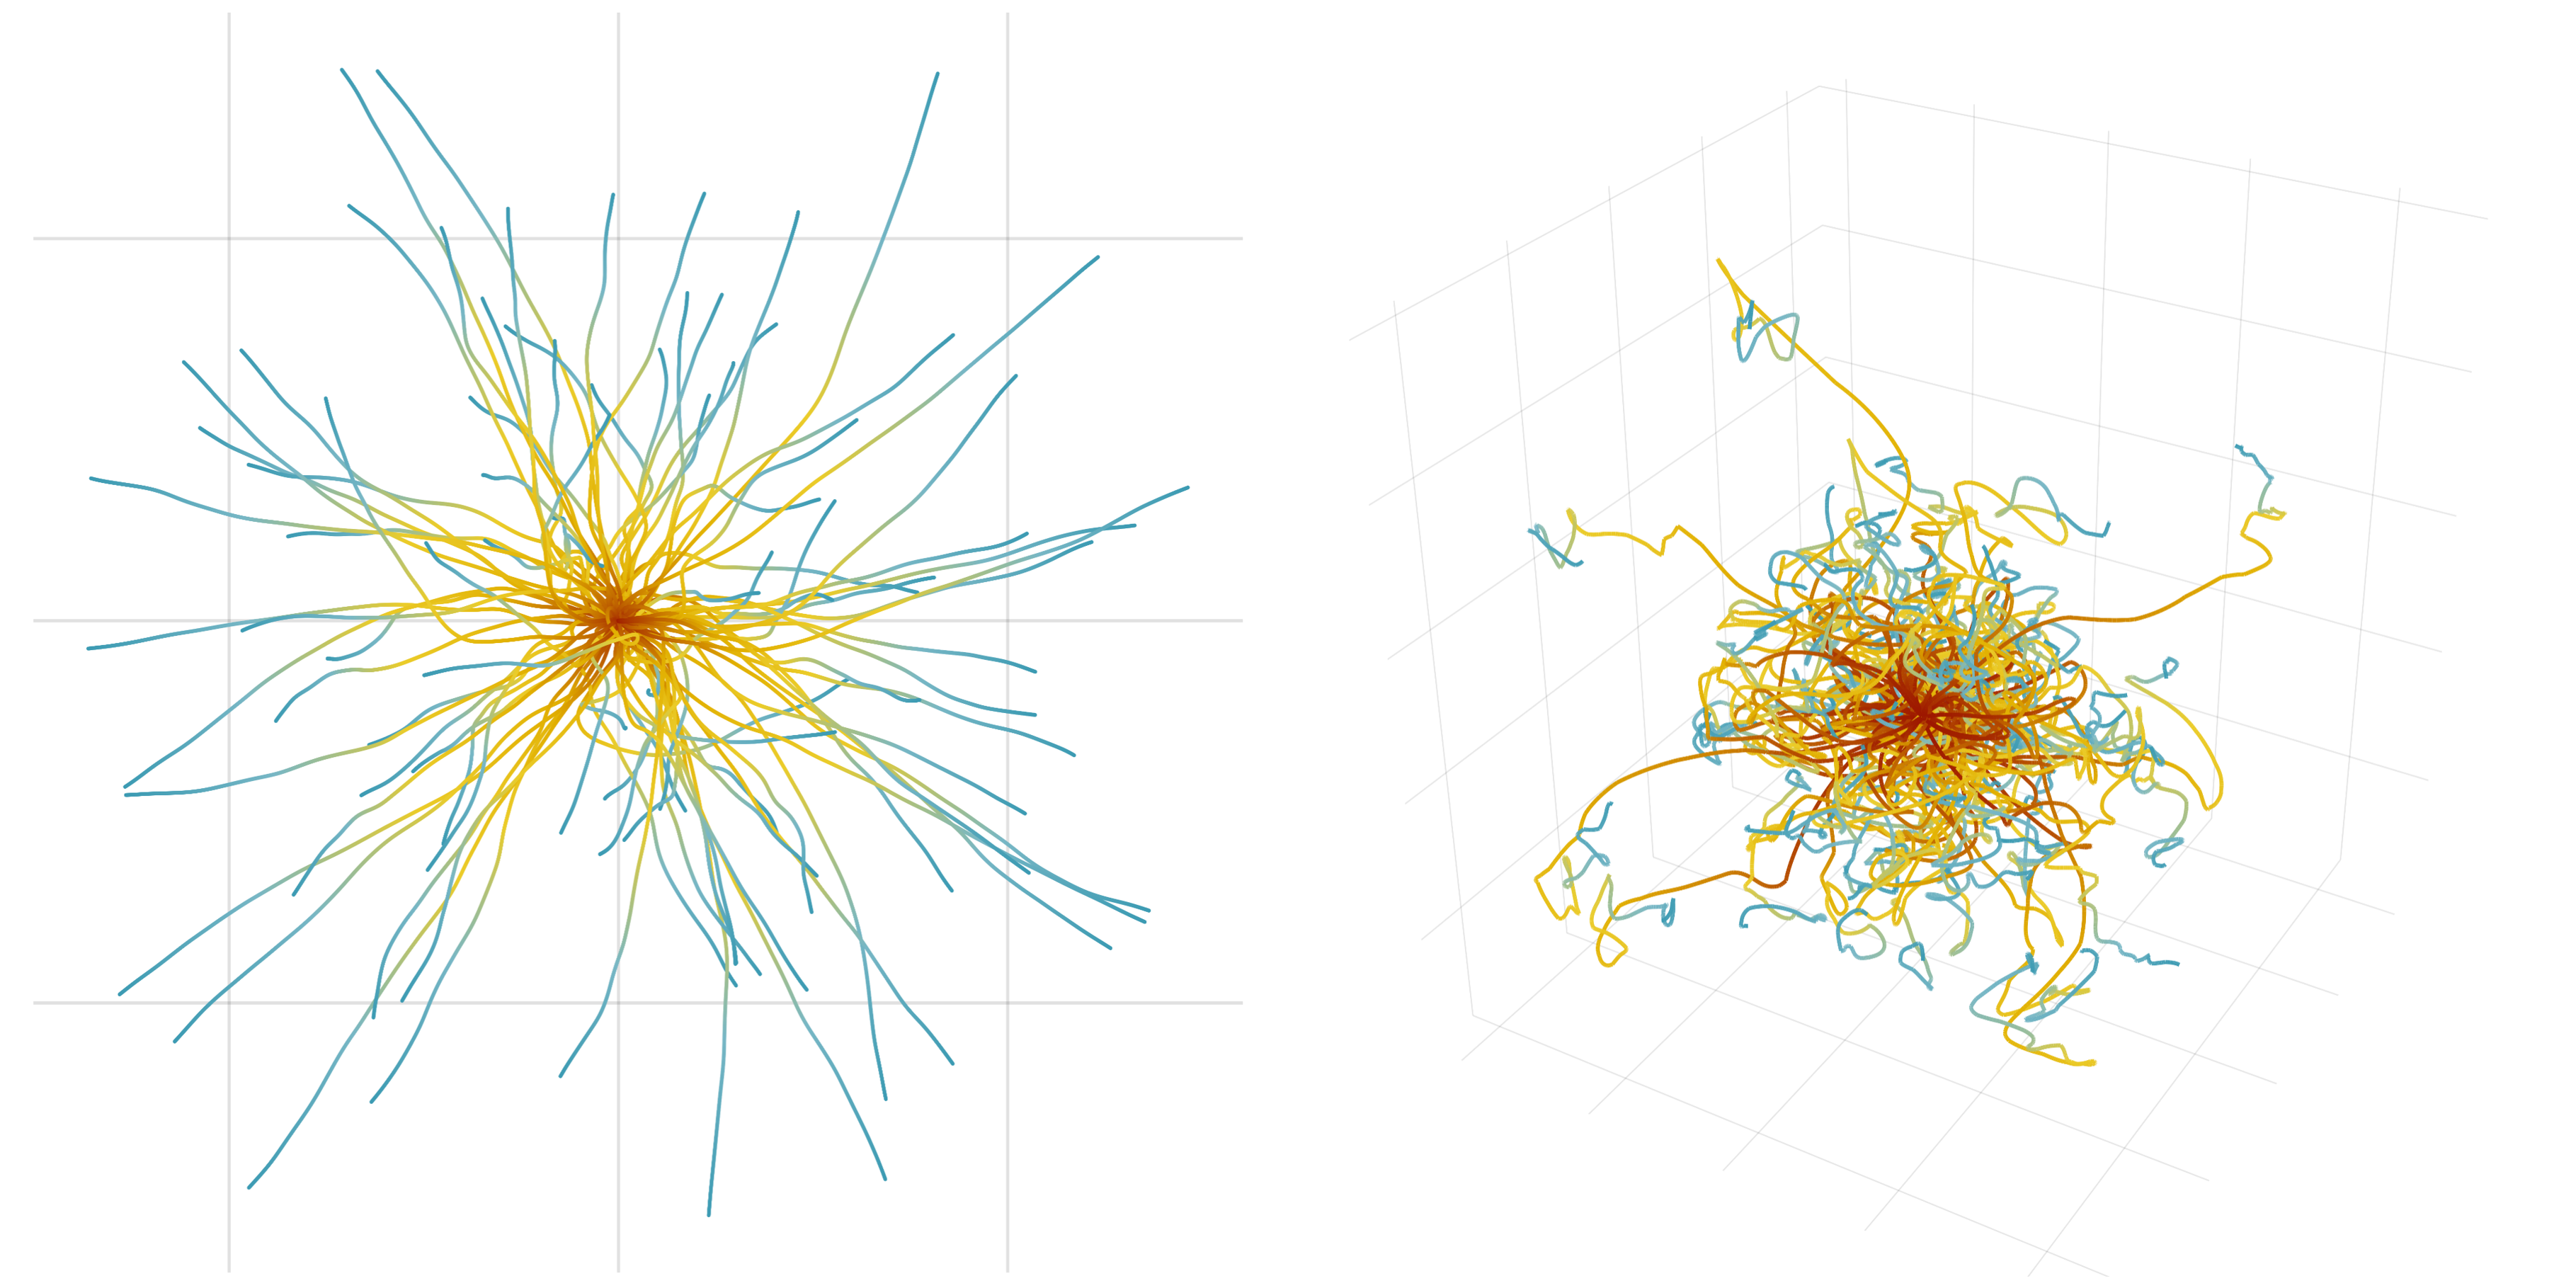
\includegraphics[height=0.7\paperheight]{images/trajectories_cpic.png}} 
    \\[10pt]  
   };
}
\begin{frame}{Outline}
    \begin{center}
        \tableofcontents
    \end{center}
\end{frame}
\setbeamertemplate{background}{}

\setcounter{framenumber}{0}
\setbeamertemplate{footline}[progress bar]
\setbeamercolor{progress bar}{fg=palteal,bg=palteal!40}
\addtobeamertemplate{headline}{}{\vspace{1cm}\hfill\circcounter\hspace*{1cm}}
\addtobeamertemplate{frametitle}{\vspace{-0.8cm}}{}

%%%%%%%%%%%%%%%%%%%%%%%%%%%%%%%%%%%%%%%%%
%%%%%%%%%%%%%%%% SECTION %%%%%%%%%%%%%%%%
%%%%%%%%%%%%%%%%%%%%%%%%%%%%%%%%%%%%%%%%%

\section{Heavy-ion collisions}

%%%%%%%%%%%%%%%%%%%%%%%%%%%%%%%%%%%%%%%%%
%%%%%%%%%%%%%% SUBSECTION %%%%%%%%%%%%%%%
%%%%%%%%%%%%%%%%%%%%%%%%%%%%%%%%%%%%%%%%%

\subsection{Initial stage}

%%%%%%%%%%%%%%%%%%%%%%%%%%%%%%%%%%%%%%%%%
%%%%%%%%%%%%%%%%% SLIDE %%%%%%%%%%%%%%%%%
%%%%%%%%%%%%%%%%%%%%%%%%%%%%%%%%%%%%%%%%%

\begin{frame}
    \frametitle{Heavy-ion collisions}
    \framesubtitle{Stages at weak coupling}
    \vspace{-15pt}
    \begin{columns}[onlytextwidth,t]
        \column{.02\textwidth}
        \column{.47\textwidth}
            \begin{center}
                \vspace{-5pt}
                \begin{tikzpicture}
                    \node[anchor=south west,inner sep=0] at (0,0) {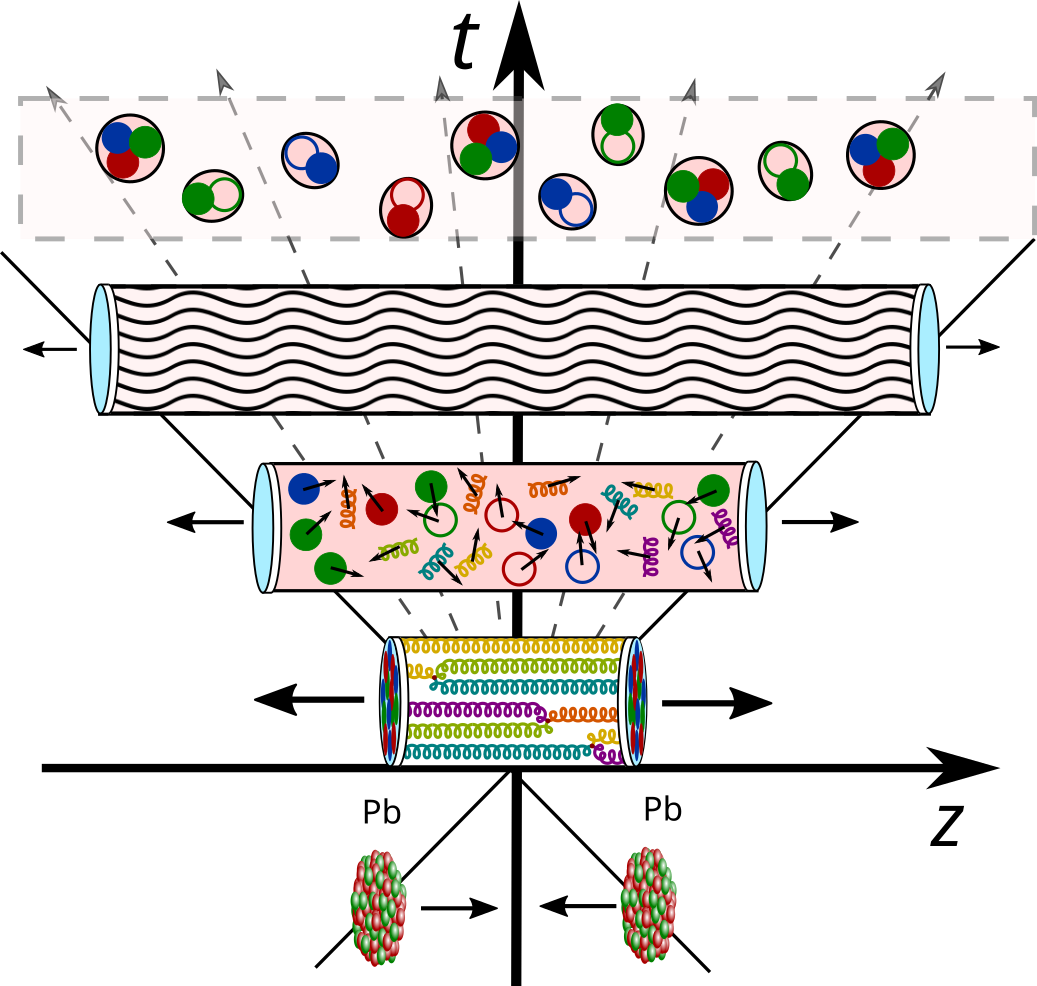
\includegraphics[width=0.95\textwidth]{images/cover_figure_A01.png}};
                \end{tikzpicture}
            \end{center}
        \column{.02\textwidth}
        \column{.47\textwidth}
            \vspace{10pt}
            \begin{center}
            \begin{custombox2}{\color{normal}Collision stages}{lightgray}
                \small
                \begin{varwidth}{0.8\textwidth}
                \begin{itemize}\itemsep0em 
                    \setbeamertemplate{itemize item}{\raisebox{0.2em}{\scalebox{0.7}{${\color{normal}\blacktriangleright}$}}} 
                    \item {Before collision {\scriptsize $\tau\leq 0\,\mathrm{fm/c}$}}\\[1pt]
                        {\color{lightgray}\scriptsize Gluon field of high-energy nucleus}
                    \setbeamertemplate{itemize item}{\raisebox{0.2em}{\scalebox{0.7}{${\color{palviolet}\blacktriangleright}$}}} \item {{\bfseries\color{palviolet} Initial stage} {\scriptsize $\tau\lesssim
                    0.3\,\mathrm{fm/c}$}}\\[1pt]
                        {\color{lightgray}\scriptsize {\bfseries\color{palviolet}Glasma} strong classical gluon fields}
                    \setbeamertemplate{itemize item}{\raisebox{0.2em}{\scalebox{0.7}{${\color{normal}\blacktriangleright}$}}} \item Thermalization {\scriptsize$\tau\lesssim
                    1\,\mathrm{fm/c}$}\\[1pt] 
                        {\color{lightgray}\scriptsize Effective kinetic theory} 
                        % \\ {\color{lightgray}\scriptsize Quasiparticle distribution function}
                    \item Equilibration {\scriptsize $\tau\lesssim 10\,\mathrm{fm/c}$}\\[1pt]
                    {\color{lightgray}\scriptsize Relativistic hydrodynamics} 
                    % \\ {\color{lightgray}\scriptsize Energy-momentum tensor}
                    \item Final stages {\scriptsize $\tau\geq 10\,\mathrm{fm/c}$}\\[1pt]
                    {\color{lightgray}\scriptsize Particlization, hadronization}
                \end{itemize}
                \end{varwidth}
            \end{custombox2}
            \end{center}
        \column{.02\textwidth}
    \end{columns}
    \blfootnote{\scriptsize Berges, Heller, Mazeliauskas, Venugopalan \href{https://arxiv.org/abs/2005.12299}{{\color{palgold}\texttt{[2005.12299]$^\text{\tiny\faExternalLink}$}}}, Schlichting, Teaney \href{https://arxiv.org/abs/1908.02113}{{\color{palgold}\texttt{[1908.02113]$^\text{\tiny\faExternalLink}$}}}}
\end{frame}

%%%%%%%%%%%%%%%%%%%%%%%%%%%%%%%%%%%%%%%%%
%%%%%%%%%%%%%%%%% SLIDE %%%%%%%%%%%%%%%%%
%%%%%%%%%%%%%%%%%%%%%%%%%%%%%%%%%%%%%%%%%

\begin{frame}[noframenumbering]
    \frametitle{Initial stage of collision}
    % \framesubtitle{Stages at weak coupling}
    \vspace{-10pt}
    \begin{columns}[onlytextwidth,t]
        \column{.02\textwidth}
        \column{.47\textwidth}
            \begin{center}
                \vspace{-5pt}
                \begin{tikzpicture}
                    \node[anchor=south west,inner sep=0] at (0,0) {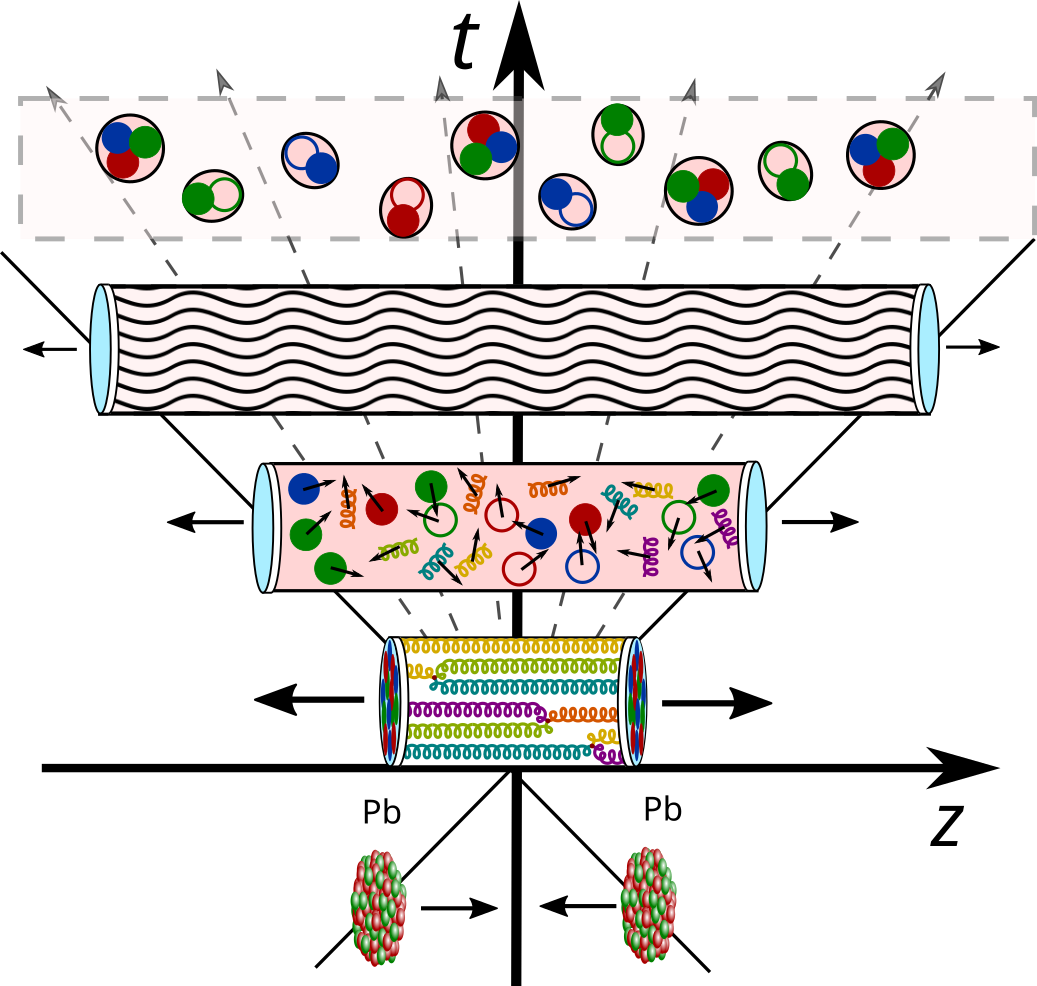
\includegraphics[width=0.95\textwidth]{images/cover_figure_A01.png}};
                    \draw<1>[white, fill=white, fill opacity=0.9] (0.0,2.45) rectangle (6.8,6.5);
                    \draw<1>[palviolet,thick,fill=palviolet,fill opacity=0.1,rounded corners=3pt] (0.1,-0.1) rectangle (6.7,2.45);
                \end{tikzpicture}
            \end{center}
        \column{.02\textwidth}
        \column{.47\textwidth}
            \vspace{20pt}
            \begin{center}
            \begin{custombox2}{Glasma initial stage}{palviolet}
                \small
                \begin{varwidth}{0.76\textwidth}
                \begin{itemize}\itemsep0em 
                    \setbeamertemplate{itemize item}{\raisebox{0.2em}{\scalebox{0.7}{${\color{palviolet}\blacktriangleright}$}}} 
                    \item {Color glass condensate}\\[1pt]
                        {\color{lightgray}\scriptsize QCD in the high-energy limit}
                    \item Weakly coupled $\alpha_s\ll 1$
                    \item {\bfseries Classical gluon fields}\\[1pt]
                        {\color{lightgray}\scriptsize Occupation number $\sim 1/\alpha_s\gg 1$}
                    \item Non-perturbative 
                    \item {\bfseries Lattice gauge theory}\\[1pt]
                        {\color{lightgray}\scriptsize Numerical solution}
                    \item {\bfseries Out-of-equilibrium}
                    
                \end{itemize}
                \end{varwidth}
            \end{custombox2}
            \end{center}
        \column{.02\textwidth}
    \end{columns}
    \blfootnote{\scriptsize Lappi \href{https://arxiv.org/abs/hep-ph/0606207}{{\color{palviolet}\texttt{[hep-ph/0606207]}$^\text{\tiny\faExternalLink}$}}, Gelis \href{https://arxiv.org/abs/1211.3327}{{\color{palviolet}\texttt{[1211.3327]}$^\text{\tiny\faExternalLink}$}}}
\end{frame}


%%%%%%%%%%%%%%%%%%%%%%%%%%%%%%%%%%%%%%%%%
%%%%%%%%%%%%%% SUBSECTION %%%%%%%%%%%%%%%
%%%%%%%%%%%%%%%%%%%%%%%%%%%%%%%%%%%%%%%%%

\subsection{Heavy quarks as probes}

%%%%%%%%%%%%%%%%%%%%%%%%%%%%%%%%%%%%%%%%%
%%%%%%%%%%%%%%%%% SLIDE %%%%%%%%%%%%%%%%%
%%%%%%%%%%%%%%%%%%%%%%%%%%%%%%%%%%%%%%%%%

\begin{frame}
    \frametitle{Heavy quarks as probes}
    \framesubtitle{Approaches and kinematic regimes}

    \begin{columns}[onlytextwidth,t]
        \column{.02\textwidth}
        \column{.57\textwidth}
            \vspace{-20pt}
            \begin{center}
                \begin{tikzpicture}
                    \node[anchor=south west,inner sep=0] at (0,0) {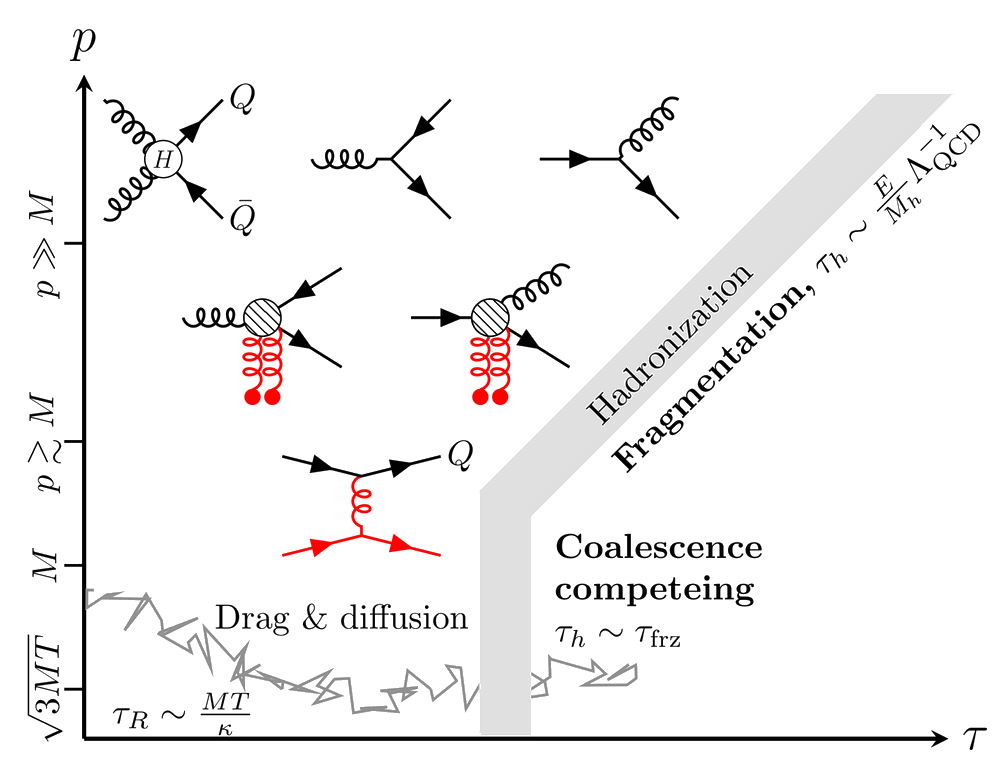
\includegraphics[width=0.95\textwidth]{images/HP24-Weiyao-Ke-HF-Theory-2-crop-white.png}};
                \end{tikzpicture}
            \end{center}
        \column{.02\textwidth}
        \column{.37\textwidth}
        \vspace{10pt}
        \begin{center}
            \begin{custombox2}{\color{normal}Approaches}{lightgray}
                \small
                \begin{varwidth}{0.85\textwidth}
                \begin{itemize}\itemsep0em 
                    \setbeamertemplate{itemize item}{\raisebox{0.2em}{\scalebox{0.7}{${\color{normal}\blacktriangleright}$}}} 
                    \item pQCD production\\[1pt]
                        {\color{lightgray}\scriptsize FONLL and GM-VFNS at NLO+NLL accuracy}
                    \item Transport models\\[1pt]
                        {\color{lightgray}\scriptsize Boltzmann, Langevin, Fokker-Planck equations}
                    \item Hadronization\\[1pt]
                        {\color{lightgray}\scriptsize Fragmentation + coalescence}  
                \end{itemize}
                \end{varwidth}
            \end{custombox2}
            \end{center}
        \column{.02\textwidth}
    \end{columns}

    \vspace{-5pt}    
    \blfootnote{\scriptsize Ke - \textit{Open Heavy Flavor: Theory} \href{https://indico.cern.ch/event/1339555/contributions/6038190/}{{\color{red}\texttt{[Hard Probes 24]$^\text{\tiny\faExternalLink}$}}}}
\end{frame}

%%%%%%%%%%%%%%%%%%%%%%%%%%%%%%%%%%%%%%%%%
%%%%%%%%%%%%%%%%% SLIDE %%%%%%%%%%%%%%%%%
%%%%%%%%%%%%%%%%%%%%%%%%%%%%%%%%%%%%%%%%%

\begin{frame}[noframenumbering]
    \frametitle{Heavy quarks as probes of the {\color{red}early stage}}
    % \framesubtitle{Recent focus on the early stage}

    \begin{center}
        \begin{tikzpicture}
            \node[anchor=south west,inner sep=0] at (0,0) {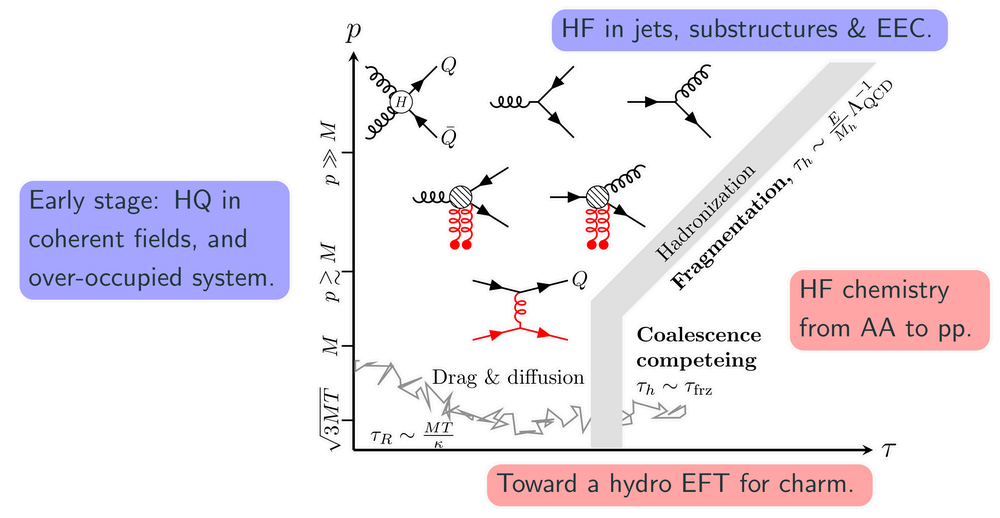
\includegraphics[width=0.8\textwidth]{images/HP24-Weiyao-Ke-HF-Theory-28-crop-white.png}};
            % \draw<1>[palgold,thick,fill=palgold,fill opacity=0.1,rounded corners=3pt] (0.0,4) rectangle (\textheight-0.5cm,4.0) node[opacity=1.0, pos=0, anchor=center, xshift=0.0\linewidth,text width=2cm,align=center]{{\Large\color{palgold}\bfseries This talk}};
            \draw<1>[white, fill=white, fill opacity=0.9] (4.3,0.85) rectangle (5.4,5.5);
            \draw<1>[red,thick,fill=red,fill opacity=0.1,rounded corners=3pt] (4.3,0.85) rectangle (5.4,5.5) node[opacity=1.0, pos=0.5, rotate=90, anchor=center, xshift=0.0 ,text width=6.2cm,align=center] {{\Large\color{red} Early stage}};
        \end{tikzpicture}
    \end{center}
    \vspace{-10pt}    
    \blfootnote{\scriptsize Ke - \textit{Open Heavy Flavor: Theory} \href{https://indico.cern.ch/event/1339555/contributions/6038190/}{{\color{red}\texttt{[Hard Probes 24]$^\text{\tiny\faExternalLink}$}}}}
\end{frame}

%%%%%%%%%%%%%%%%%%%%%%%%%%%%%%%%%%%%%%%%
%%%%%%%%%%%%%%% SECTION %%%%%%%%%%%%%%%%
%%%%%%%%%%%%%%%%%%%%%%%%%%%%%%%%%%%%%%%%

\section{Glasma}

%%%%%%%%%%%%%%%%%%%%%%%%%%%%%%%%%%%%%%%%%
%%%%%%%%%%%%%%%%% SLIDE %%%%%%%%%%%%%%%%%
%%%%%%%%%%%%%%%%%%%%%%%%%%%%%%%%%%%%%%%%%

\setbeamertemplate{background}{
\tikz[overlay,remember picture] \node[opacity=0.1, at=(current page.center), align=center] {\\[10pt]
{\transparent{0.2}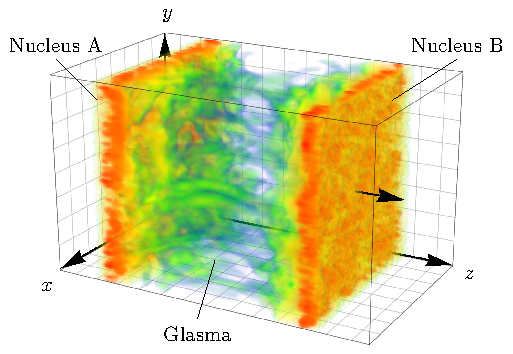
\includegraphics[height=0.8\paperheight]{images/fig1_overview.pdf}}};
}
\begin{frame}[plain,noframenumbering]{}
    \begin{center}
        \vspace{1cm}
        {\large\color{normal}Initial stage of pre-equilibrium}\\[0.3cm]
        {\huge\color{destacado}The glasma}
    \end{center}
\end{frame}
\setbeamertemplate{background}{}

%%%%%%%%%%%%%%%%%%%%%%%%%%%%%%%%%%%%%%%%%
%%%%%%%%%%%%%%%%% SLIDE %%%%%%%%%%%%%%%%%
%%%%%%%%%%%%%%%%%%%%%%%%%%%%%%%%%%%%%%%%%

\setbeamertemplate{background}{
\tikz[overlay,remember picture] \node[at=(current page.center), align=center] {\\[10pt]
{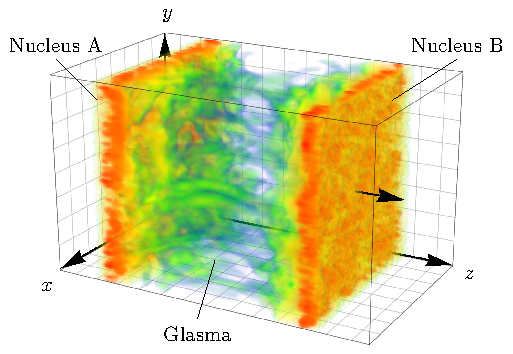
\includegraphics[height=0.7\paperheight]{images/fig1_overview.pdf}}};
}
\begin{frame}[plain,noframenumbering]
    \frametitle{\\ Glasma color fields}
    \blfootnote{\scriptsize Ipp, Müller  \href{https://arxiv.org/abs/1703.00017}{{\color{palgold}\texttt{[1703.00017]}$^\text{\tiny\faExternalLink}$}}}
\end{frame}
\setbeamertemplate{background}{}

%%%%%%%%%%%%%%%%%%%%%%%%%%%%%%%%%%%%%%%%
%%%%%%%%%%%%% SUBSECTION %%%%%%%%%%%%%%%
%%%%%%%%%%%%%%%%%%%%%%%%%%%%%%%%%%%%%%%%

% \subsection{Color glass condensate}

%%%%%%%%%%%%%%%%%%%%%%%%%%%%%%%%%%%%%%%%%
%%%%%%%%%%%%%%%%% SLIDE %%%%%%%%%%%%%%%%%
%%%%%%%%%%%%%%%%%%%%%%%%%%%%%%%%%%%%%%%%%

\setbeamertemplate{itemize item}{\raisebox{0.2em}{\scalebox{0.7}{${\color{normal}\blacktriangleright}$}}} 

\begin{frame}
    \frametitle{CGC and glasma}
    % \framesubtitle{QCD at high energy and small-$x$ physics}
    \vspace{-10pt}
    \begin{columns}[onlytextwidth,t]
       \column{.033\textwidth}
       \column{.35\textwidth}

            \begin{center}
                \footnotesize\color{lightgray}A high-energy nucleus contains \\ large numbers of {\bfseries\color{palviolet}soft gluons}
            \end{center}
            % \begin{itemize}\itemsep0em 
            %     \footnotesize\color{lightgray}
            %     \setbeamertemplate{itemize item}{\raisebox{0.2em}{\scalebox{0.6}{${\color{lightgray}\blacktriangleright}$}}}
            %     \item A high-energy nucleus contains mostly {\bfseries\color{palviolet}soft gluons}
            % \end{itemize}

            \vspace{5pt}
            \hspace{10pt}
            \begin{tikzpicture}[]
                \node[anchor=south west,inner sep=0] at (0,0) {\includegraphics[width=0.9\textwidth]{images/CFNS_talk_Salazar-3_crop_edit_final_v2.png}};
                \draw<1>[palviolet,line width=1pt,fill=palviolet,fill opacity=0.1,rounded corners=3pt] (2.2, 0) rectangle (4.8, 4.9);
            \end{tikzpicture}
        \column{.06\textwidth}
        \column{.55\textwidth}

            \vspace{-5pt}
           
            \begin{custombox2}{Color glass condensate}{lightgray}
                \small
                \begin{varwidth}{0.97\textwidth}
                \begin{itemize}\itemsep0em 
                    \setbeamertemplate{itemize item}{\raisebox{0.2em}{\scalebox{0.7}{${\color{lightgray}\blacktriangleright}$}}} 
                    \item 
                    Soft partons $\leftrightarrow$ {\color{palviolet}\bfseries gauge fields $\boldsymbol{A^\mu}$} generated by the hard partons $\leftrightarrow$ {\color{palteal}\bfseries color current $\boldsymbol{J^\mu}$}
                \end{itemize}
                \end{varwidth}
            \end{custombox2}

            % \begin{itemize}\itemsep0em 
            %     \footnotesize\color{lightgray}
            %     \setbeamertemplate{itemize item}{\raisebox{0.2em}{\scalebox{0.6}{${\color{lightgray}\blacktriangleright}$}}}
            %     \item Classical {\color{palviolet}gluon fields} $\rightarrow$ produced\\ by color {\color{pallightblue}nucleus current}
            % \end{itemize}
            \begin{itemize}\itemsep0em 
                \item Classical Yang-Mills equations
            \end{itemize}
            \vspace{20pt}
            \renewcommand{\eqnhighlightheight}{\vphantom{\mathcal{D}_\mu}\mathstrut}\begin{equation*}
                \hspace{-40pt}\eqnmark[normal]{dmu}{\mathscr{D}_\mu}\hspace{-3pt}\eqnmark[normal]{fmunu}{F^{\mu\nu}}\hspace{-3pt}={\color{palteal}\boldsymbol{J^\nu}}
                % {\color{lightgray}\rightarrow\,\text{input from CGC}} 
                \end{equation*}
                \annotate[yshift=+0.5em]{above, left}{dmu}{\scriptsize $\partial_\mu-\mathrm{i}g{\color{palviolet}\boldsymbol{A_\mu}}$}
                \annotate[yshift=-0.1em]{below}{fmunu}{\scriptsize $\partial_\mu{\color{palviolet}\boldsymbol{A_\nu}}-\partial_\nu{\color{palviolet}\boldsymbol{A_\mu}}-\mathrm{i}g[{\color{palviolet}\boldsymbol{A_\mu}},{\color{palviolet}\boldsymbol{A_\nu}}]$}
            \vspace{5pt}
            {\footnotesize
            \begin{itemize}\itemsep0em 
                % \setbeamertemplate{itemize item}{\raisebox{0.2em}{\scalebox{0.6}{${\color{lightgray}\blacktriangleright}$}}} 
                \item \textit{Before collision:} CGC fields\\[1pt] 
                {\color{lightgray} Analytical gluon field of a single nucleus}
                \item \textit{After collision:} {\color{palgold}\bfseries glasma fields}\\[1pt] 
                {\color{lightgray} Numerical gluon field of two colliding nuclei}
            \end{itemize}}
        \column{.033\textwidth}
    \end{columns}
    \blfootnote{\scriptsize Gelis, Iancu, Jalilian-Marian, Venugopalan \href{https://arxiv.org/abs/1002.0333}{{\color{palviolet}\texttt{[1002.0333]}$^\text{\tiny\faExternalLink}$}}, Lappi \href{https://arxiv.org/abs/hep-ph/0602189}{{\color{palgold}\texttt{[hep-ph/0602189]}$^\text{\tiny\faExternalLink}$}}}
\end{frame}


%%%%%%%%%%%%%%%%%%%%%%%%%%%%%%%%%%%%%%%%%
%%%%%%%%%%%%%% SUBSECTION %%%%%%%%%%%%%%%
%%%%%%%%%%%%%%%%%%%%%%%%%%%%%%%%%%%%%%%%%

\subsection{Features of the glasma}

%%%%%%%%%%%%%%%%%%%%%%%%%%%%%%%%%%%%%%%%%
%%%%%%%%%%%%%%%%% SLIDE %%%%%%%%%%%%%%%%%
%%%%%%%%%%%%%%%%%%%%%%%%%%%%%%%%%%%%%%%%%

\begin{frame}
    \frametitle{Features of the glasma}
    % \framesubtitle{Flux tubes, strong fields, correlation domains}
    \vspace{-10pt}
    \begin{columns}[onlytextwidth,t]
        \column{.05\textwidth}
        \column{.3\textwidth}

        \begin{custombox2}{{\normalsize Flux tubes}}{palteal}
            \begin{varwidth}{0.99\columnwidth}
            \begin{itemize}\itemsep0em 
                \setbeamertemplate{itemize item}{\raisebox{0.2em}{\scalebox{0.7}{${\color{palteal}\blacktriangleright}$}}} 
                \scriptsize
                \item Initially only longitudinal electric and magnetic fields
            \end{itemize}
            \end{varwidth}
        \end{custombox2}

       \column{.025\textwidth}
       \column{.3\textwidth}
       \begin{custombox2}{{\normalsize Strong fields}}{palviolet}
            \begin{varwidth}{0.95\columnwidth}
            \begin{itemize}\itemsep0em 
                \setbeamertemplate{itemize item}{\raisebox{0.2em}{\scalebox{0.7}{${\color{palviolet}\blacktriangleright}$}}} 
                \scriptsize
                \item Strong longitudinal fields, dilute after $\tau\sim 1/{\boldsymbol{Q_s}}$
            \end{itemize}
            \end{varwidth}
        \end{custombox2}

        \column{.025\textwidth}
        \column{.3\textwidth}
        \begin{custombox2}{{\normalsize Correlation domains}}{palgold}
            \begin{varwidth}{0.99\columnwidth}
            \begin{itemize}\itemsep0em 
                \setbeamertemplate{itemize item}{\raisebox{0.2em}{\scalebox{0.7}{${\color{palgold}\blacktriangleright}$}}} 
                \scriptsize
                \item Fields correlated inside flux tubes of size $\sim 1/{\boldsymbol{Q_s}}$ 
            \end{itemize}
            \end{varwidth}
        \end{custombox2}
 
        % \column{.025\textwidth}
    \end{columns}

    \begin{columns}[onlytextwidth,t]
        \column{.03\textwidth}
        \column{.3\textwidth}

        \vspace{5pt}
        \begin{center}
            \begin{figure}
                \centering
                \hspace{-5pt}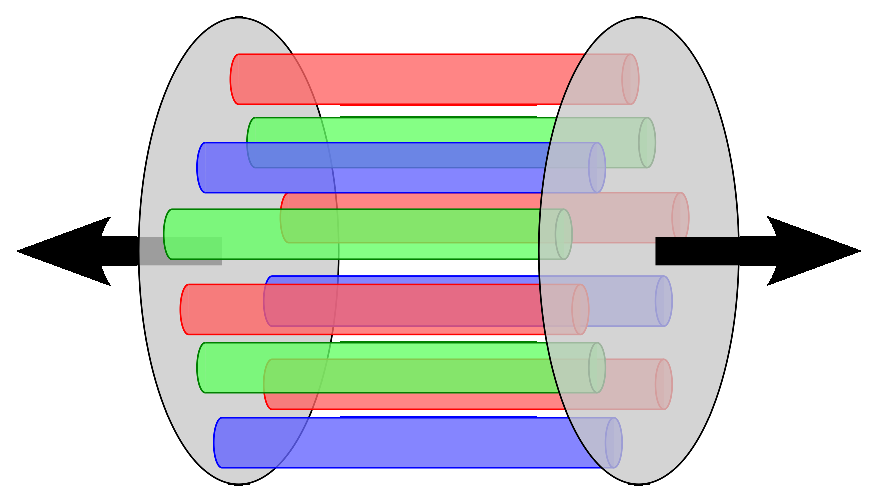
\includegraphics[width=0.9\textwidth]{images/glasma.eps}
            \end{figure}
        \end{center}

       \column{.025\textwidth}
       \column{.3\textwidth}
        % \begin{center}
        %     \begin{figure}
        %         \centering
        %         \hspace{-5pt}\includegraphics[width=0.9\textwidth]{images/components.eps}
        %     \end{figure}
        % \end{center}
        \begin{center}
            \begin{tikzpicture}
                \node[anchor=south west,inner sep=0] at (0,0) {\includegraphics[width=0.9\textwidth]{images/components.eps}};
                % \draw<1>[white, fill=white, fill opacity=0.9] (4.3,0.85) rectangle (5.4,5.5);
                % \draw<1>[red,thick,fill=red,fill opacity=0.1,rounded corners=3pt] (0.1,0.85) rectangle (1.0, 2.0);
            \end{tikzpicture}
        \end{center}

        \column{.025\textwidth}
        \column{.3\textwidth}
        \begin{center}
            \begin{figure}
                \centering
                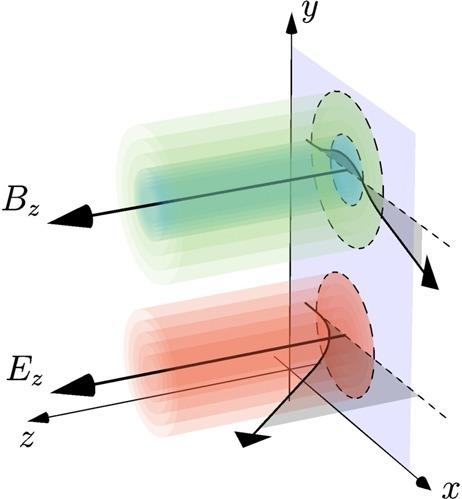
\includegraphics[width=0.7\textwidth]{images/1-s2.0-S0370269320306134-gr003_lrg.jpg}
            \end{figure}
        \end{center}

        \column{.05\textwidth}
    \end{columns}

    \vspace{5pt}
    \begin{itemize}\itemsep0em 
        \setbeamertemplate{itemize item}{\raisebox{0.2em}{\scalebox{0.5}{${\color{normal}\blacktriangleright}$}}}
        \item \begin{center}\footnotesize Glasma physical parameter: gluon {\bfseries saturation momentum $\boldsymbol{Q_s}$}\end{center}
        % \setbeamertemplate{itemize item}{\raisebox{0.2em}{\scalebox{0.6}{${\color{lightgray}\blacktriangleright}$}}}
        \item \begin{center}\footnotesize Heavy quarks probe these properties of the glasma fields\,\end{center}
    \end{itemize}

    \vspace{-5pt}
    \blfootnote{\scriptsize Fukushima \href{https://arxiv.org/abs/1603.02340}{{\color{palteal}\texttt{[1603.02340]}$^\text{\tiny\faExternalLink}$}}, Lappi \href{https://arxiv.org/abs/hep-ph/0606207}{{\color{palviolet}\texttt{[hep-ph/0606207]}$^\text{\tiny\faExternalLink}$}}, Ipp, Müller, Schuh \href{https://arxiv.org/abs/2009.14206}{{\color{palgold}\texttt{[2009.14206]}$^\text{\tiny\faExternalLink}$}}
    }
\end{frame}


%%%%%%%%%%%%%%%%%%%%%%%%%%%%%%%%%%%%%%%%%
%%%%%%%%%%%%%%%% SECTION %%%%%%%%%%%%%%%%
%%%%%%%%%%%%%%%%%%%%%%%%%%%%%%%%%%%%%%%%%

\section{Heavy quarks in glasma}

%%%%%%%%%%%%%%%%%%%%%%%%%%%%%%%%%%%%%%%%%
%%%%%%%%%%%%%%%%% SLIDE %%%%%%%%%%%%%%%%%
%%%%%%%%%%%%%%%%%%%%%%%%%%%%%%%%%%%%%%%%%

\setbeamertemplate{background}{
\tikz[overlay,remember picture] \node[opacity=0.1, at=(current page.center), align=center] {\\[10pt]
{\transparent{0.1}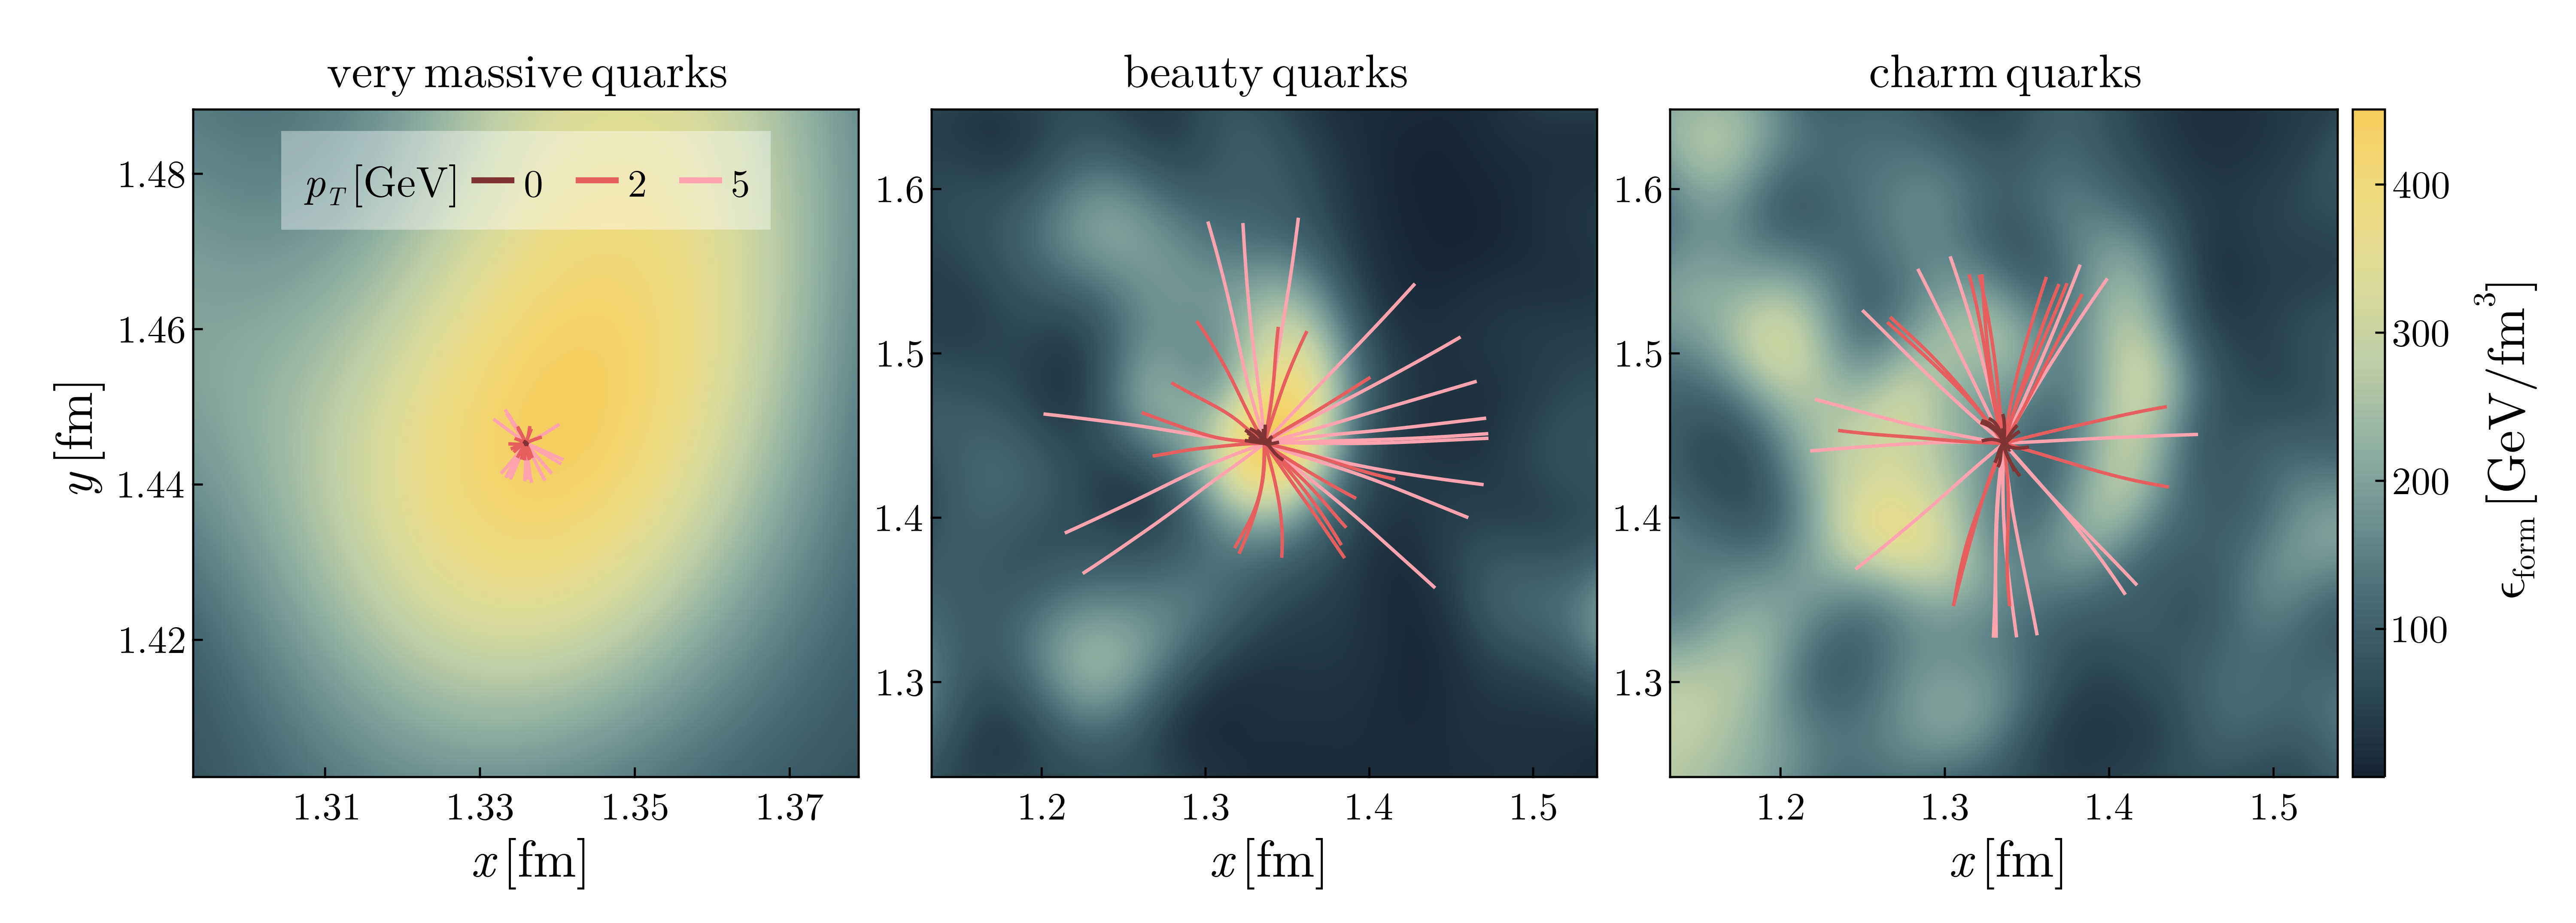
\includegraphics[height=0.6\paperheight]{images/hqs_flux_tubes_background+hqs.png}}};
}
\setbeamertemplate{itemize item}{\raisebox{0.2em}{\scalebox{0.7}{${\color{normal}\blacktriangleright}$}}} 
\begin{frame}[plain,noframenumbering]{}
    \begin{center}
        \vspace{1cm}
        {\large\color{normal}Probes of the initial stage of pre-equilibrium}\\[0.3cm]
        {\huge\color{destacado}Heavy quarks in glasma}\\[0.3cm]
    \end{center}
\end{frame}
\setbeamertemplate{background}{}

%%%%%%%%%%%%%%%%%%%%%%%%%%%%%%%%%%%%%%%%%
%%%%%%%%%%%%%%%%% SLIDE %%%%%%%%%%%%%%%%%
%%%%%%%%%%%%%%%%%%%%%%%%%%%%%%%%%%%%%%%%%

\setbeamertemplate{background}{
\tikz[overlay,remember picture] \node[at=(current page.center), align=center] {\\[20pt]
{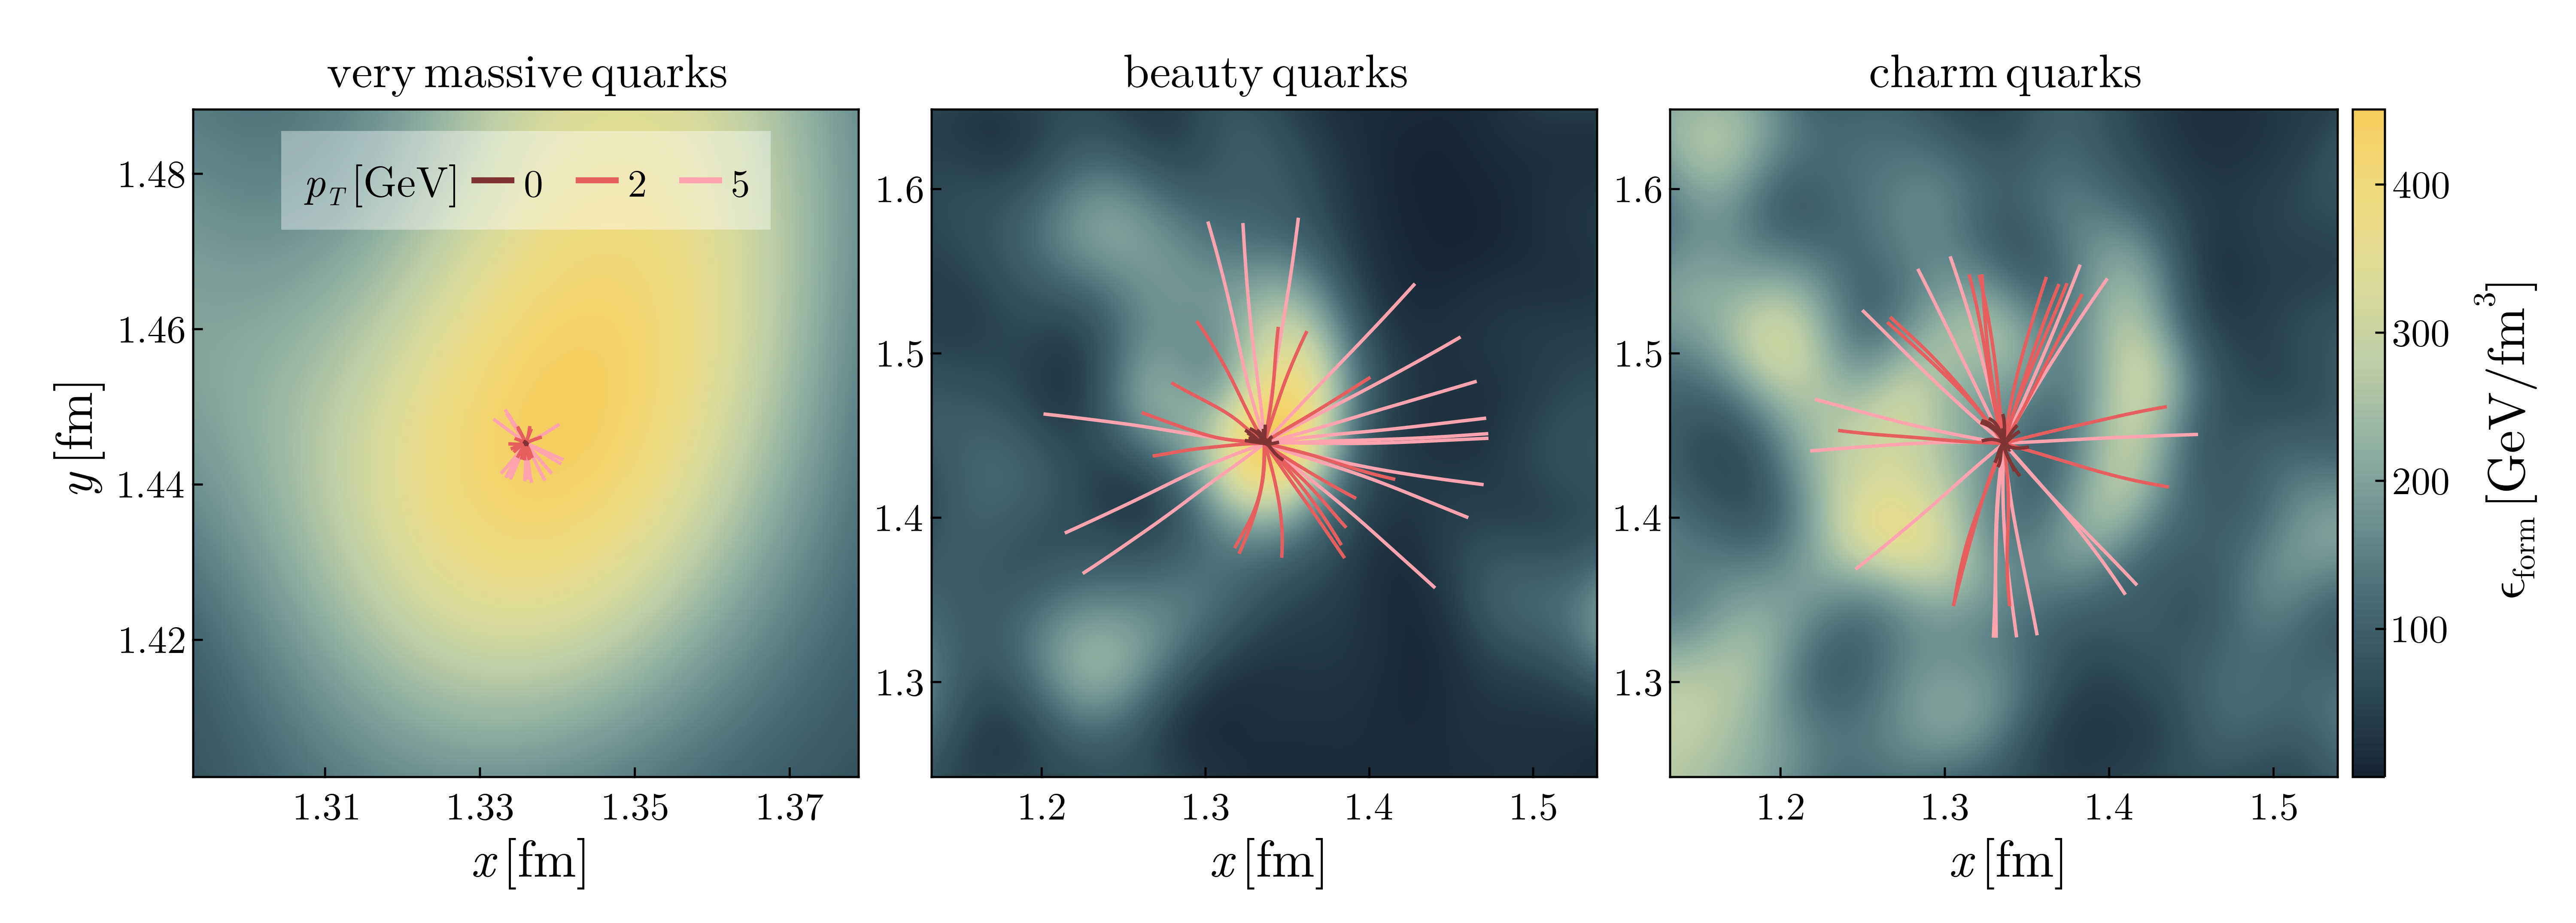
\includegraphics[height=0.6\paperheight]{images/hqs_flux_tubes_background+hqs.png}}};
}
\setbeamertemplate{itemize item}{\raisebox{0.2em}{\scalebox{0.7}{${\color{normal}\blacktriangleright}$}}} 
\begin{frame}[plain,noframenumbering]{}
    \frametitle{\\ Heavy quarks in glasma}
    \framesubtitle{Probing the glasma correlation domains}
    \blfootnote{\scriptsize Avramescu, Băran, Greco, Ipp, Müller, Ruggieri  \href{https://arxiv.org/abs/2303.05599}{{\color{palgold}\texttt{[2303.05599]}$^\text{\tiny\faExternalLink}$}}}
\end{frame}
\setbeamertemplate{background}{}

%%%%%%%%%%%%%%%%%%%%%%%%%%%%%%%%%%%%%%%%%
%%%%%%%%%%%%%% SUBSECTION %%%%%%%%%%%%%%%
%%%%%%%%%%%%%%%%%%%%%%%%%%%%%%%%%%%%%%%%%

\subsection{Transport equations}

% %%%%%%%%%%%%%%%%%%%%%%%%%%%%%%%%%%%%%%%%%
% %%%%%%%%%%%%%%%%% SLIDE %%%%%%%%%%%%%%%%%
% %%%%%%%%%%%%%%%%%%%%%%%%%%%%%%%%%%%%%%%%%

\begin{frame}
    \frametitle{Particles in Yang-Mills fields}
    \framesubtitle{Wong's equations of motion}
        \setbeamertemplate{itemize item}{\raisebox{0.2em}{\scalebox{0.7}{${\color{ming}\blacktriangleright}$}}} 
   \begin{center}
    \begin{custombox2}{Classical transport equations}{lightgray}
        \small
        \begin{varwidth}{0.72\textwidth}
        \begin{itemize}\itemsep0em 
            \setbeamertemplate{itemize item}{\raisebox{0.2em}{\scalebox{0.7}{${\color{lightgray}\blacktriangleright}$}}} 
            \item \begin{center}Wong's equations $\leftrightarrow$ classical equations of motion for particles\\
            $({\color{customblue}x^\mu},{\color{customred}p^\mu},{\color{customyellow}Q})$ evolving in a Yang-Mills background field ${\color{starrysecond}A^\mu}$\end{center} 
        \end{itemize}
        \end{varwidth}
    \end{custombox2}

    %    Wong's equations $\leftrightarrow$ classical equations of motion for particles $({\color{customblue}x^\mu},{\color{customred}p^\mu},{\color{customyellow}Q})$ \\
    % evolving in a Yang-Mills background field ${\color{starrysecond}A^\mu}$
   \end{center} 
        \vspace{1cm}
        \renewcommand{\eqnhighlightheight}{\vphantom{x}}
        \begin{equation*}
            \frac{\d}{\d\hspace{-0.1cm}\eqnmark[destacado]{tau}{\boldsymbol{\tau}}\hspace{-0.2cm}}\eqnmark[customblue]{xmu}{x^\mu}=\frac{{\color{customred}p^\mu}}{\eqnmark[destacado]{m}{m}},\qquad \eqnmark[destacado]{Ddtau}{\frac{\mathrm{D}}{\d\boldsymbol{\tau}}}\hspace{-0.2cm}\eqnmark[customred]{pmu}{p^\mu}=2\hspace{-0.1cm}\eqnmark[destacado]{g}{g}\hspace{-0.1cm}\tr{{\color{customyellow}Q}F^{\mu\nu}[\hspace{-0.1cm}\eqnmark[starrysecond]{amu}{A^\mu}\hspace{-0.1cm}]}\frac{{\color{customred}p_\nu}}{m},\qquad 
            \underbrace{\frac{\d}{\d\boldsymbol{\tau}}\hspace{-0.1cm}\eqnmark[customyellow]{Q}{Q}\hspace{-0.1cm}=-\mathrm{i}g [{\color{starrysecond}A_\mu},{\color{customyellow}Q}]\,\frac{{\color{customred}p^\mu}}{m}}_{\substack{\text{\footnotesize color rotation}\,\rightarrow\,{\color{customgreen}\mathcal{U}}\in\,\mathrm{SU(3)} \\[0.2cm] {\color{customyellow}Q}(\boldsymbol{\tau})=\,{\color{customgreen}\mathcal{U}}(\boldsymbol{\tau},\boldsymbol{\tau}^\prime){\color{customyellow}Q}(\boldsymbol{\tau^\prime})\,{\color{customgreen}\mathcal{U}^\dagger}(\boldsymbol{\tau},\boldsymbol{\tau}^\prime)}}
            \end{equation*}
            \annotate[yshift=1.2em]{above}{xmu}{coordinate}
            \annotate[yshift=1.2em]{above}{pmu}{momentum}
            \annotate[yshift=-0.5em]{below, right}{m}{\tiny mass}
            \annotate[yshift=-1.5em]{below, right}{Ddtau}{\tiny covariant derivative}
            \annotate[yshift=-1.5em]{below, right}{tau}{\tiny proper time}
            \annotate[yshift=-0.7em]{below, right}{g}{\tiny coupling constant}
            \annotate[yshift=1.2em]{above}{Q}{color charge}
            \annotate[yshift=1.2em]{above, right}{amu}{gauge field}

    \begin{itemize}\itemsep0em 
        \setbeamertemplate{itemize item}{\raisebox{0.2em}{\scalebox{0.7}{${\color{starrysecond}\blacktriangleright}$}}} 
        \item \begin{center}\footnotesize Solve the classical transport equations with {\color{starrysecond}$A^\mu$} the {\color{starrysecond}glasma field}\end{center} 
        \setbeamertemplate{itemize item}{\raisebox{0.2em}{\scalebox{0.7}{${\color{palgold}\blacktriangleright}$}}} 
        \item \begin{center}\footnotesize Simulation code \href{https://github.com/avramescudana/curraun/tree/wong}{\color{palgold}\texttt{github.com/avramescudana/curraun/tree/wong}$^\text{\tiny\faGithub}$}\end{center} 
    \end{itemize}
\end{frame}

%%%%%%%%%%%%%%%%%%%%%%%%%%%%%%%%%%%%%%%%%
%%%%%%%%%%%%%%%%% SLIDE %%%%%%%%%%%%%%%%%
%%%%%%%%%%%%%%%%%%%%%%%%%%%%%%%%%%%%%%%%%

\begin{frame}
    \frametitle{Particles in glasma fields}
    \framesubtitle{Visualizing the trajectories}
    \vspace{-0.5cm}
    \begin{columns}[onlytextwidth,t]
        \column{.025\textwidth}
       \column{.3\textwidth}
            \begin{itemize}\itemsep0em 
                \setbeamertemplate{itemize item}{\raisebox{0.2em}{\scalebox{0.7}{${\color{normal}\blacktriangleright}$}}} 
                \item \begin{center}\footnotesize Change in {\bfseries coordinates} due to momentum kicks\end{center}
            \end{itemize}
                \vspace{-20pt}
                \begin{figure}[!hbt]
                    \centering
                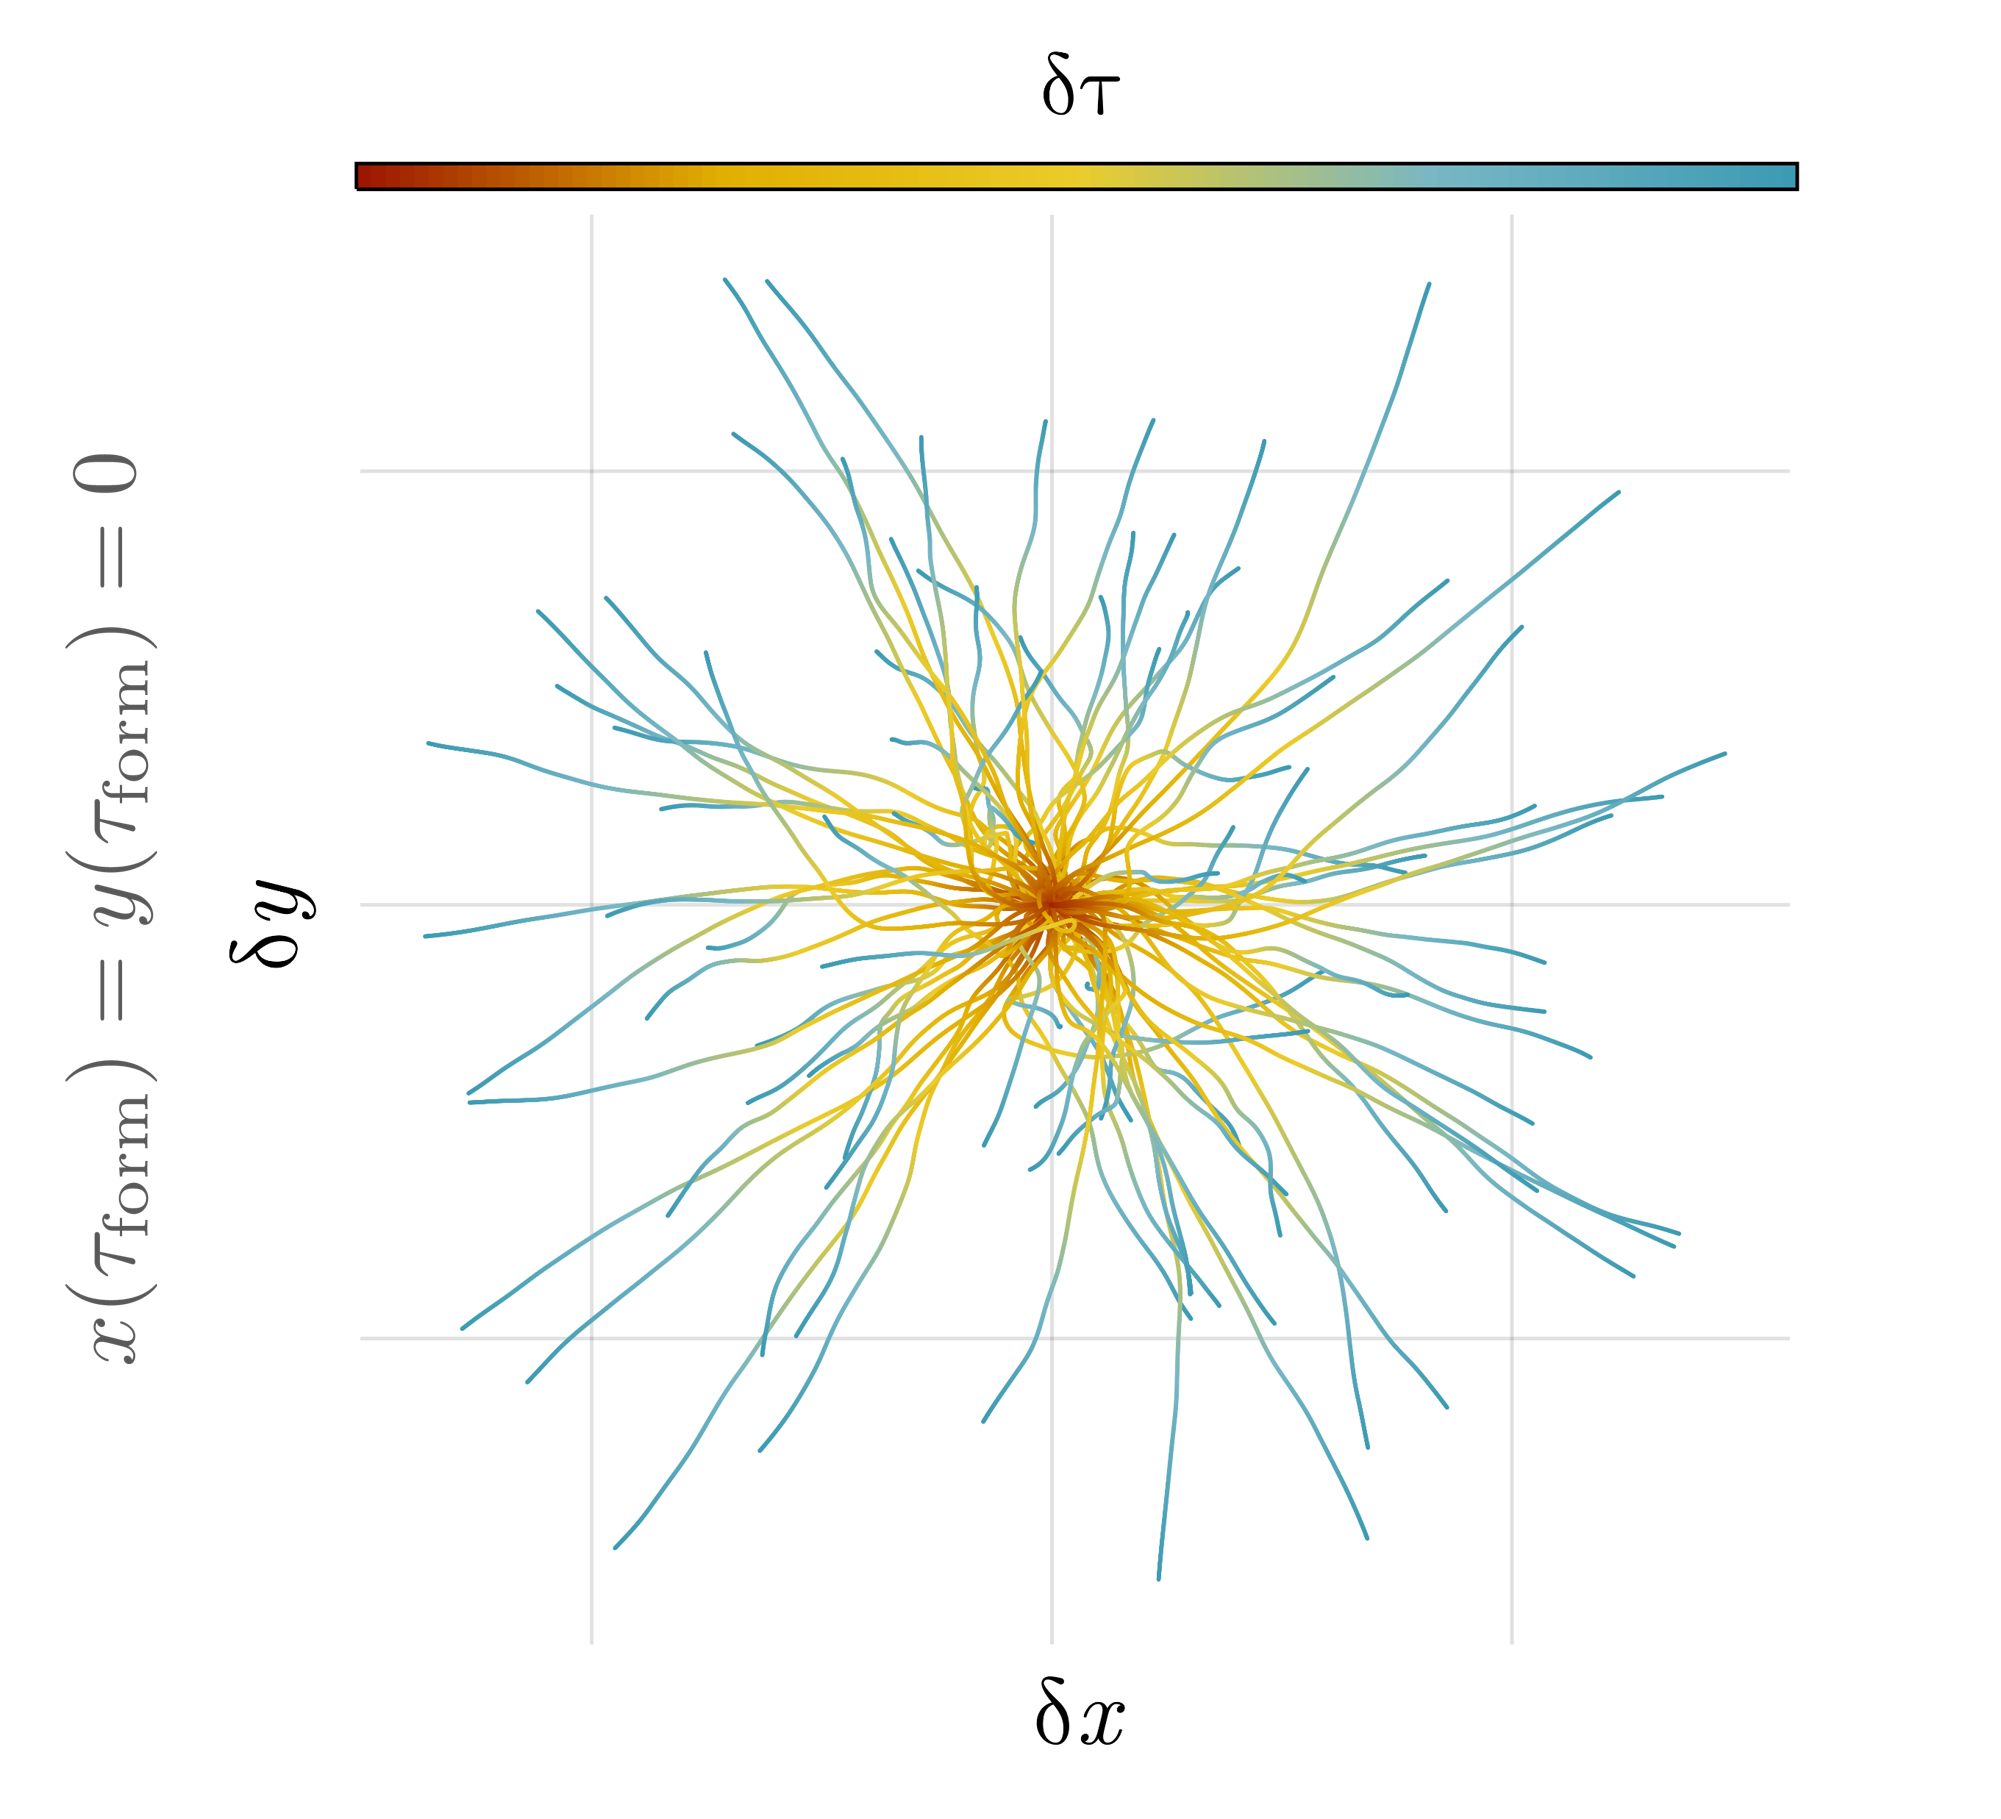
\includegraphics[width=1.1\columnwidth]{images/wong_coord.png}
                \end{figure}
                \column{.025\textwidth}
        \column{.3\textwidth}
            \begin{itemize}\itemsep0em 
                \setbeamertemplate{itemize item}{\raisebox{0.2em}{\scalebox{0.7}{${\color{normal}\blacktriangleright}$}}} 
                \item \begin{center}\footnotesize {\bfseries Momentum} broadening due to color Lorentz force\end{center}
            \end{itemize}
            \vspace{-20pt}
            \begin{figure}[!hbt]
                \centering
                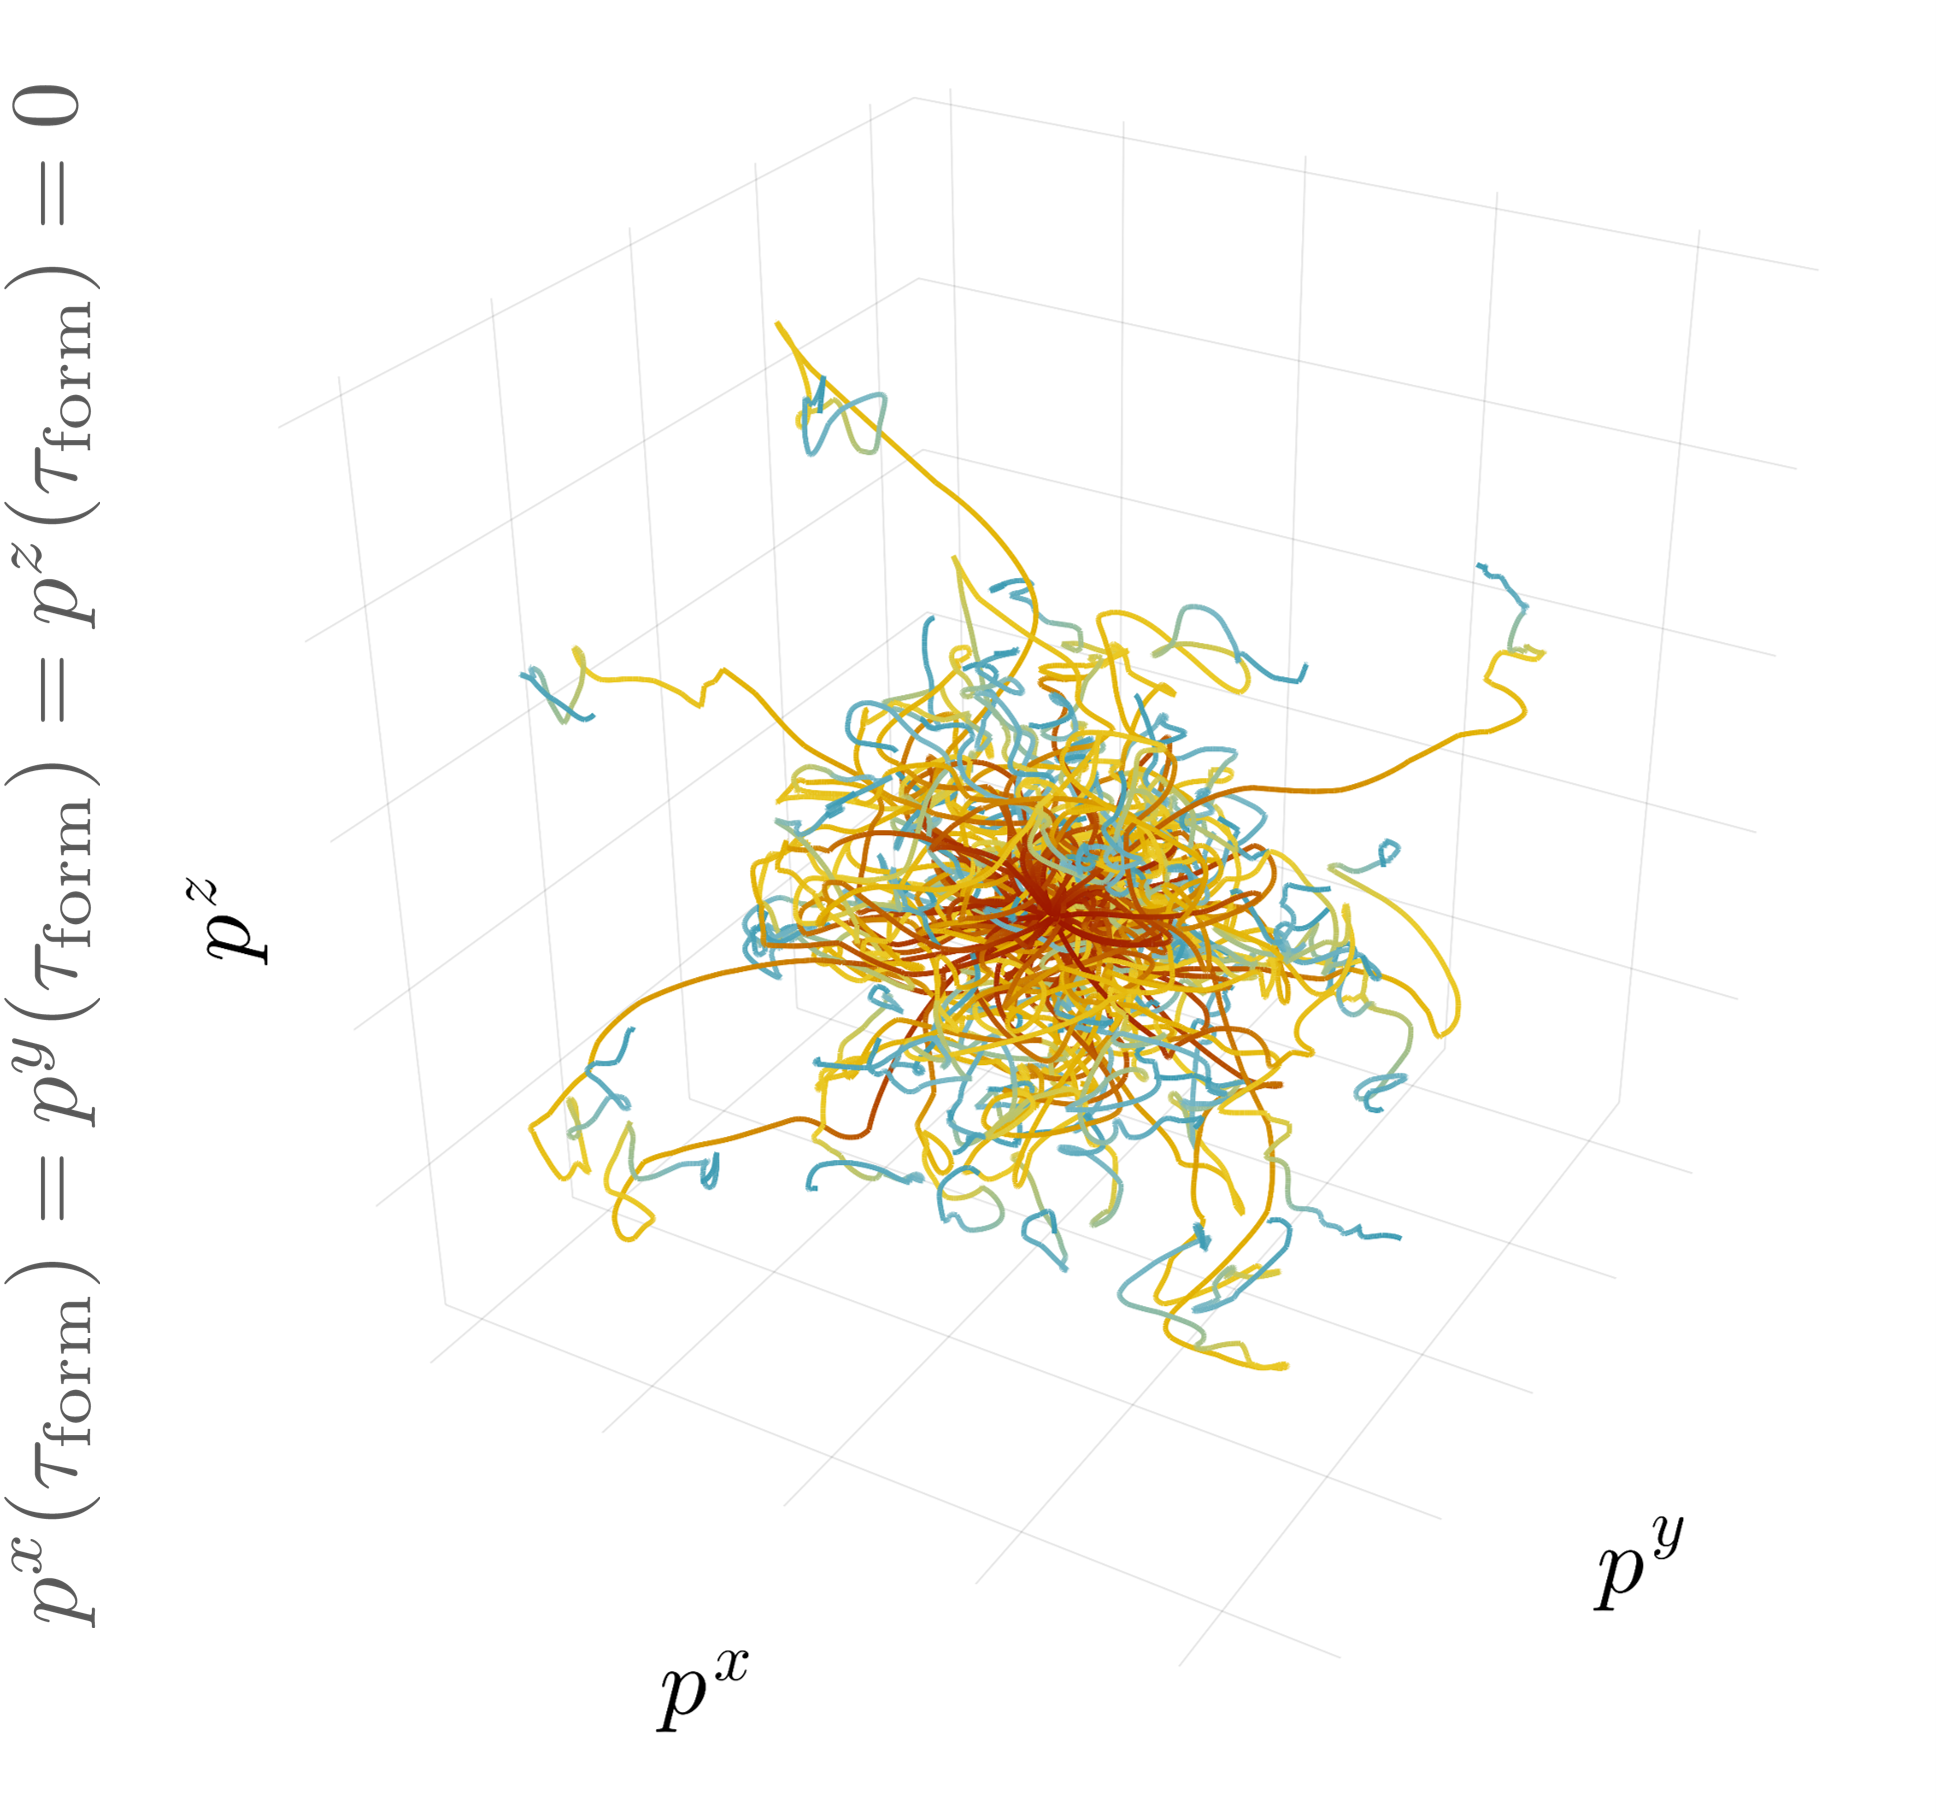
\includegraphics[width=1.1\columnwidth]{images/wong_mom.png}
            \end{figure}
            \column{.025\textwidth}
        \column{.3\textwidth}
            \begin{itemize}\itemsep0em 
                \setbeamertemplate{itemize item}{\raisebox{0.2em}{\scalebox{0.7}{${\color{normal}\blacktriangleright}$}}} 
                \item \begin{center}\footnotesize {\bfseries Color charge} rotation in SU(3) with Wilson lines\end{center}
            \end{itemize}
            \vspace{-15pt}
            \begin{figure}[!hbt]
                \centering
                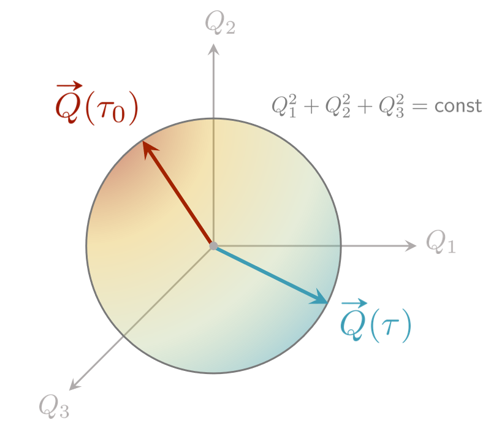
\includegraphics[width=1.05\columnwidth]{images/wong_charge.png}
            \end{figure}
            \column{.025\textwidth}
    \end{columns}

    \blfootnote{\scriptsize Avramescu, Băran, Greco, Ipp, Müller, Ruggieri  \href{https://arxiv.org/abs/2303.05599}{{\color{palgold}\texttt{[2303.05599]}$^\text{\tiny\faExternalLink}$}}}
\end{frame}


%%%%%%%%%%%%%%%%%%%%%%%%%%%%%%%%%%%%%%%%%
%%%%%%%%%%%%%%%% SECTION %%%%%%%%%%%%%%%%
%%%%%%%%%%%%%%%%%%%%%%%%%%%%%%%%%%%%%%%%%

\section{Observables}

\setbeamertemplate{background}{
\tikz[overlay,remember picture] \node[opacity=0.15, at=(current page.center)] {
   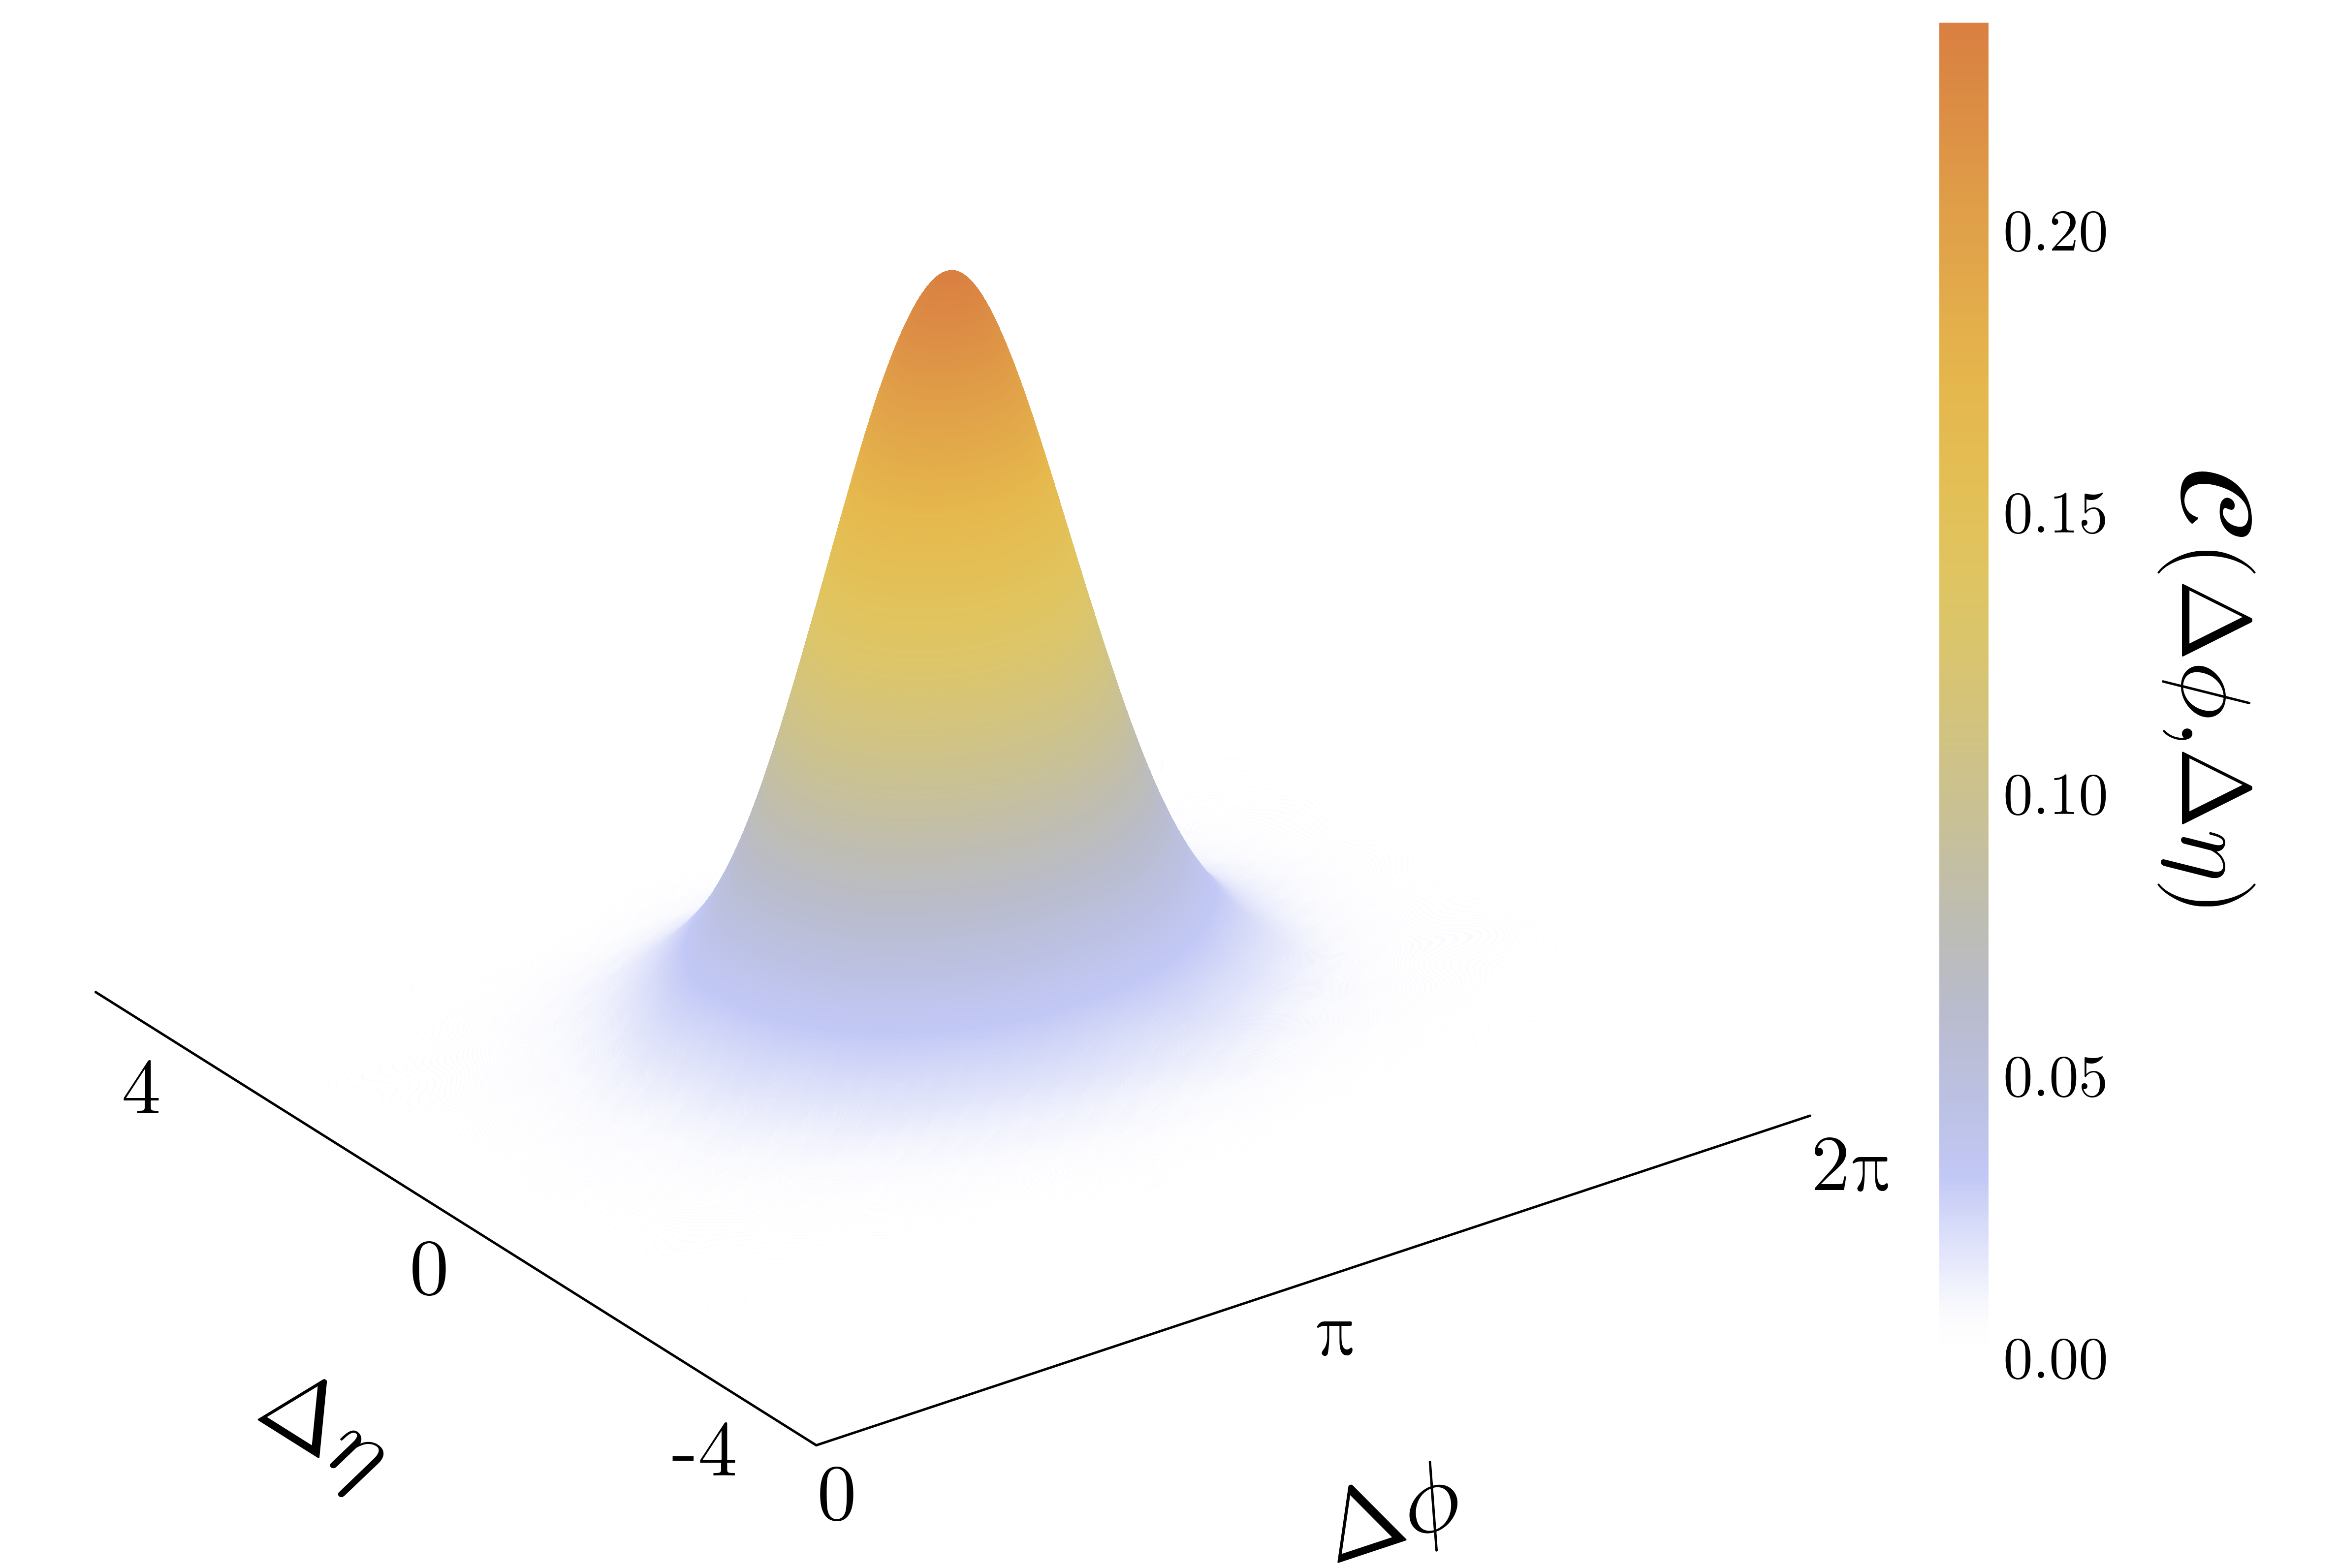
\includegraphics[height=0.8\paperheight]{images/Cdetadphi_3D_toy_charm_pT_1_tau_0.1_crop.png}};
}
\begin{frame}[plain,noframenumbering]{}
    \begin{center}
        \vspace{1cm}
        {\large\color{normal}How to probe pre-equilibrium}\\[0.3cm]
        {\huge\color{destacado}Seeking relevant observables}\\[0.4cm]
        {\large\textit{Candidates:} $R_{AA}$, $\mathcal{C}(\Delta\phi)$}
    \end{center}
\end{frame}
\setbeamertemplate{background}{}

%%%%%%%%%%%%%%%%%%%%%%%%%%%%%%%%%%%%%%%%%
%%%%%%%%%%%%%% SUBSECTION %%%%%%%%%%%%%%%
%%%%%%%%%%%%%%%%%%%%%%%%%%%%%%%%%%%%%%%%%

% \subsection{Nuclear modification factor}
\subsection{Spectra}

%%%%%%%%%%%%%%%%%%%%%%%%%%%%%%%%%%%%%%%%%
%%%%%%%%%%%%%%%%% SLIDE %%%%%%%%%%%%%%%%%
%%%%%%%%%%%%%%%%%%%%%%%%%%%%%%%%%%%%%%%%%

\begin{frame}
    \frametitle{Nuclear modification factor}
    % \framesubtitle{Extraction of $R_{AA}$ in glasma}
    \vspace{-10pt}
    \begin{columns}[onlytextwidth,t]
        \column{.033\textwidth}
        \column{.43\textwidth}
       \begin{center}
        \begin{custombox2}{$\boldsymbol{R_{AA}}$ in glasma}{lightgray}
            \small
            \begin{varwidth}{1.05\textwidth}
            \begin{itemize}\itemsep0em 
                \itemsep0em
                \setbeamertemplate{itemize item}{\raisebox{0.2em}{\scalebox{0.7}{${\color{lightgray}\blacktriangleright}$}}} 
                \item Ratio of ${\color{raapink}\boldsymbol{AA}}$ to ${\color{raablue}\boldsymbol{pp}}$ normalized spectra \\
                {\scriptsize\color{lightgray}${\color{raapink}\boldsymbol{AA}}$ evolved in {\color{raapink}\bfseries glasma}, ${\color{raablue}\boldsymbol{pp}}$ from {\color{raablue}\bfseries FONLL}}
            \end{itemize}
            \end{varwidth}
        \end{custombox2}

        % \begin{itemize}\itemsep0em 
        %     \itemsep0em
        %     \footnotesize\color{lightgray}
        %     \setbeamertemplate{itemize item}{\raisebox{0.2em}{\scalebox{0.7}{${\color{lightgray}\blacktriangleright}$}}} 
        %     \item ${\color{raapink}\boldsymbol{AA}}$ evolved in {\color{raapink}\bfseries glasma}, ${\color{raablue}\boldsymbol{pp}}$ from {\color{raablue}\bfseries FONLL} 
        %     % \item Glasma spectrum initialized with FONLL
        % \end{itemize}
        % \vspace{5pt}

        \begin{custombox2}{{\normalsize FONLL spectrum}}{raablue}
            \small
            \begin{varwidth}{1.05\textwidth}
            \begin{itemize}\itemsep0em 
                \itemsep0em
                \setbeamertemplate{itemize item}{\raisebox{0.2em}{\scalebox{0.7}{${\color{raablue}\blacktriangleright}$}}} 
                \footnotesize
                \item Initial pQCD $p_T$ spectrum for bare quarks\\
                {\scriptsize\color{lightgray}Fixed-Order+Next-to-Leading Logarithm}
            \end{itemize}
            \end{varwidth}
        \end{custombox2}

        \renewcommand{\eqnhighlightheight}{\vphantom{\mathcal{D}_\mu}\mathstrut}
        \begin{equation*}
            \hspace{0pt}
            R_{AA}(\boldsymbol{\textcolor{palteal}\tau})=\dfrac{1}{A^2}\dfrac{{\color{palteal}\sigma}^{\textcolor{normal}{AA}}_{\mathrm{\textcolor{palteal}{tot}}}}{\eqnmark[palteal]{sigma}{{\color{palteal}\sigma}^{\textcolor{normal}{pp}}_{\mathrm{\textcolor{palteal}{tot}}}}}\dfrac{\eqnmark[raapink]{gl}{\mathrm{d}N/\mathrm{d}p_T}(\boldsymbol{\textcolor{palteal}\tau})}{\eqnmark[raablue]{fonll}{\mathrm{d}N^{pp}/\mathrm{d}p_T}}
        \end{equation*}
        \annotate[yshift=-0.5em]{below, left}{sigma}{\tiny normalization}
        \annotate[yshift=0.7em]{above, left}{gl}{\tiny glasma}
        \annotate[yshift=-0.5em]{below, left}{fonll}{\tiny FONLL}

       \end{center}
       \column{.033\textwidth}
       \column{.47\textwidth}
       \begin{center}
        \begin{custombox2}{\normalsize Time $\boldsymbol{\tau}$ evolution}{palteal}
            \small
            \begin{varwidth}{0.88\textwidth}
            \begin{itemize}\itemsep0em 
                \itemsep0em
                \footnotesize
                \setbeamertemplate{itemize item}{\raisebox{0.2em}{\scalebox{0.7}{${\color{palteal}\blacktriangleright}$}}} 
                \item More enhancement in $R_{AA}$ at later $\tau$
            \end{itemize}
            \end{varwidth}
        \end{custombox2}
    \end{center}
        \vspace{-10pt}
           \begin{figure}
                \centering
                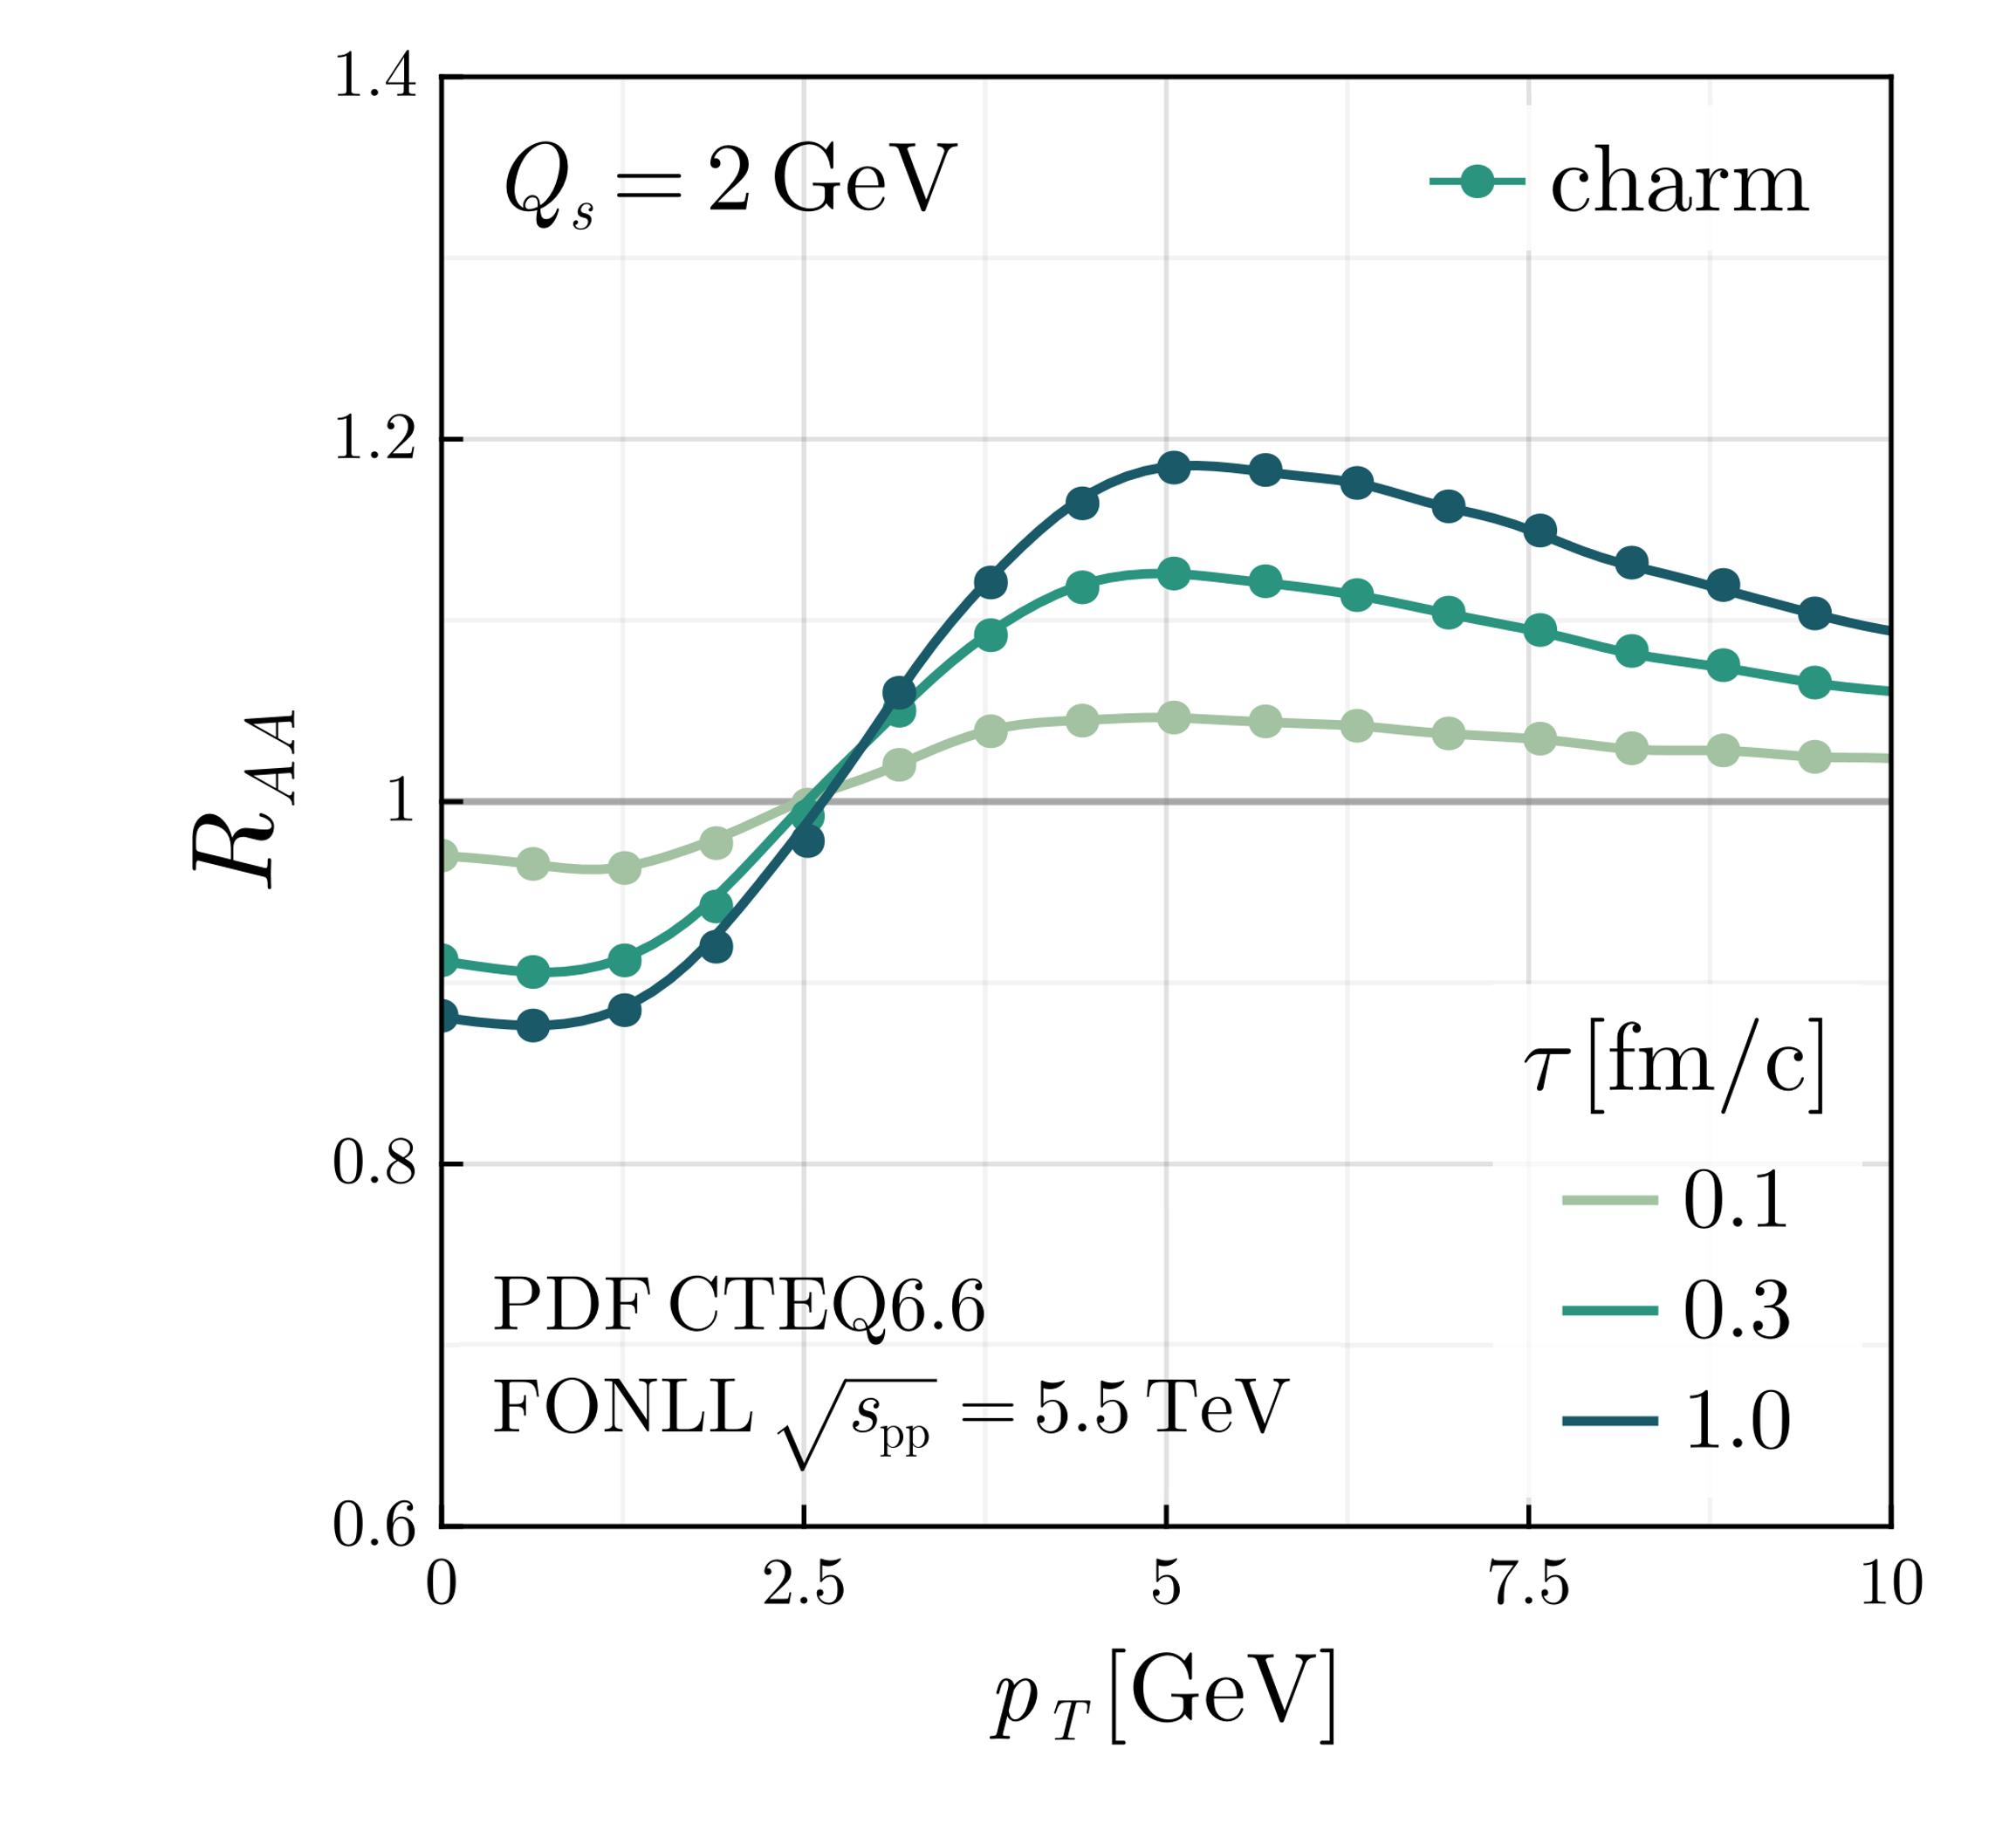
\includegraphics[width=0.9\columnwidth]{images/clean_raa_tau_dep_quarks_charmQs_2.0_fonll_energy_5500_pdf_cteq.png}
            \end{figure}
       
        \column{.033\textwidth}
    \end{columns}

    \vspace{-20pt}
    \blfootnote{\scriptsize Cacciari, Greco, Nason \href{https://arxiv.org/abs/hep-ph/9803400}{{\color{raablue}\texttt{[hep-ph/9803400]$^\text{\tiny\faExternalLink}$}}}, \href{https://www.lpthe.jussieu.fr/~cacciari/fonll/fonllform.html}{{\color{raablue}\texttt{[FONLL web form]$^\text{\tiny\faLink}$}}}}
\end{frame}


%%%%%%%%%%%%%%%%%%%%%%%%%%%%%%%%%%%%%%%%%
%%%%%%%%%%%%%%%%% SLIDE %%%%%%%%%%%%%%%%%
%%%%%%%%%%%%%%%%%%%%%%%%%%%%%%%%%%%%%%%%%

\begin{frame}
    \frametitle{$R_{AA}$ in glasma with nPDFs}
    % \framesubtitle{Temporal evolution, energy dependence}
    \vspace{-15pt}
    \begin{center}
        \begin{columns}[onlytextwidth,t]
            \column{.02\textwidth}
           \column{.47\textwidth}
           \begin{center}
                \begin{custombox2}{\normalsize Previous studies}{raablue}
                    \small
                    \begin{varwidth}{0.88\textwidth}
                    \begin{itemize}\itemsep0em 
                        \itemsep0em
                        \footnotesize
                        \setbeamertemplate{itemize item}{\raisebox{0.2em}{\scalebox{0.7}{${\color{raablue}\blacktriangleright}$}}} 
                        \item $AA$ glasma spectrum initialized with FONLL in $pp$, {\bfseries\color{raablue}no nPDF effect}
                    \end{itemize}
                    \end{varwidth}
                \end{custombox2}
                \begin{untitledcustombox}
                    \begin{varwidth}{0.88\textwidth}
                        \hspace{10pt}\normalsize{\bfseries\color{palteal} This study}: FONLL + {\color{palteal}EPPS16}\hspace{10pt}
                    \end{varwidth}
                \end{untitledcustombox}
            \end{center}
                % something
            % \end{custombox3}
            \vspace{-20pt}
            \begin{center}
                \begin{tikzpicture}[]
                    \node[anchor=south west,inner sep=0] at (0,0) {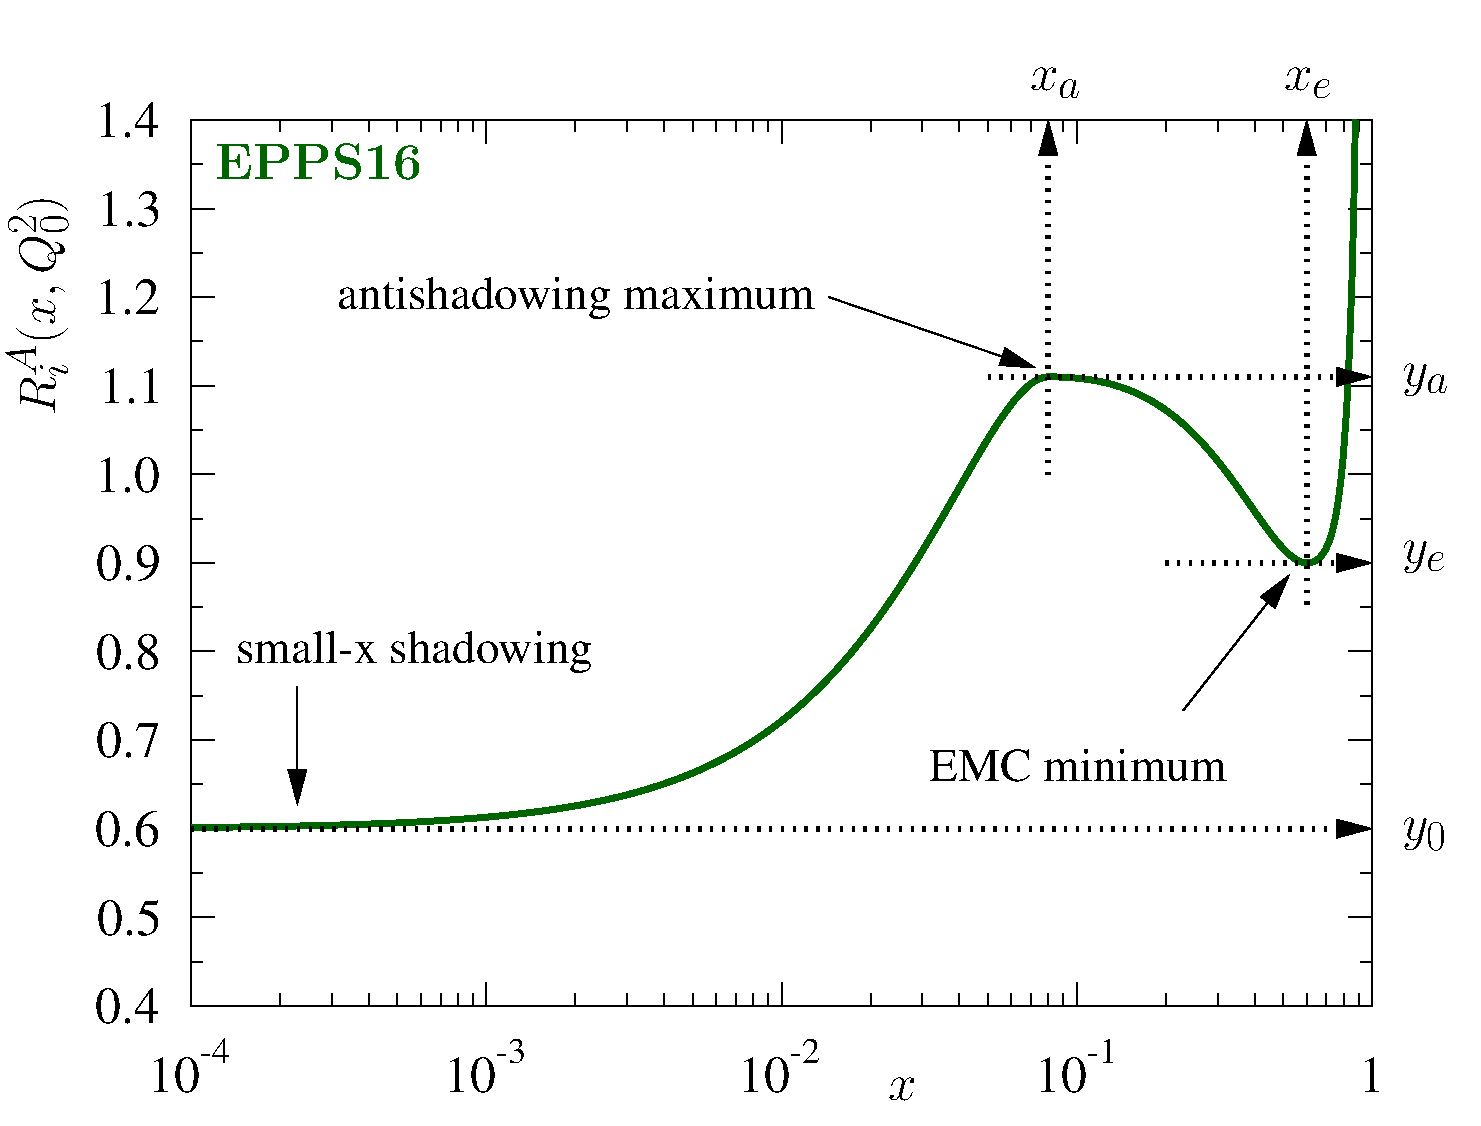
\includegraphics[width=0.75\columnwidth]{images/FitForm_EPPS16.pdf}};
                    \draw<1>[palteal,line width=1pt,fill=palteal,fill opacity=0.1,rounded corners=2pt] (0.685, 0.44) rectangle (2.5, 3.65);
                \end{tikzpicture}
            \end{center}
        %    \begin{figure}
        %         \centering
        %         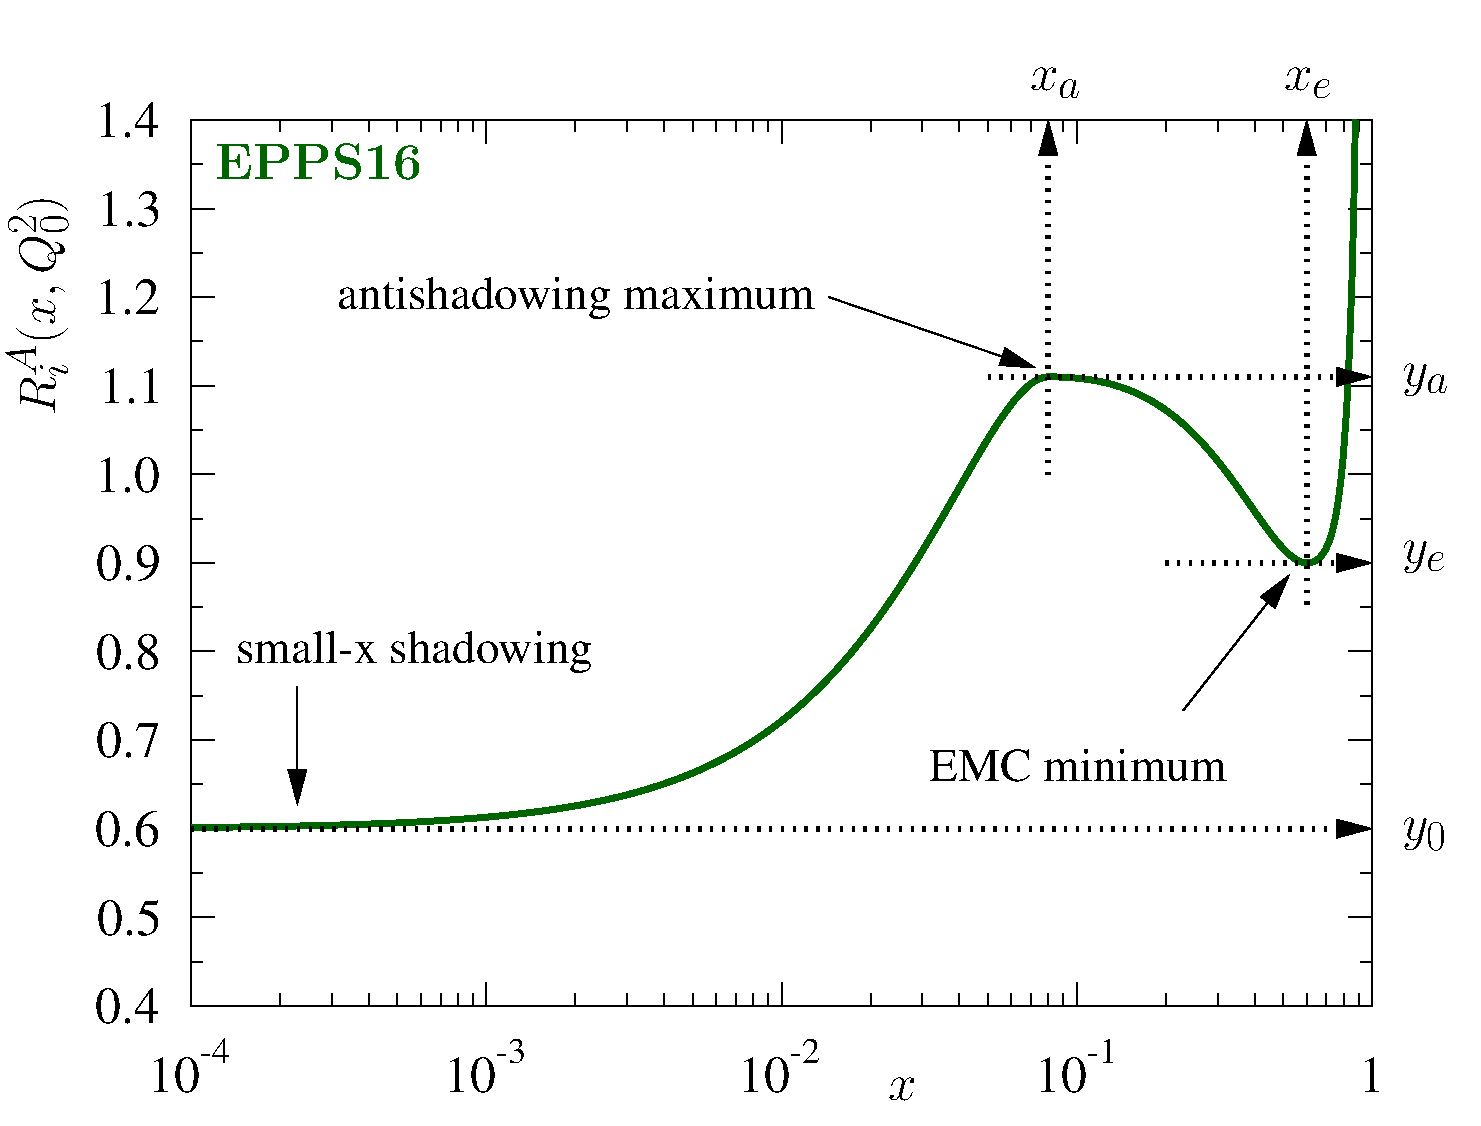
\includegraphics[width=0.75\columnwidth]{images/FitForm_EPPS16.pdf}
        %     \end{figure}
            \column{.02\textwidth}
            \column{.47\textwidth}
            \begin{center}
                \begin{custombox2}{\normalsize nPDF + glasma}{palgold}
                    \small
                    \begin{varwidth}{0.95\textwidth}
                    \begin{itemize}\itemsep0em 
                        \itemsep0em
                        \footnotesize
                        \setbeamertemplate{itemize item}{\raisebox{0.2em}{\scalebox{0.7}{${\color{palgold}\blacktriangleright}$}}} 
                        \item Glasma effect modest compared to nPDF
                    \end{itemize}
                    \end{varwidth}
                \end{custombox2}
            \end{center}
            \vspace{-18pt}
            \begin{figure}
                \centering
                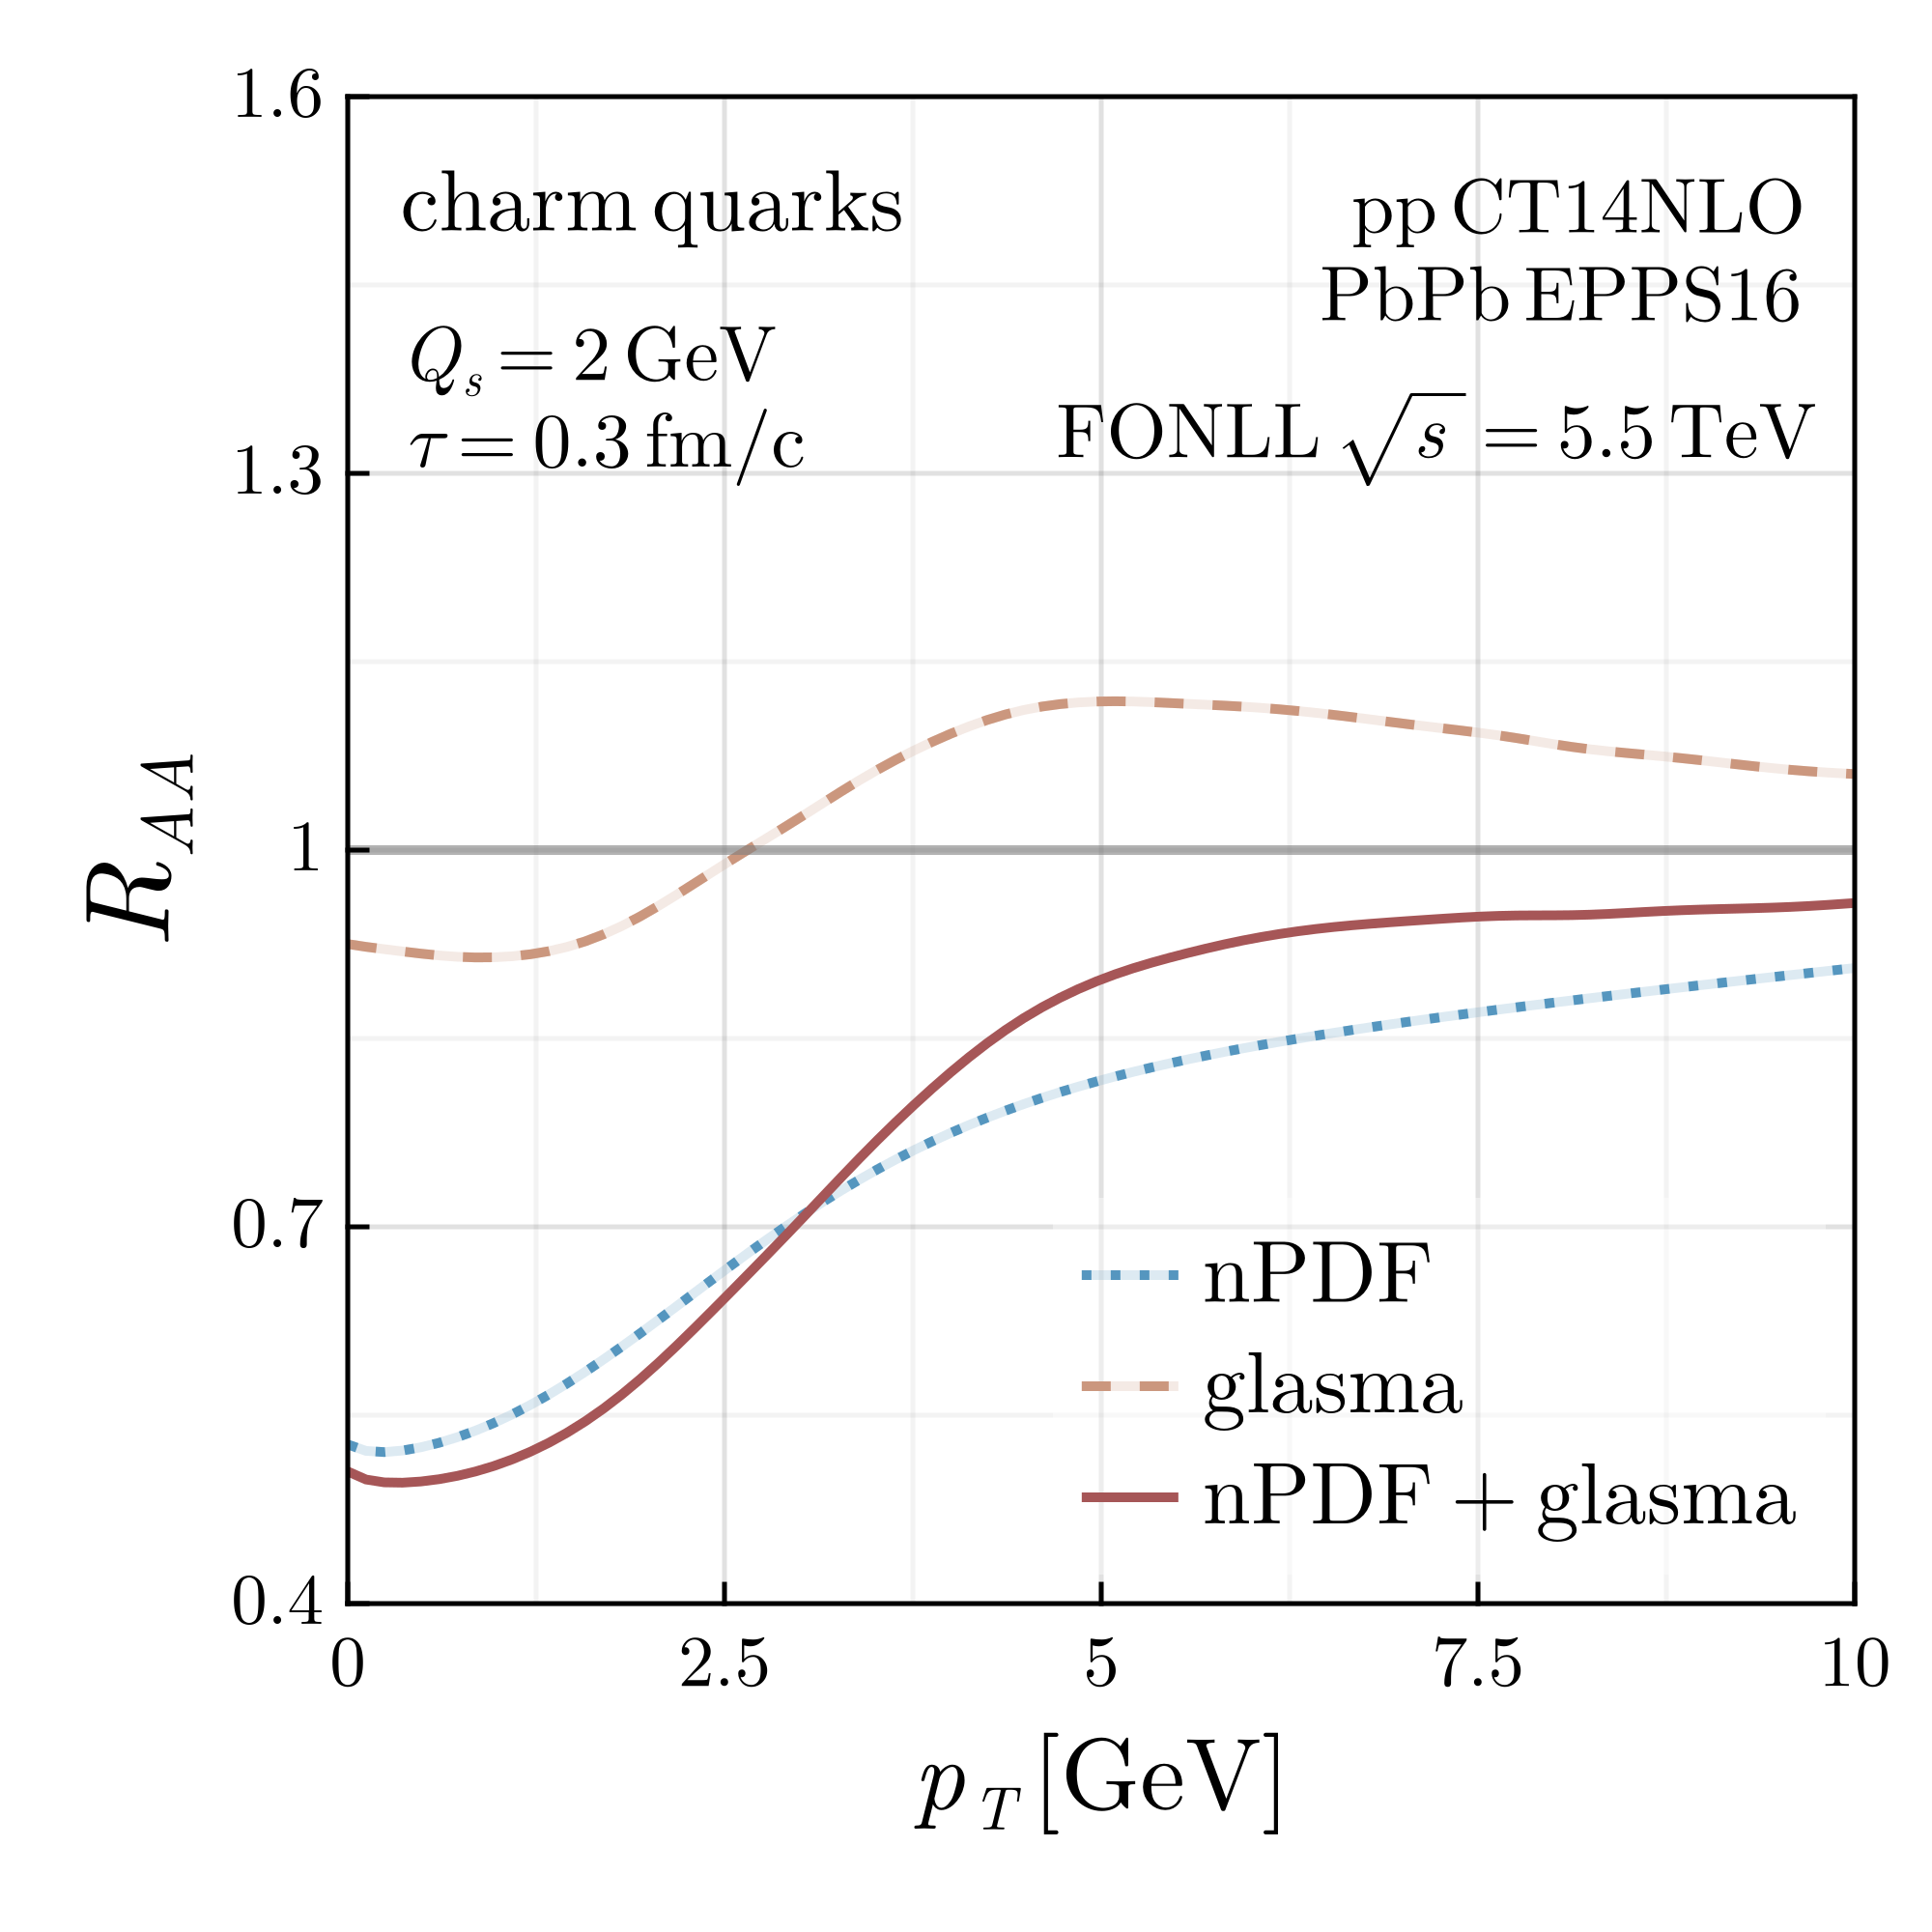
\includegraphics[width=0.82\columnwidth]{images/clean_raa_tau_0.3_charm_quark_Qs_2.0_fonll_pdf_vs_npdf_v3.png}
            \end{figure}
            \column{.02\textwidth}
        \end{columns}    
    \end{center}
    \vspace{-25pt}
    \blfootnote{\scriptsize Sun, Coci, Das, Plumari, Ruggieri, Greco \href{https://arxiv.org/abs/1902.06254}{{\color{raablue}\texttt{[1902.06254]$^\text{\tiny\faExternalLink}$}}}\\
    \hspace{14pt} Eskola, Paakkinen, Paukkunen, Salgado \href{https://arxiv.org/abs/1612.05741}{{\color{palteal}\texttt{[1612.05741]$^\text{\tiny\faExternalLink}$}}}}
\end{frame}

%%%%%%%%%%%%%%%%%%%%%%%%%%%%%%%%%%%%%%%%%
%%%%%%%%%%%%%%%%% SLIDE %%%%%%%%%%%%%%%%%
%%%%%%%%%%%%%%%%%%%%%%%%%%%%%%%%%%%%%%%%%

\begin{frame}[noframenumbering]
    \frametitle{$R_{AA}$ in glasma}
    % \framesubtitle{Temporal evolution, energy dependence}
    {\transparent{0.1}\vspace{-15pt}
    \begin{center}
        \begin{columns}[onlytextwidth,t]
            \column{.02\textwidth}
           \column{.47\textwidth}
           \begin{center}
                \begin{custombox2transp}{\normalsize\transparent{0.1} Previous studies}{raablue}
                    \small
                    \begin{varwidth}{0.88\textwidth}
                    \begin{itemize}\itemsep0em 
                        \itemsep0em
                        \footnotesize
                        \setbeamertemplate{itemize item}{\raisebox{0.2em}{\scalebox{0.7}{${\color{raablue}\blacktriangleright}$}}} 
                        \item \transparent{0.1}$AA$ glasma spectrum initialized with FONLL in $pp$, {\bfseries\color{raablue}no nPDF effect}
                    \end{itemize}
                    \end{varwidth}
                \end{custombox2transp}
                \begin{untitledcustomboxtransp}
                    \begin{varwidth}{0.88\textwidth}
                        \hspace{10pt}\normalsize{\bfseries\color{palteal} \transparent{0.1}This study}: FONLL + {\color{palteal}EPPS16}\hspace{10pt}
                    \end{varwidth}
                \end{untitledcustomboxtransp}
            \end{center}
                % something
            % \end{custombox3}
            \vspace{-20pt}
            \begin{center}
                \begin{tikzpicture}[]
                    \node[anchor=south west,inner sep=0] at (0,0) {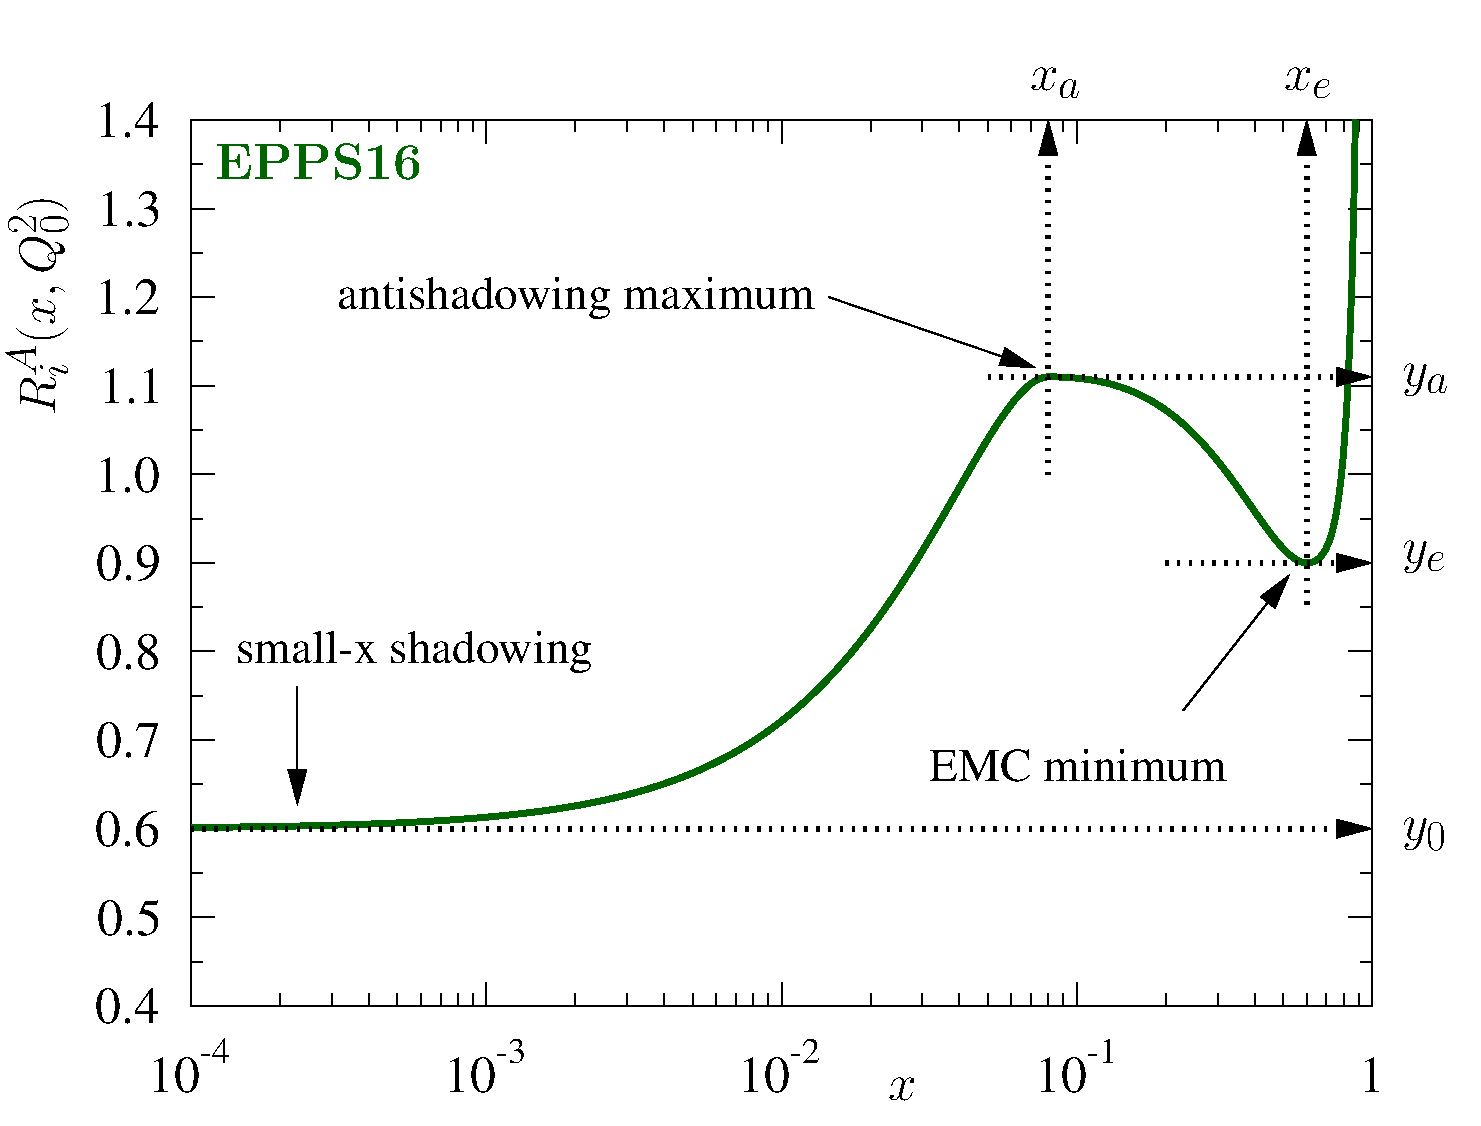
\includegraphics[width=0.75\columnwidth]{images/FitForm_EPPS16.pdf}};
                    \draw<1>[palteal,line width=1pt,fill=palteal,fill opacity=0.02,rounded corners=2pt] (0.685, 0.44) rectangle (2.5, 3.65);
                \end{tikzpicture}
            \end{center}
        %    \begin{figure}
        %         \centering
        %         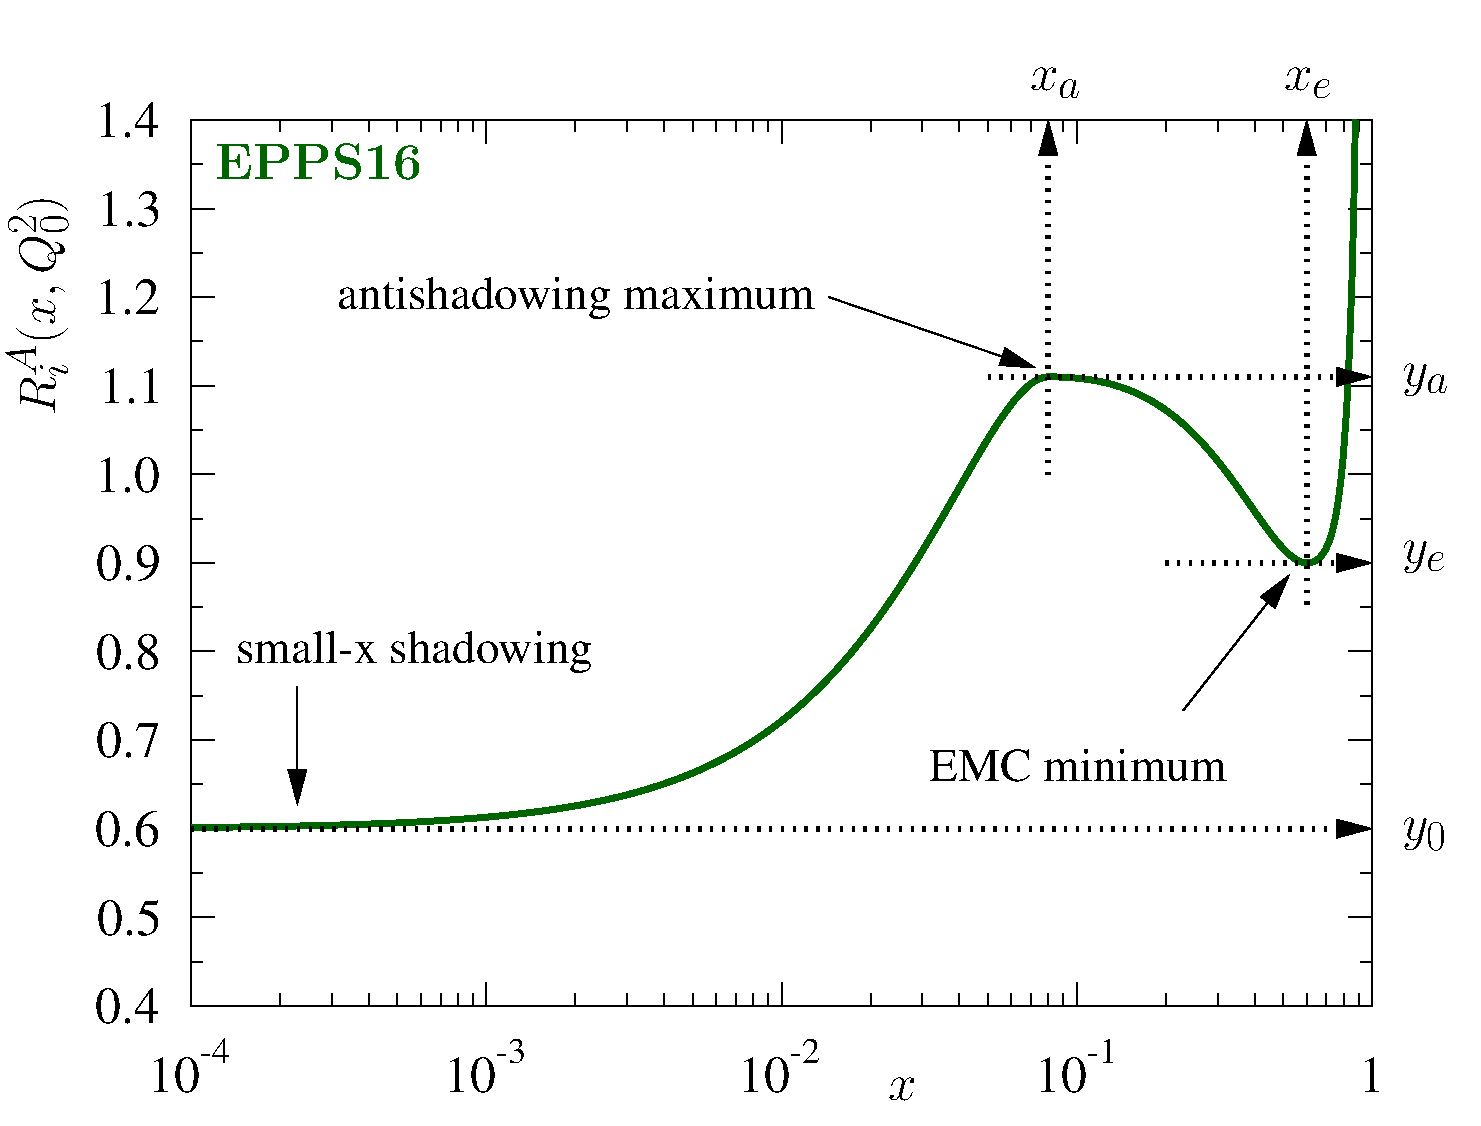
\includegraphics[width=0.75\columnwidth]{images/FitForm_EPPS16.pdf}
        %     \end{figure}
            \column{.02\textwidth}
            \column{.47\textwidth}
            \begin{center}
                \begin{custombox2transp}{\normalsize \transparent{0.1}nPDF + glasma}{palgold}
                    \small
                    \begin{varwidth}{0.95\textwidth}
                    \begin{itemize}\itemsep0em 
                        \itemsep0em
                        \footnotesize
                        \setbeamertemplate{itemize item}{\raisebox{0.2em}{\scalebox{0.7}{${\color{palgold}\blacktriangleright}$}}} 
                        \item \transparent{0.1}Glasma effect modest compared to nPDF
                    \end{itemize}
                    \end{varwidth}
                \end{custombox2transp}
            \end{center}
            \vspace{-18pt}
            \begin{figure}
                \centering
                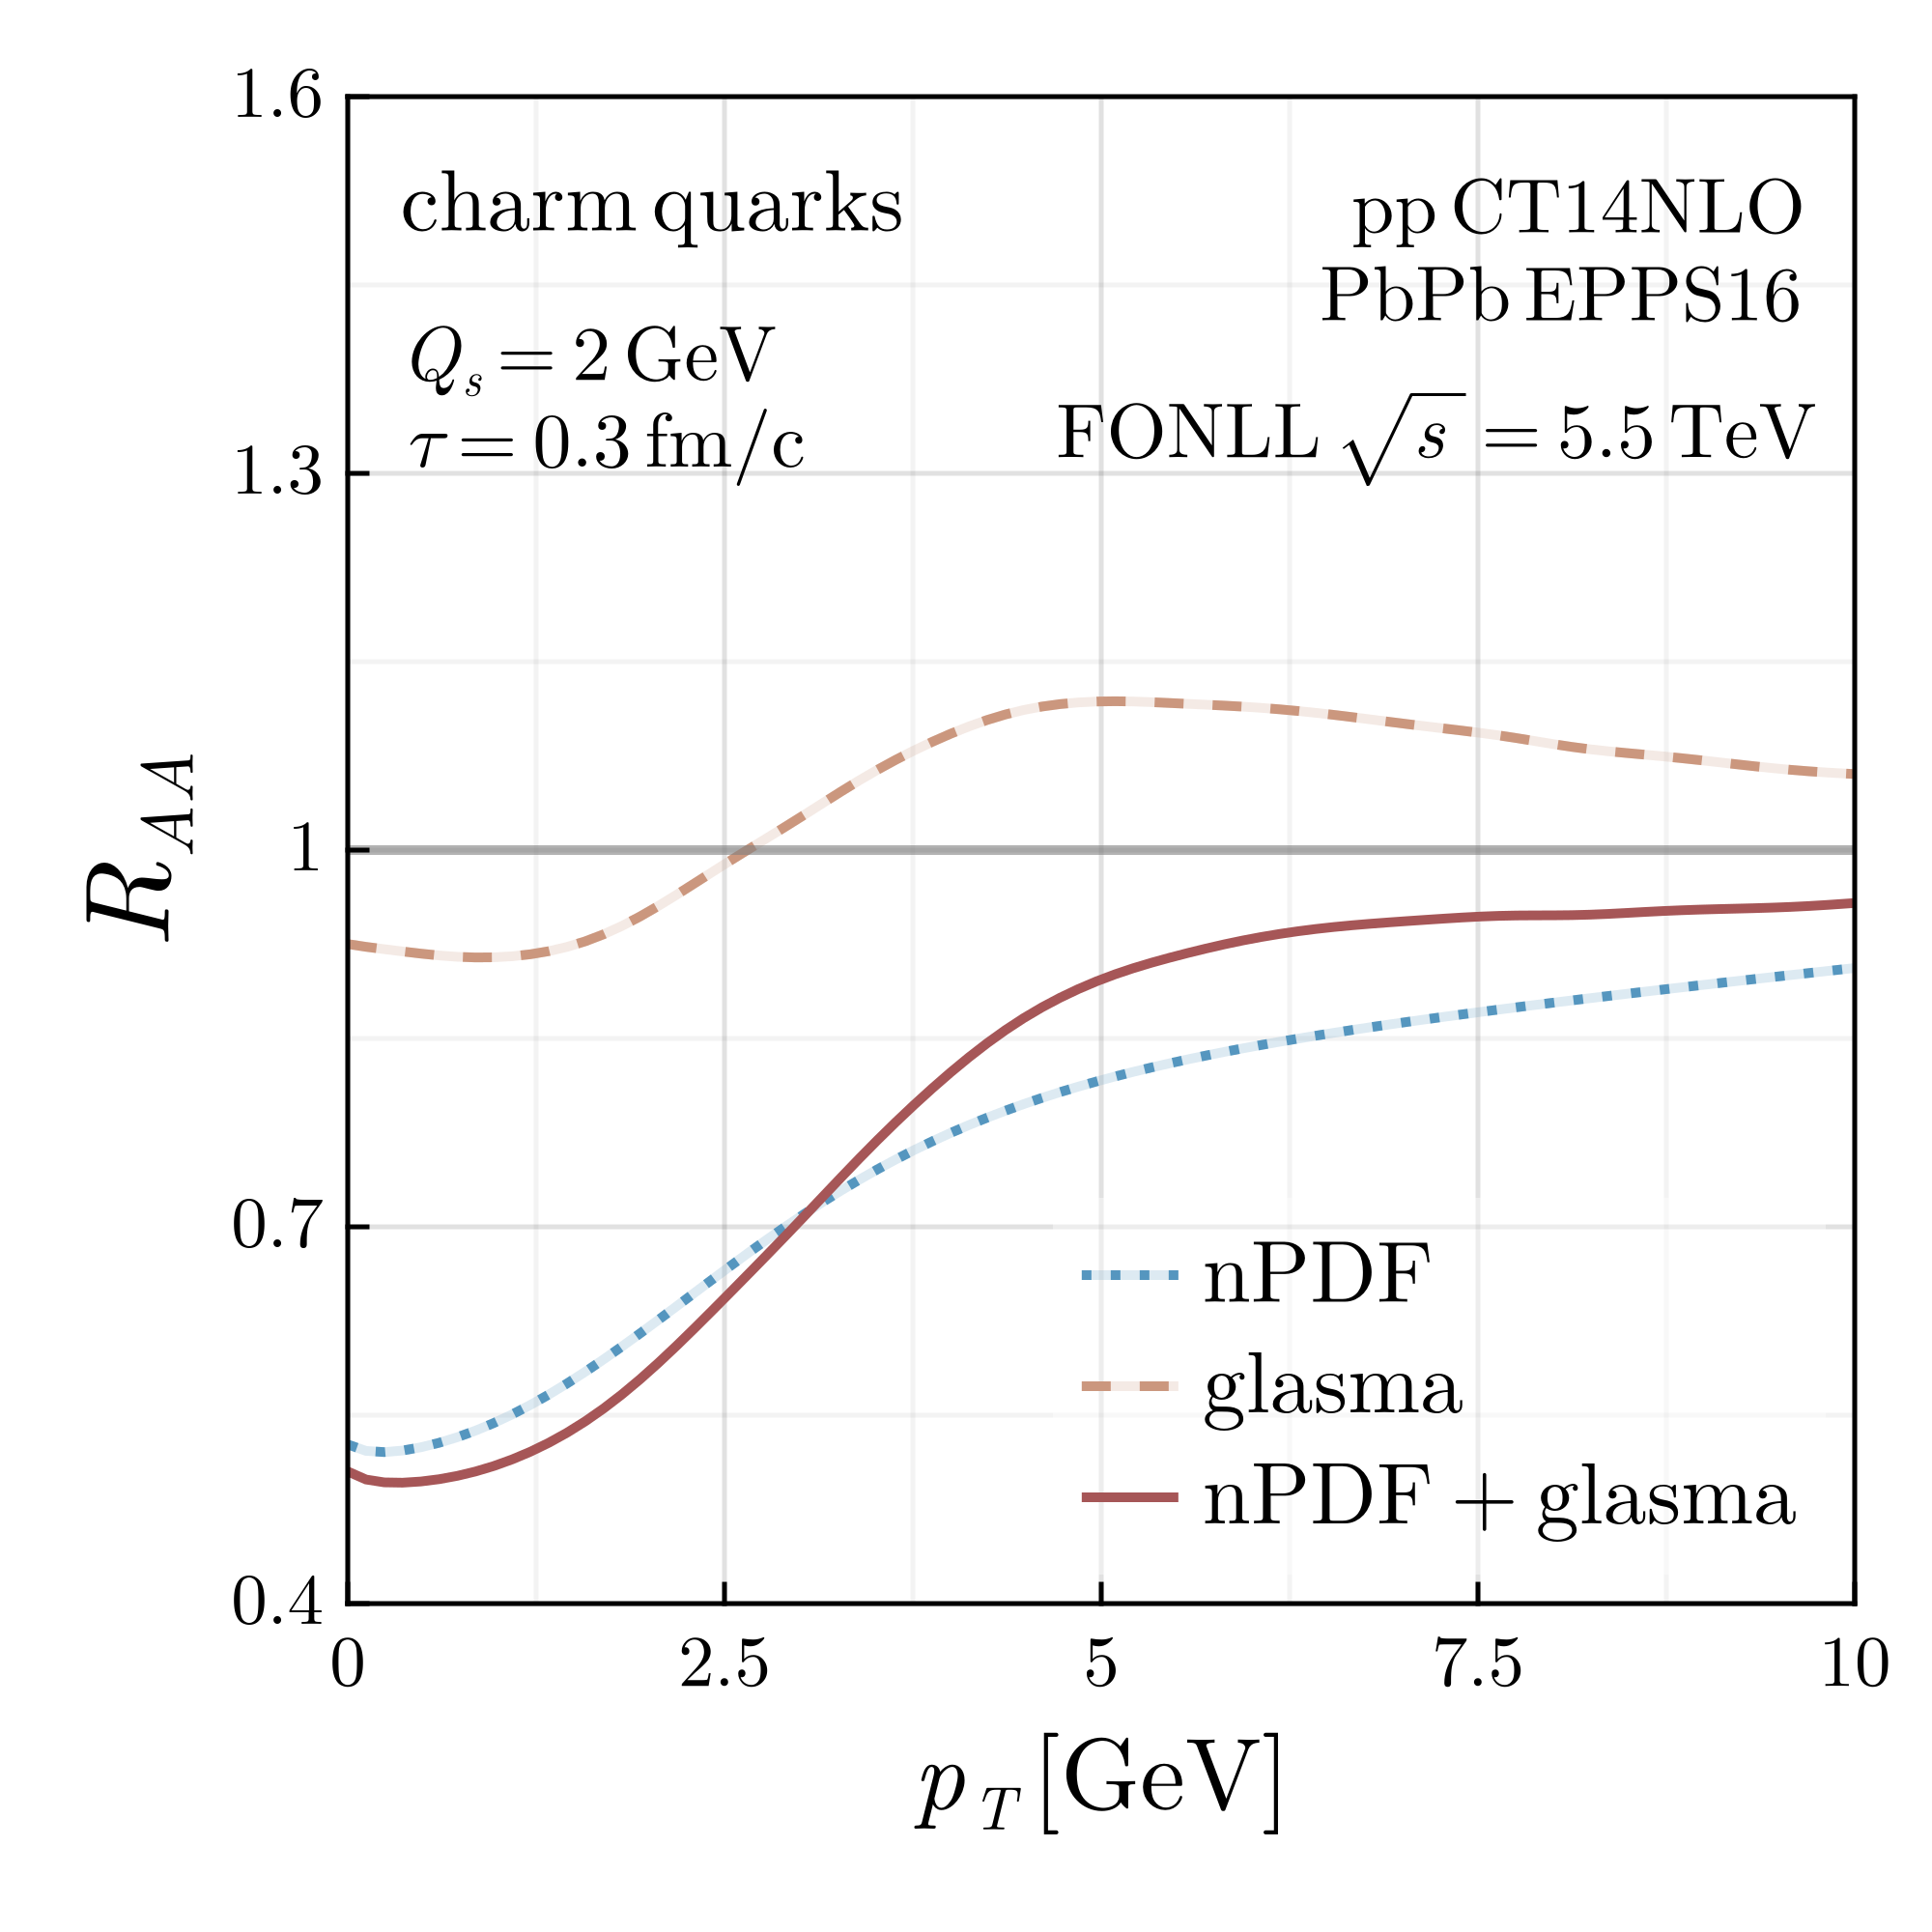
\includegraphics[width=0.82\columnwidth]{images/clean_raa_tau_0.3_charm_quark_Qs_2.0_fonll_pdf_vs_npdf_v3.png}
            \end{figure}
            \column{.02\textwidth}
        \end{columns}    
    \end{center}
    % \vspace{-25pt}
    % \blfootnote{\scriptsize Sun, Coci, Das, Plumari, Ruggieri, Greco \href{https://arxiv.org/abs/1902.06254}{{\color{raablue}\texttt{[1902.06254]$^\text{\tiny\faExternalLink}$}}}\\
    % \hspace{14pt} Eskola, Paakkinen, Paukkunen, Salgado \href{https://arxiv.org/abs/1612.05741}{{\color{palteal}\texttt{[1612.05741]$^\text{\tiny\faExternalLink}$}}}}
    }

    \begin{center}
        \vspace{-10pt}
        \begin{tikzpicture}[remember picture,overlay]
            \node[align=center] at (0,4) {
                \large \textit{Candidate observable}\\[5pt]
                \huge Heavy quark $R_{AA}$\\[15pt]
                \Large Glasma causes {\color{palgold}$p_T$ migration}\\[7pt]
                \Large {\color{palgold}Weak effect} compared to nPDF 
            };
        \end{tikzpicture} 
    \end{center}
\end{frame}

%%%%%%%%%%%%%%%%%%%%%%%%%%%%%%%%%%%%%%%%%
%%%%%%%%%%%%%% SUBSECTION %%%%%%%%%%%%%%%
%%%%%%%%%%%%%%%%%%%%%%%%%%%%%%%%%%%%%%%%%

% \subsection{Two-particle correlations}
\subsection{Correlations}

%%%%%%%%%%%%%%%%%%%%%%%%%%%%%%%%%%%%%%%%%
%%%%%%%%%%%%%%%%% SLIDE %%%%%%%%%%%%%%%%%
%%%%%%%%%%%%%%%%%%%%%%%%%%%%%%%%%%%%%%%%%

\begin{frame}
    \frametitle{Two-particle correlations}
    \framesubtitle{$Q\overline{Q}$ pairs evolving in glasma}
    \vspace{-15pt}
    \begin{center}
        \begin{columns}[onlytextwidth,t]
            \column{.02\textwidth}
           \column{.47\textwidth}
           \begin{center}
                \begin{custombox2}{\normalsize Simulation setup}{lightgray}
                    \small
                    \begin{varwidth}{\textwidth}
                    \begin{itemize}\itemsep0em 
                        \itemsep0em
                        \footnotesize
                        \setbeamertemplate{itemize item}{\raisebox{0.2em}{\scalebox{0.7}{${\color{lightgray}\blacktriangleright}$}}} 
                        \item $Q\overline{Q}$ pairs produced {\bfseries back-to-back} (LO) in $\boldsymbol{\phi}$
                    \end{itemize}
                    \end{varwidth}
                \end{custombox2}
            \end{center}
            \column{.02\textwidth}
            \column{.47\textwidth}
            \begin{center}
                \begin{custombox2}{\normalsize Control parameters}{palviolet}
                    \small
                    \begin{varwidth}{0.95\textwidth}
                    \begin{itemize}\itemsep0em 
                        \itemsep0em
                        \footnotesize
                        \setbeamertemplate{itemize item}{\raisebox{0.2em}{\scalebox{0.7}{${\color{palviolet}\blacktriangleright}$}}} 
                        \item Glasma field {\color{palviolet}$\boldsymbol{Q_s}$} + heavy quark initial {\color{palviolet}$\boldsymbol{p_T}$}
                    \end{itemize}
                    \end{varwidth}
                \end{custombox2}
            \end{center}
            \column{.02\textwidth}
        \end{columns}    

        \begin{figure}
            \centering
            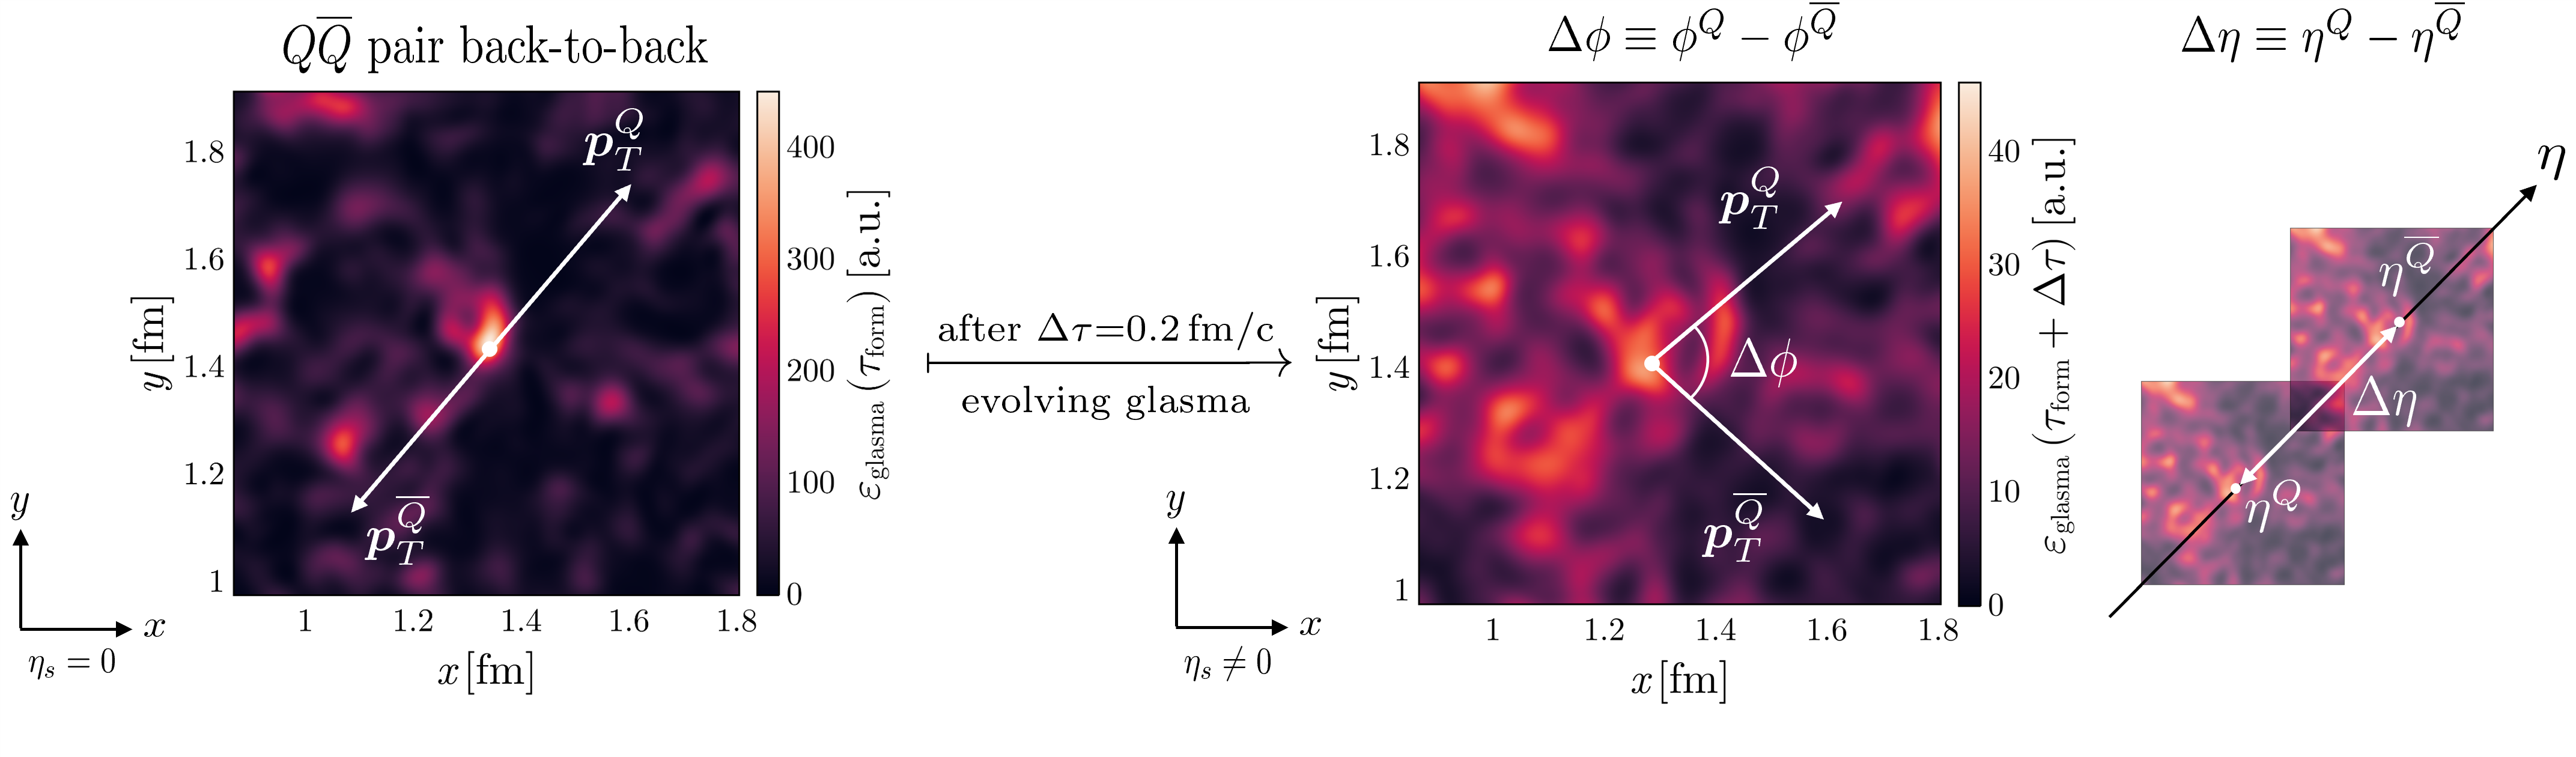
\includegraphics[width=0.95\columnwidth]{images/sketch_quark_pair_evo_final.png}
        \end{figure}
    \end{center}
\end{frame}

%%%%%%%%%%%%%%%%%%%%%%%%%%%%%%%%%%%%%%%%%
%%%%%%%%%%%%%%%%% SLIDE %%%%%%%%%%%%%%%%%
%%%%%%%%%%%%%%%%%%%%%%%%%%%%%%%%%%%%%%%%%

\begin{frame}
    \frametitle{Decorrelation of $Q\overline{Q}$ pairs}
    \framesubtitle{Quantifying the decorrelation in glasma}
    \vspace{-15pt}
    \begin{center}
        \begin{columns}[onlytextwidth,t]
            \column{.02\textwidth}
           \column{.58\textwidth}
           \begin{center}
                \begin{custombox2}{\normalsize Decorrelation in glasma}{lightgray}
                    \small
                    \begin{varwidth}{1.02\textwidth}
                    \begin{itemize}\itemsep0em 
                        \itemsep0em
                        \footnotesize
                        \setbeamertemplate{itemize item}{\raisebox{0.2em}{\scalebox{0.7}{${\color{lightgray}\blacktriangleright}$}}} 
                        \item Two-particle correlations $\boldsymbol{\mathcal{C}(\Delta\phi, \Delta\eta)}$ at $\boldsymbol{\Delta\tau}=\tau-\tau_\mathrm{form}$
                        \item Initial peak $\delta(\Delta\phi-\pi)\delta(\Delta\eta)$ gets broadened by glasma
                    \end{itemize}
                    \end{varwidth}
                \end{custombox2}
                % \begin{itemize}\itemsep0em 
                %     \itemsep0em
                %     \footnotesize\color{lightgray}
                %     \setbeamertemplate{itemize item}{\raisebox{0.2em}{\scalebox{0.7}{${\color{lightgray}\blacktriangleright}$}}} 
                %     \item Two-particle correlations extracted as\\
                %     $\mathcal{C}(\Delta\phi, \Delta\eta)=\dfrac{1}{N_\mathrm{pairs}}\dfrac{\mathrm{d}^2N}{\mathrm{d}\Delta\phi\mathrm{d}\Delta\eta}$
                % \end{itemize}

                \begin{figure}
                    \centering
                    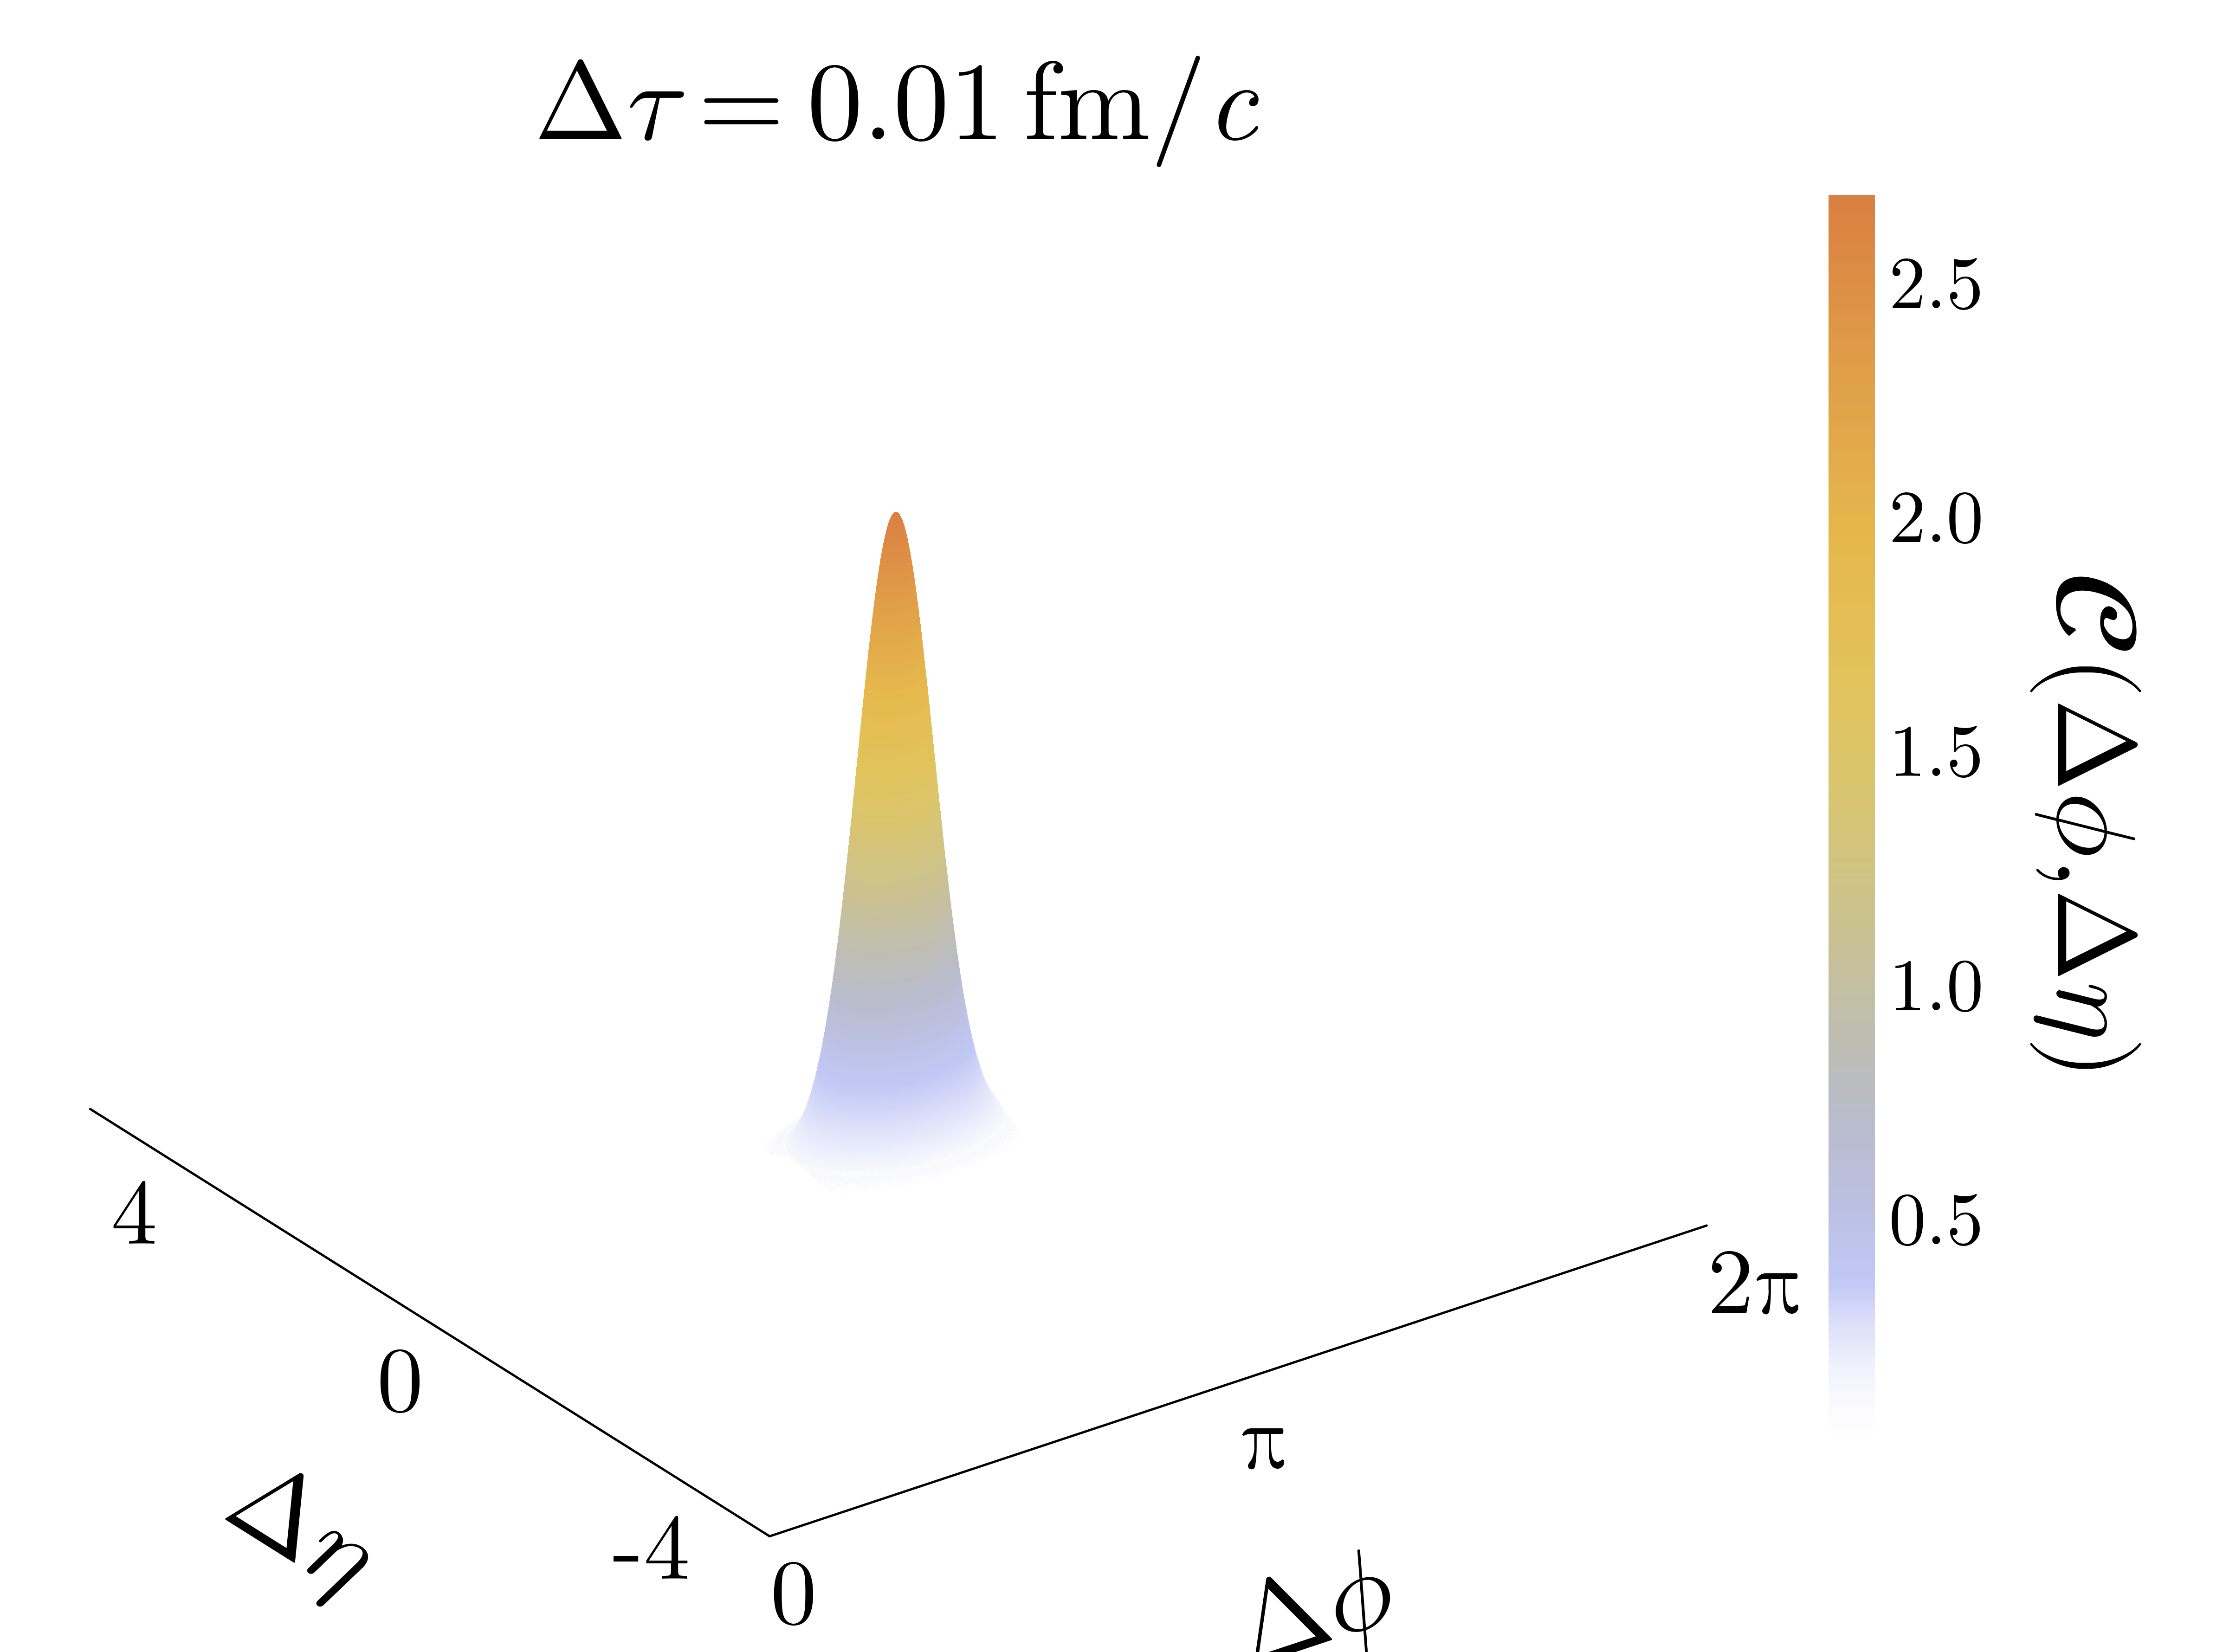
\includegraphics[width=0.5\columnwidth]
                    {images/paper_Cdetadphi_3D_toy_charm_pT_1_tau_0.01_v2.png}\hfill
                    % \includegraphics[width=0.31\columnwidth]
                    % {images/paper_Cdetadphi_3D_toy_charm_pT_1_tau_0.1_v2.png}\quad
                    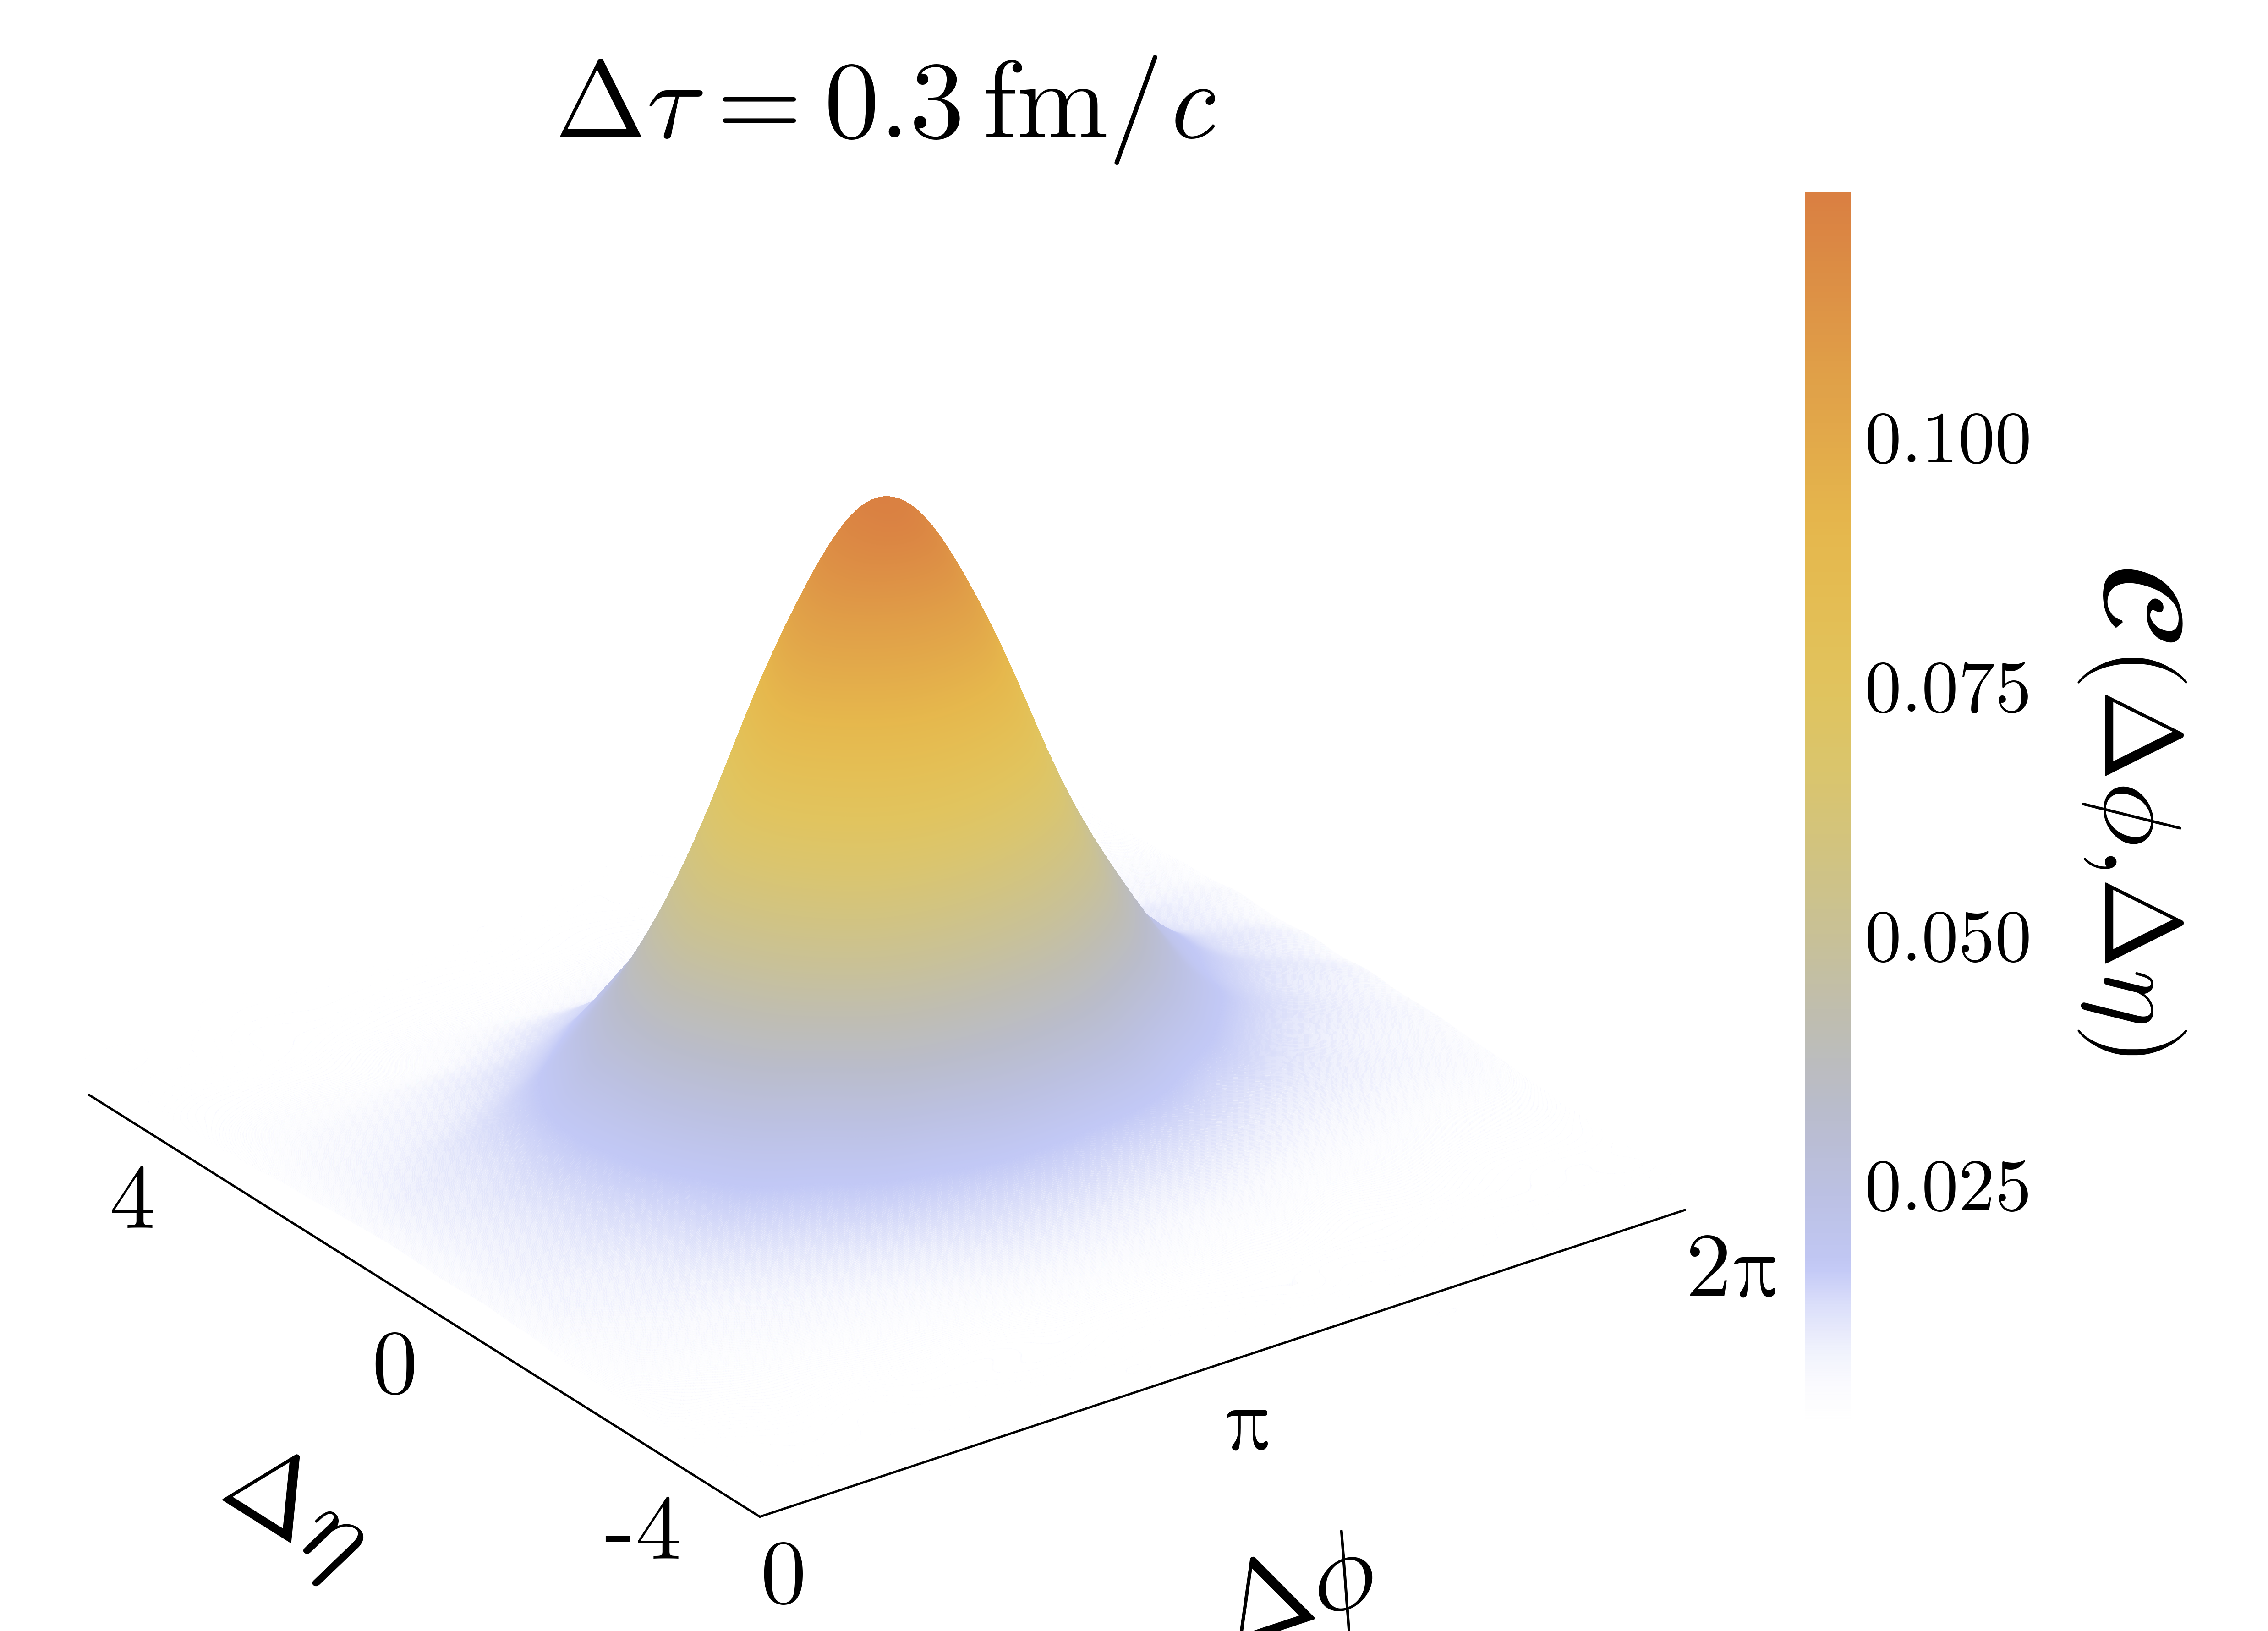
\includegraphics[width=0.5\columnwidth]
                    {images/paper_Cdetadphi_3D_toy_charm_pT_1_tau_0.3_v2.png}
                \end{figure}
            \end{center}
            \column{.02\textwidth}
            \column{.36\textwidth}
            \begin{center}
                \begin{custombox2}{\normalsize Azimuthal decorrelation}{palgold}
                    \small
                    \begin{varwidth}{0.98\textwidth}
                    \begin{itemize}\itemsep0em 
                        \itemsep0em
                        \footnotesize
                        \setbeamertemplate{itemize item}{\raisebox{0.2em}{\scalebox{0.7}{${\color{palgold}\blacktriangleright}$}}} 
                        \item {\bfseries\color{palgold}$\boldsymbol{D\overline{D}}$ angular correlations}
                        \item Decorrelation width $\sigma_{\Delta\phi}(\Delta\tau)$
                    \end{itemize}
                    \end{varwidth}
                \end{custombox2}

                \vspace{-10pt}
                \begin{figure}
                    \centering
                    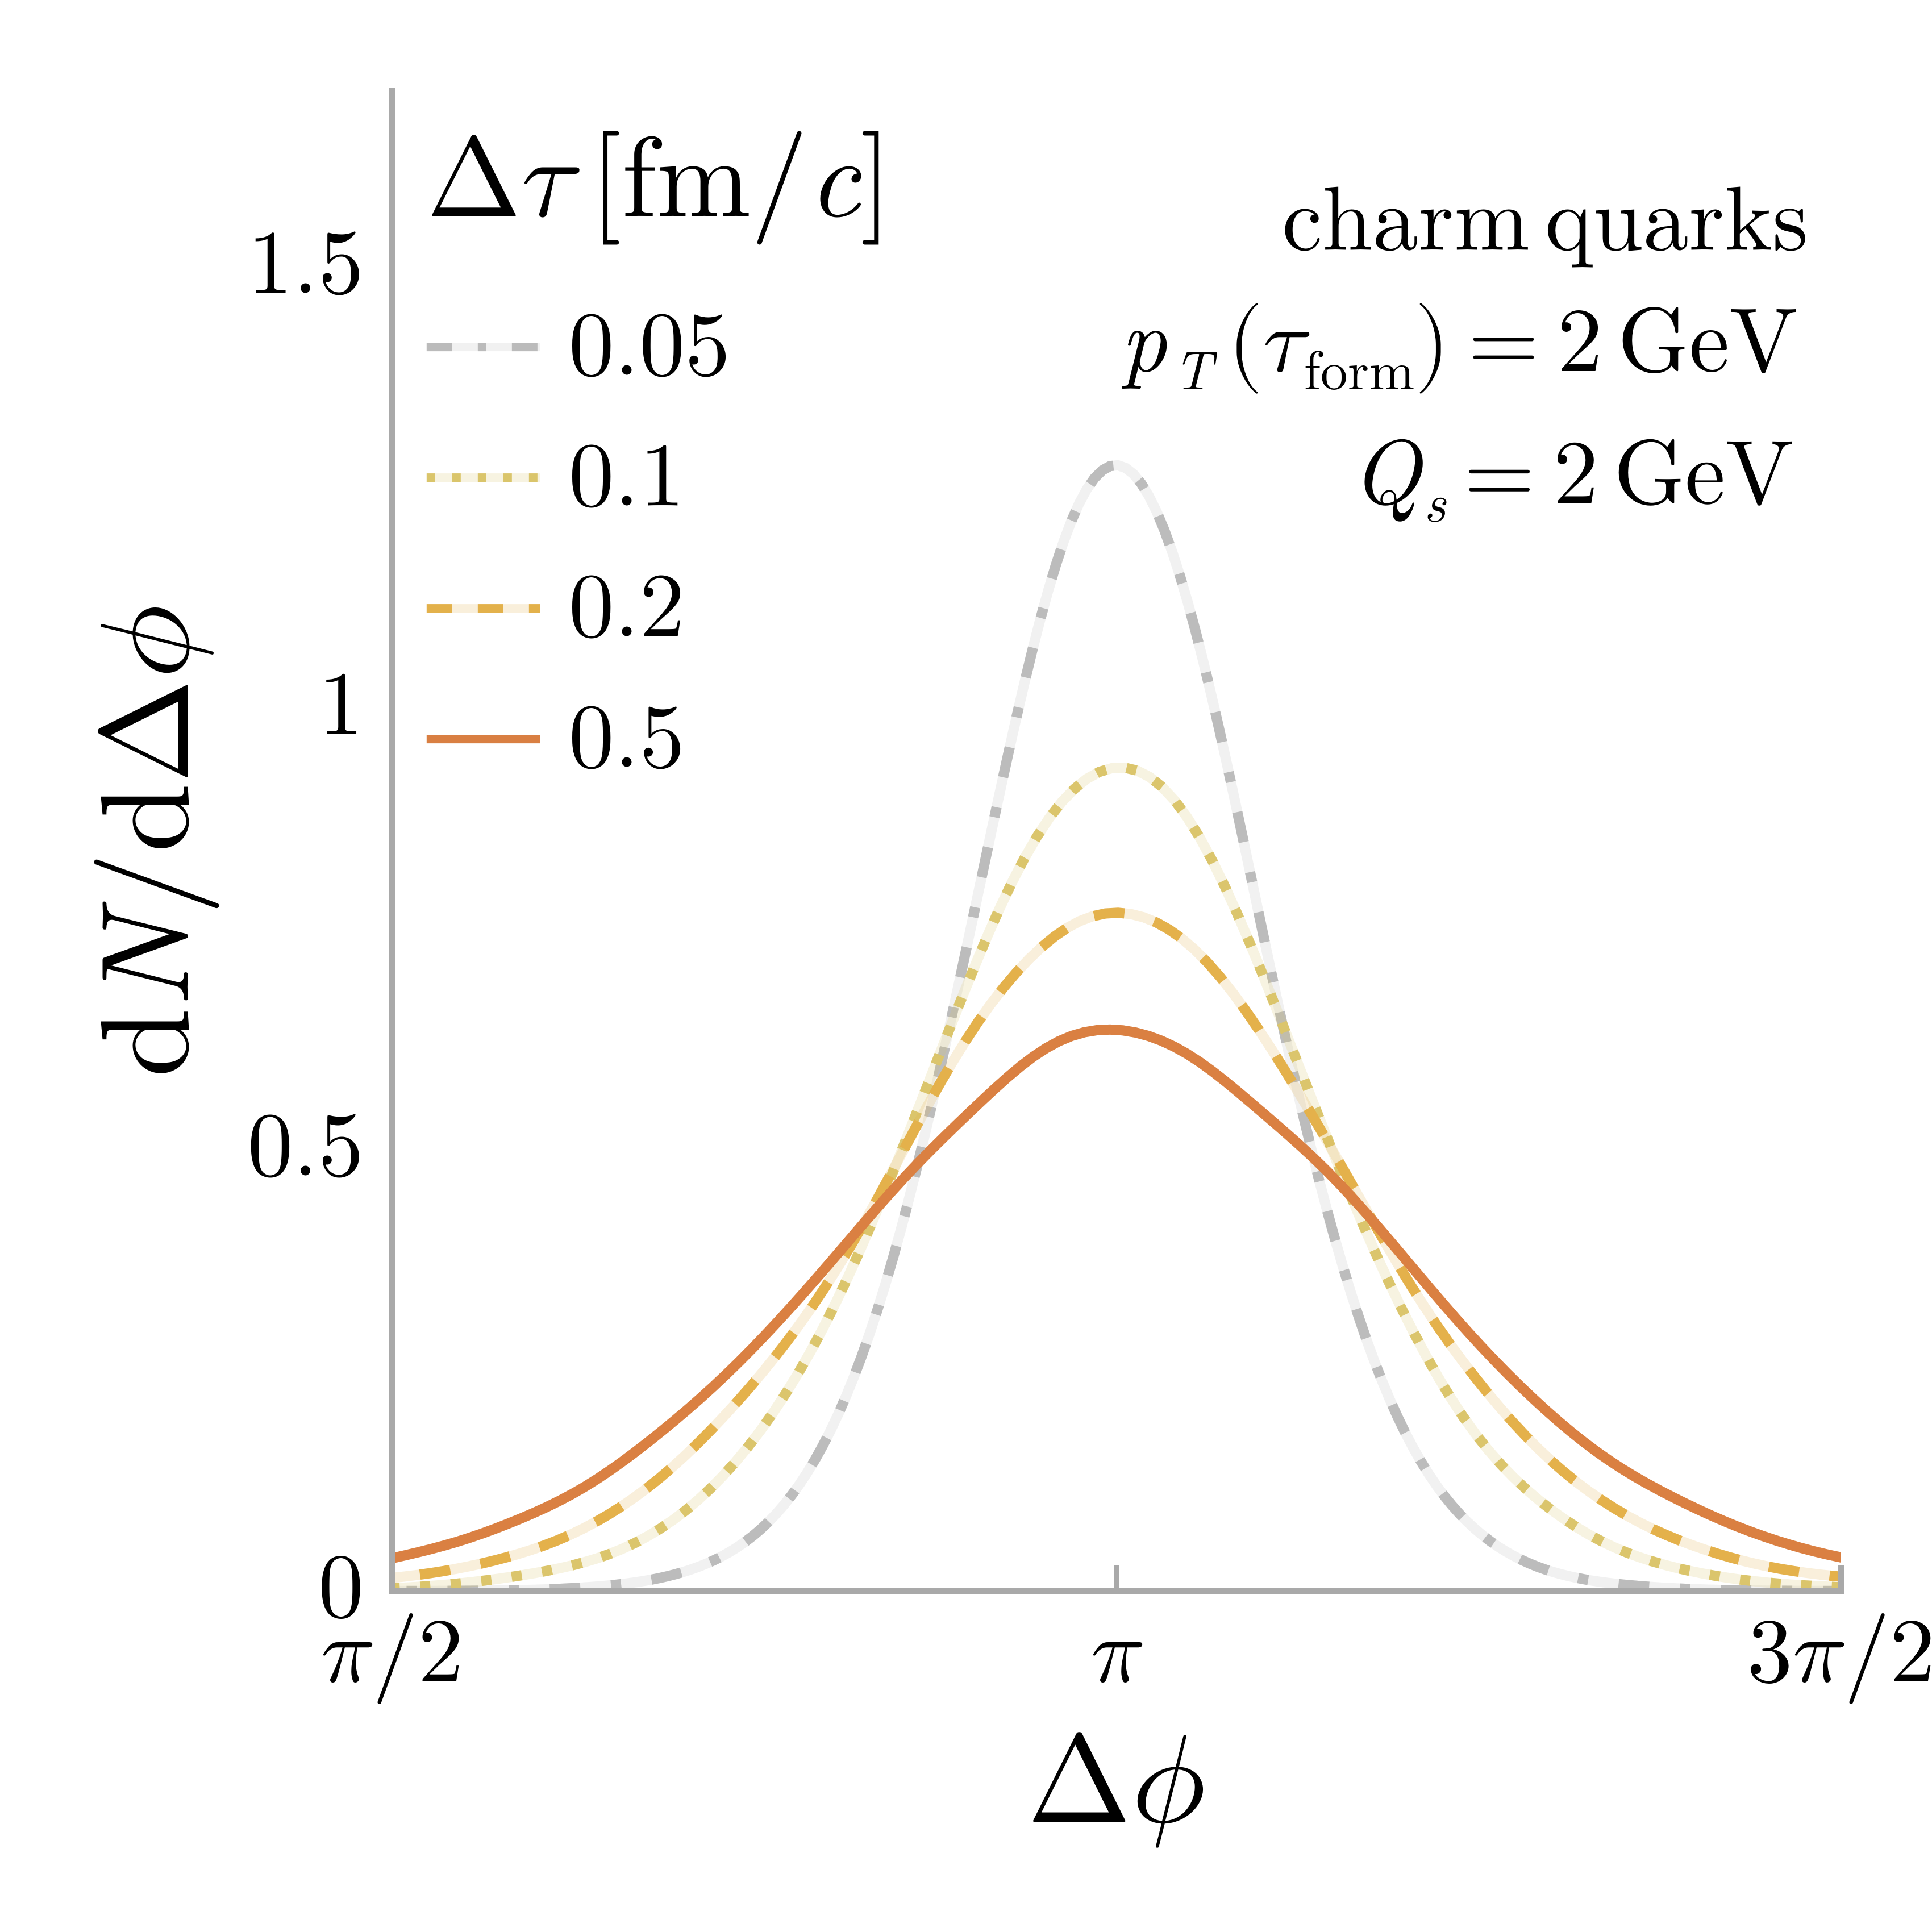
\includegraphics[width=0.8\columnwidth]{images/final_dNdphi_tau_dep_charm_v2.png}
                \end{figure}
            \end{center}
            \column{.02\textwidth}
        \end{columns}    

    \end{center}
    \vspace{-10pt}
    \blfootnote{\scriptsize ALICE 3 Letter of Intent \href{https://arxiv.org/abs/2211.02491}{{\color{palgold}\texttt{[2211.02491]$^\text{\tiny\faExternalLink}$}}}}
    
\end{frame}

%%%%%%%%%%%%%%%%%%%%%%%%%%%%%%%%%%%%%%%%%
%%%%%%%%%%%%%%%%% SLIDE %%%%%%%%%%%%%%%%%
%%%%%%%%%%%%%%%%%%%%%%%%%%%%%%%%%%%%%%%%%

\begin{frame}[noframenumbering]
    \frametitle{Decorrelation of $Q\overline{Q}$ pairs}
    % \framesubtitle{Quantifying the decorrelation in glasma}
    {\transparent{0.1}
    % \vspace{-5pt}
    \begin{center}
        \begin{columns}[onlytextwidth,t]
            \column{.02\textwidth}
           \column{.58\textwidth}
           \begin{center}
                \begin{custombox2transp}{\normalsize\transparent{0.1} Decorrelation in glasma}{lightgray}
                    \small
                    \begin{varwidth}{1.02\textwidth}
                    \begin{itemize}\itemsep0em 
                        \itemsep0em
                        \footnotesize
                        \setbeamertemplate{itemize item}{\raisebox{0.2em}{\scalebox{0.7}{${\color{lightgray}\blacktriangleright}$}}} 
                        \item \transparent{0.1}Two-particle correlations $\boldsymbol{\mathcal{C}(\Delta\phi, \Delta\eta)}$ at $\boldsymbol{\Delta\tau}=\tau-\tau_\mathrm{form}$
                        \item \transparent{0.1}Initial peak $\delta(\Delta\phi-\pi)\delta(\Delta\eta)$ gets broadened by glasma
                    \end{itemize}
                    \end{varwidth}
                \end{custombox2transp}
                % \begin{itemize}\itemsep0em 
                %     \itemsep0em
                %     \footnotesize\color{lightgray}
                %     \setbeamertemplate{itemize item}{\raisebox{0.2em}{\scalebox{0.7}{${\color{lightgray}\blacktriangleright}$}}} 
                %     \item Two-particle correlations extracted as\\
                %     $\mathcal{C}(\Delta\phi, \Delta\eta)=\dfrac{1}{N_\mathrm{pairs}}\dfrac{\mathrm{d}^2N}{\mathrm{d}\Delta\phi\mathrm{d}\Delta\eta}$
                % \end{itemize}

                \begin{figure}
                    \centering
                    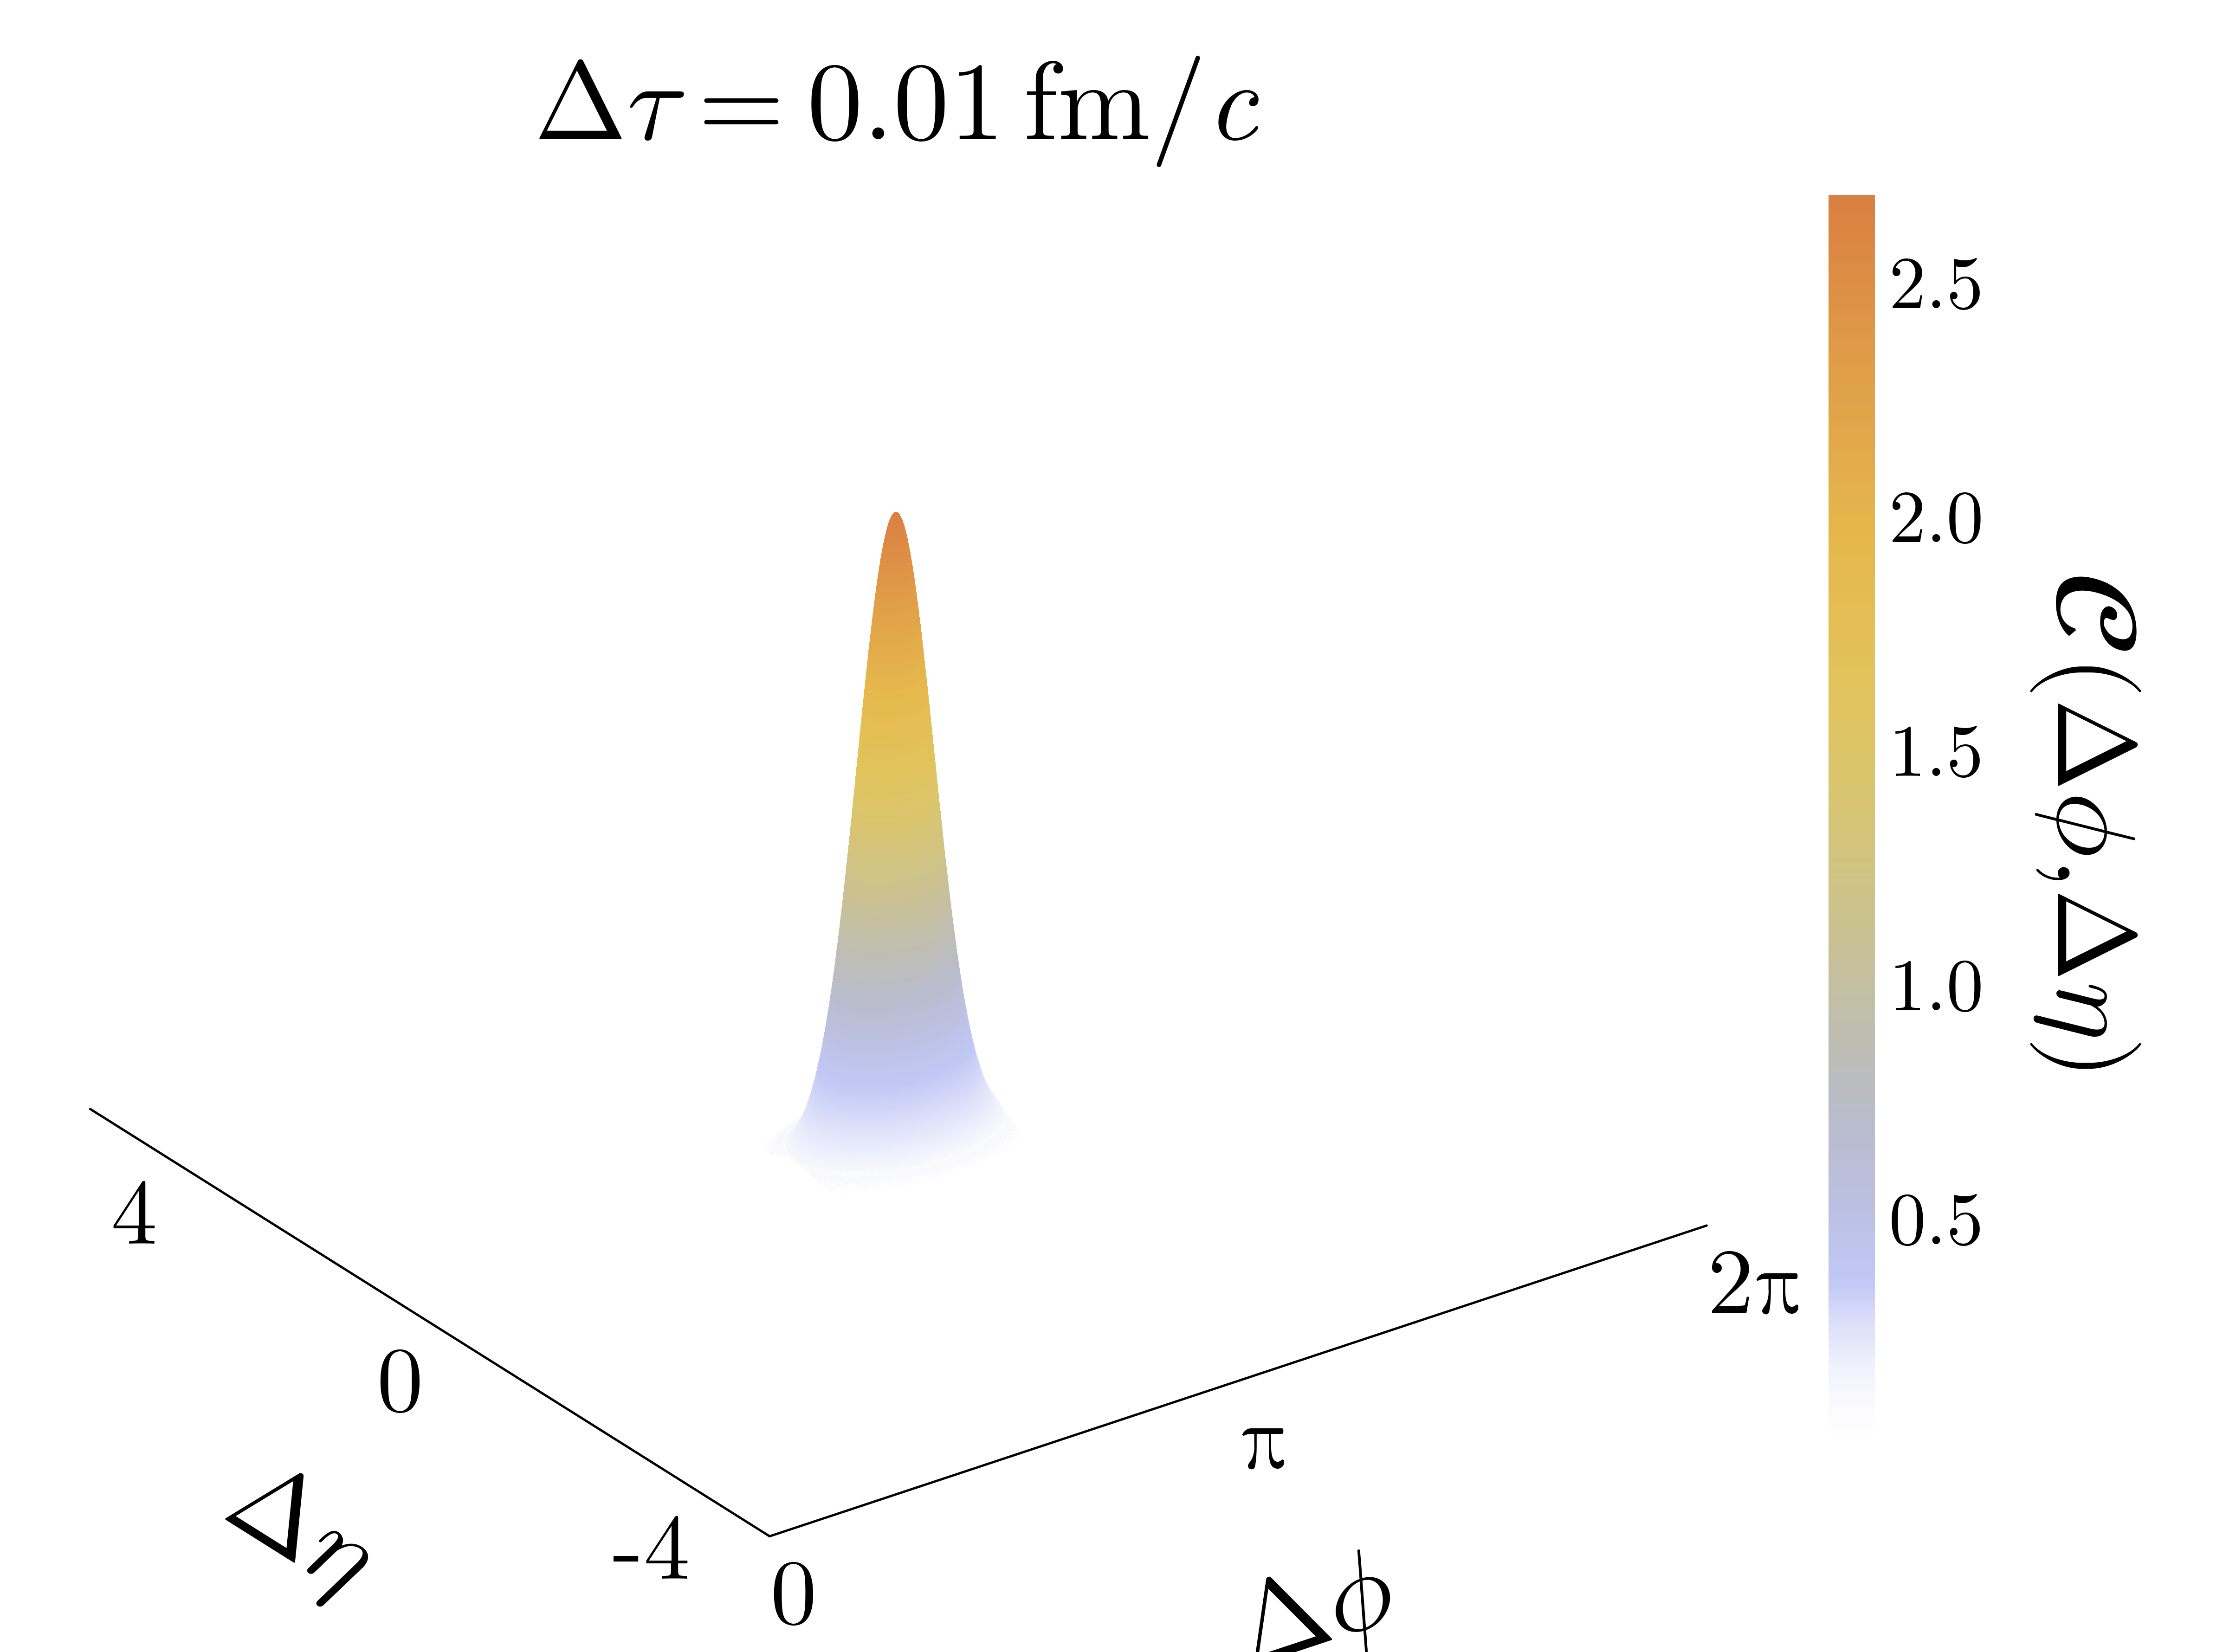
\includegraphics[width=0.5\columnwidth]
                    {images/paper_Cdetadphi_3D_toy_charm_pT_1_tau_0.01_v2.png}\hfill
                    % \includegraphics[width=0.31\columnwidth]
                    % {images/paper_Cdetadphi_3D_toy_charm_pT_1_tau_0.1_v2.png}\quad
                    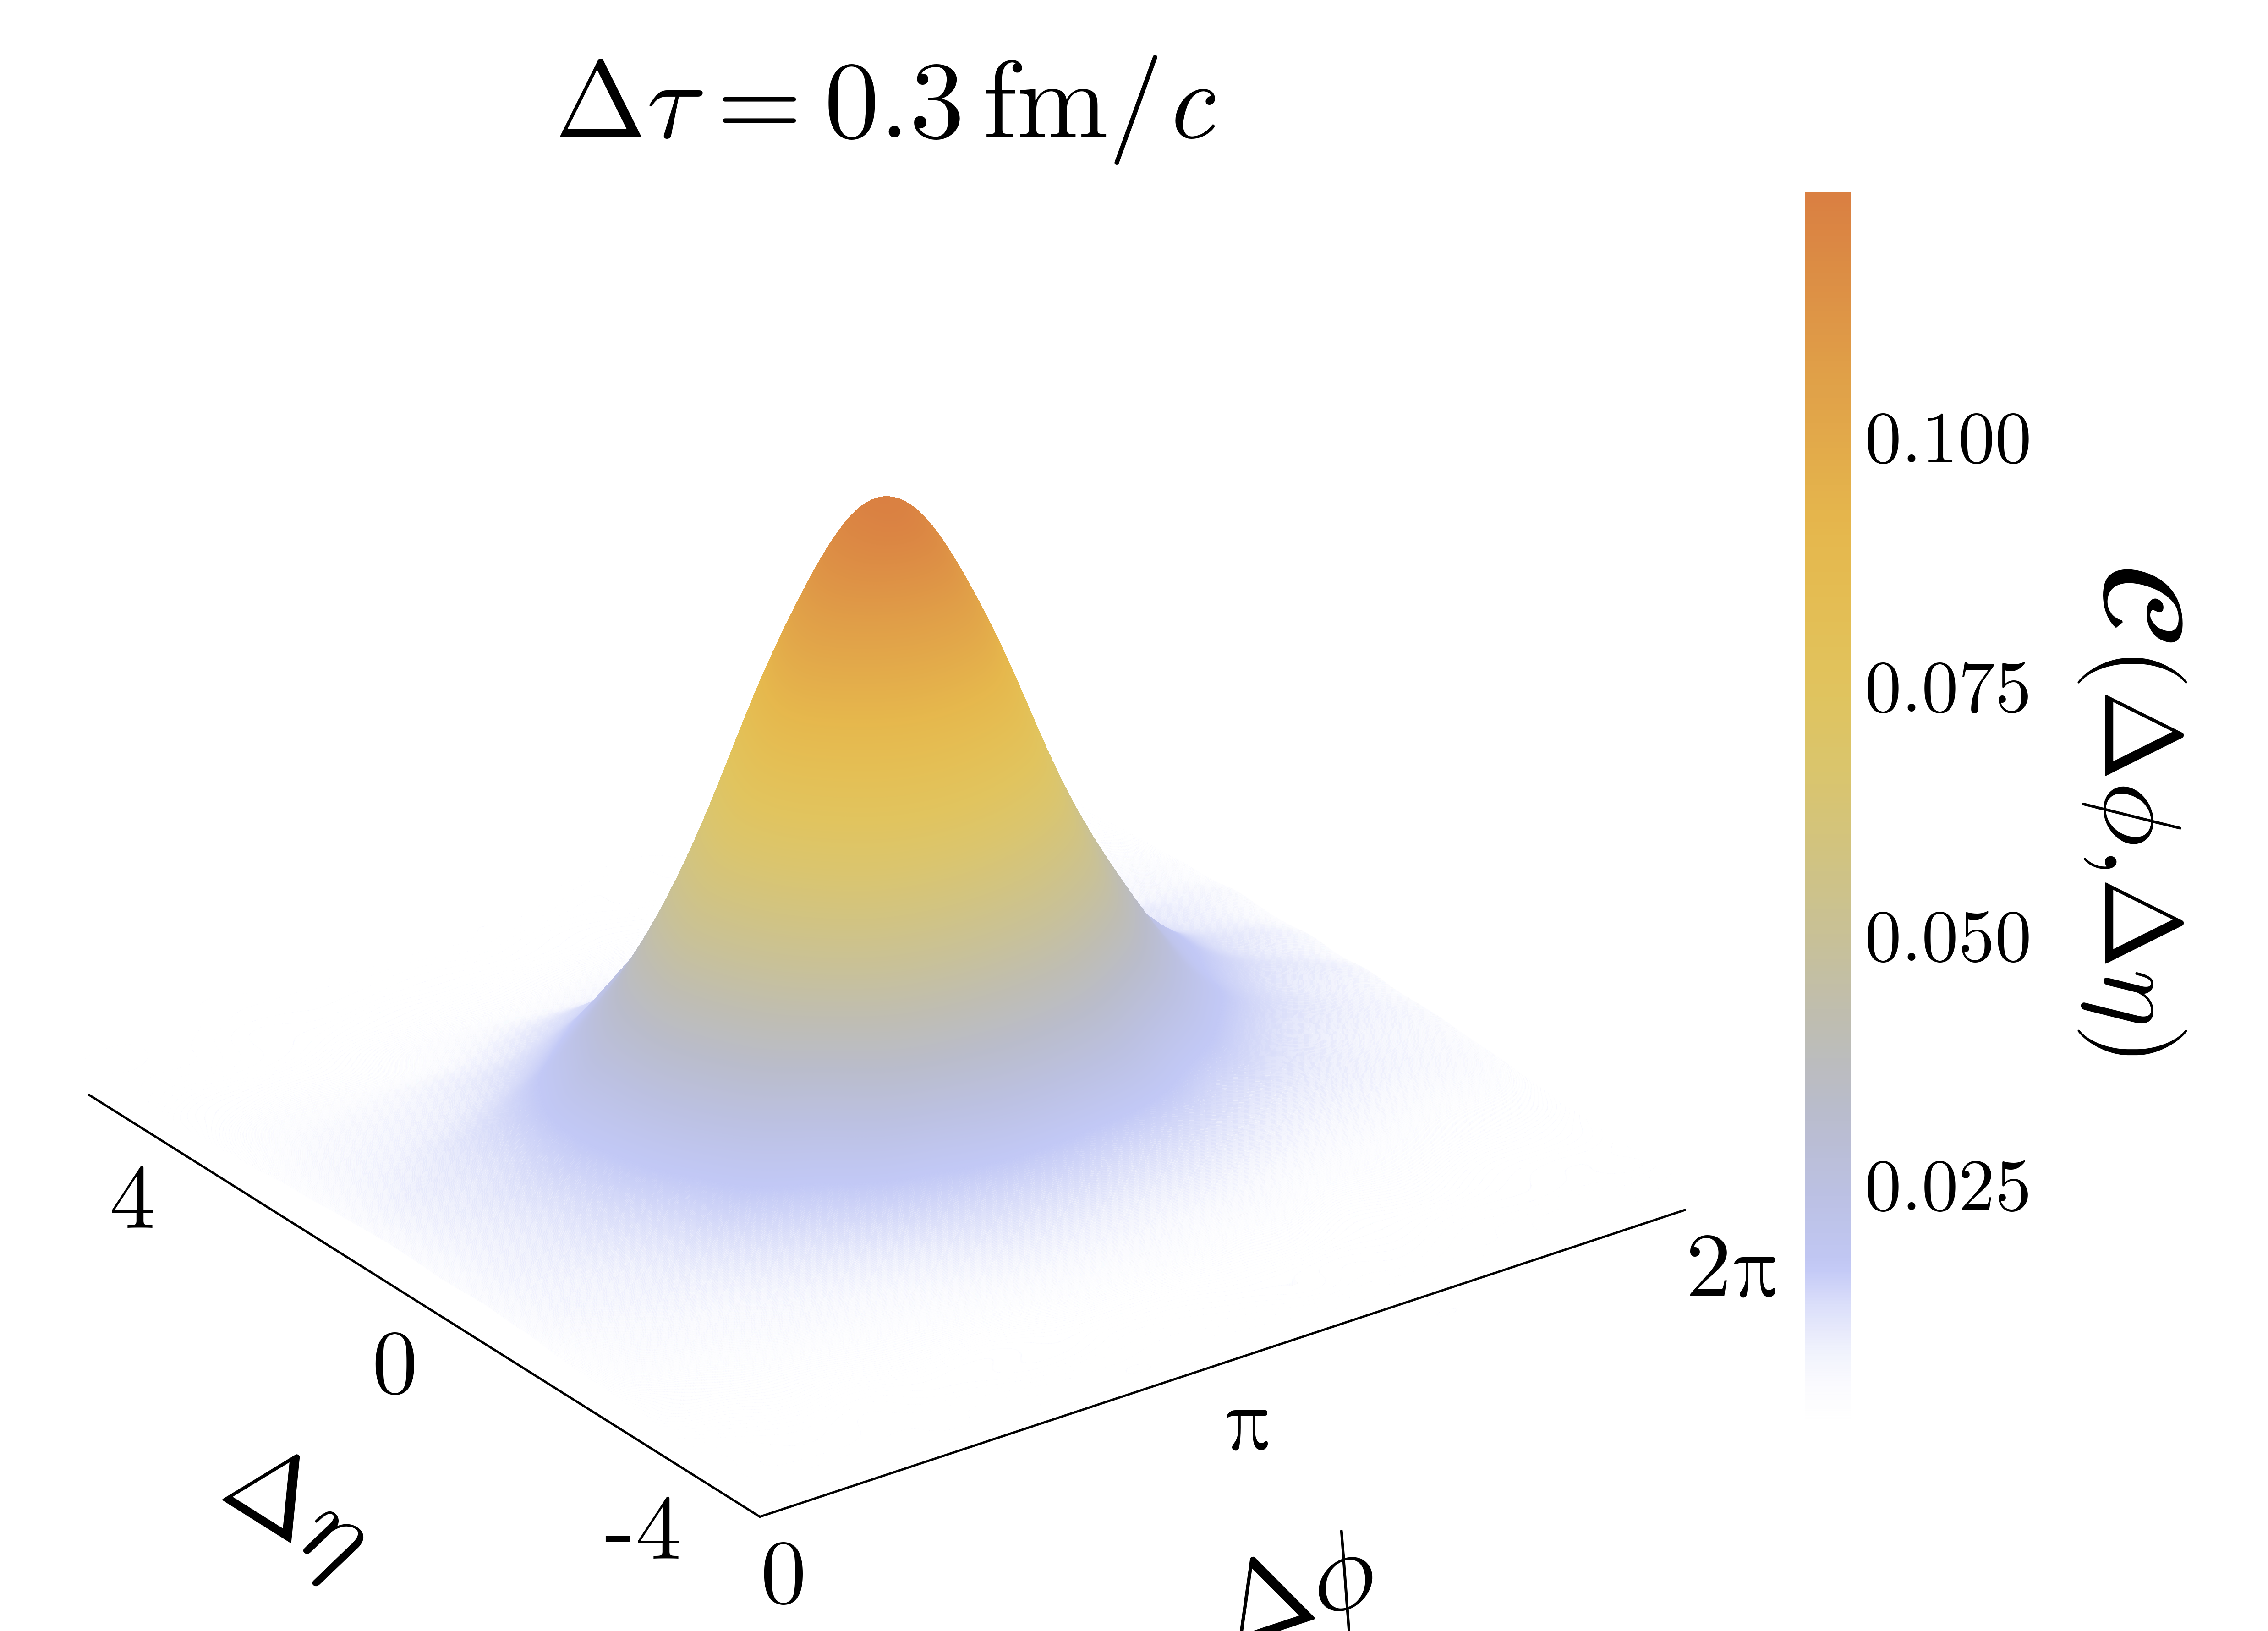
\includegraphics[width=0.5\columnwidth]
                    {images/paper_Cdetadphi_3D_toy_charm_pT_1_tau_0.3_v2.png}
                \end{figure}
            \end{center}
            \column{.02\textwidth}
            \column{.36\textwidth}
            \begin{center}
                \begin{custombox2transp}{\normalsize \transparent{0.1}Azimuthal decorrelation}{palgold}
                    \small
                    \begin{varwidth}{0.98\textwidth}
                    \begin{itemize}\itemsep0em 
                        \itemsep0em
                        \footnotesize
                        \setbeamertemplate{itemize item}{\raisebox{0.2em}{\scalebox{0.7}{${\color{palgold}\blacktriangleright}$}}} 
                        \item \transparent{0.1}{\bfseries\color{palgold}$\boldsymbol{D\overline{D}}$ angular correlations}
                        \item \transparent{0.1}Decorrelation width $\sigma_{\Delta\phi}(\Delta\tau)$
                    \end{itemize}
                    \end{varwidth}
                \end{custombox2transp}

                \vspace{-10pt}
                \begin{figure}
                    \centering
                    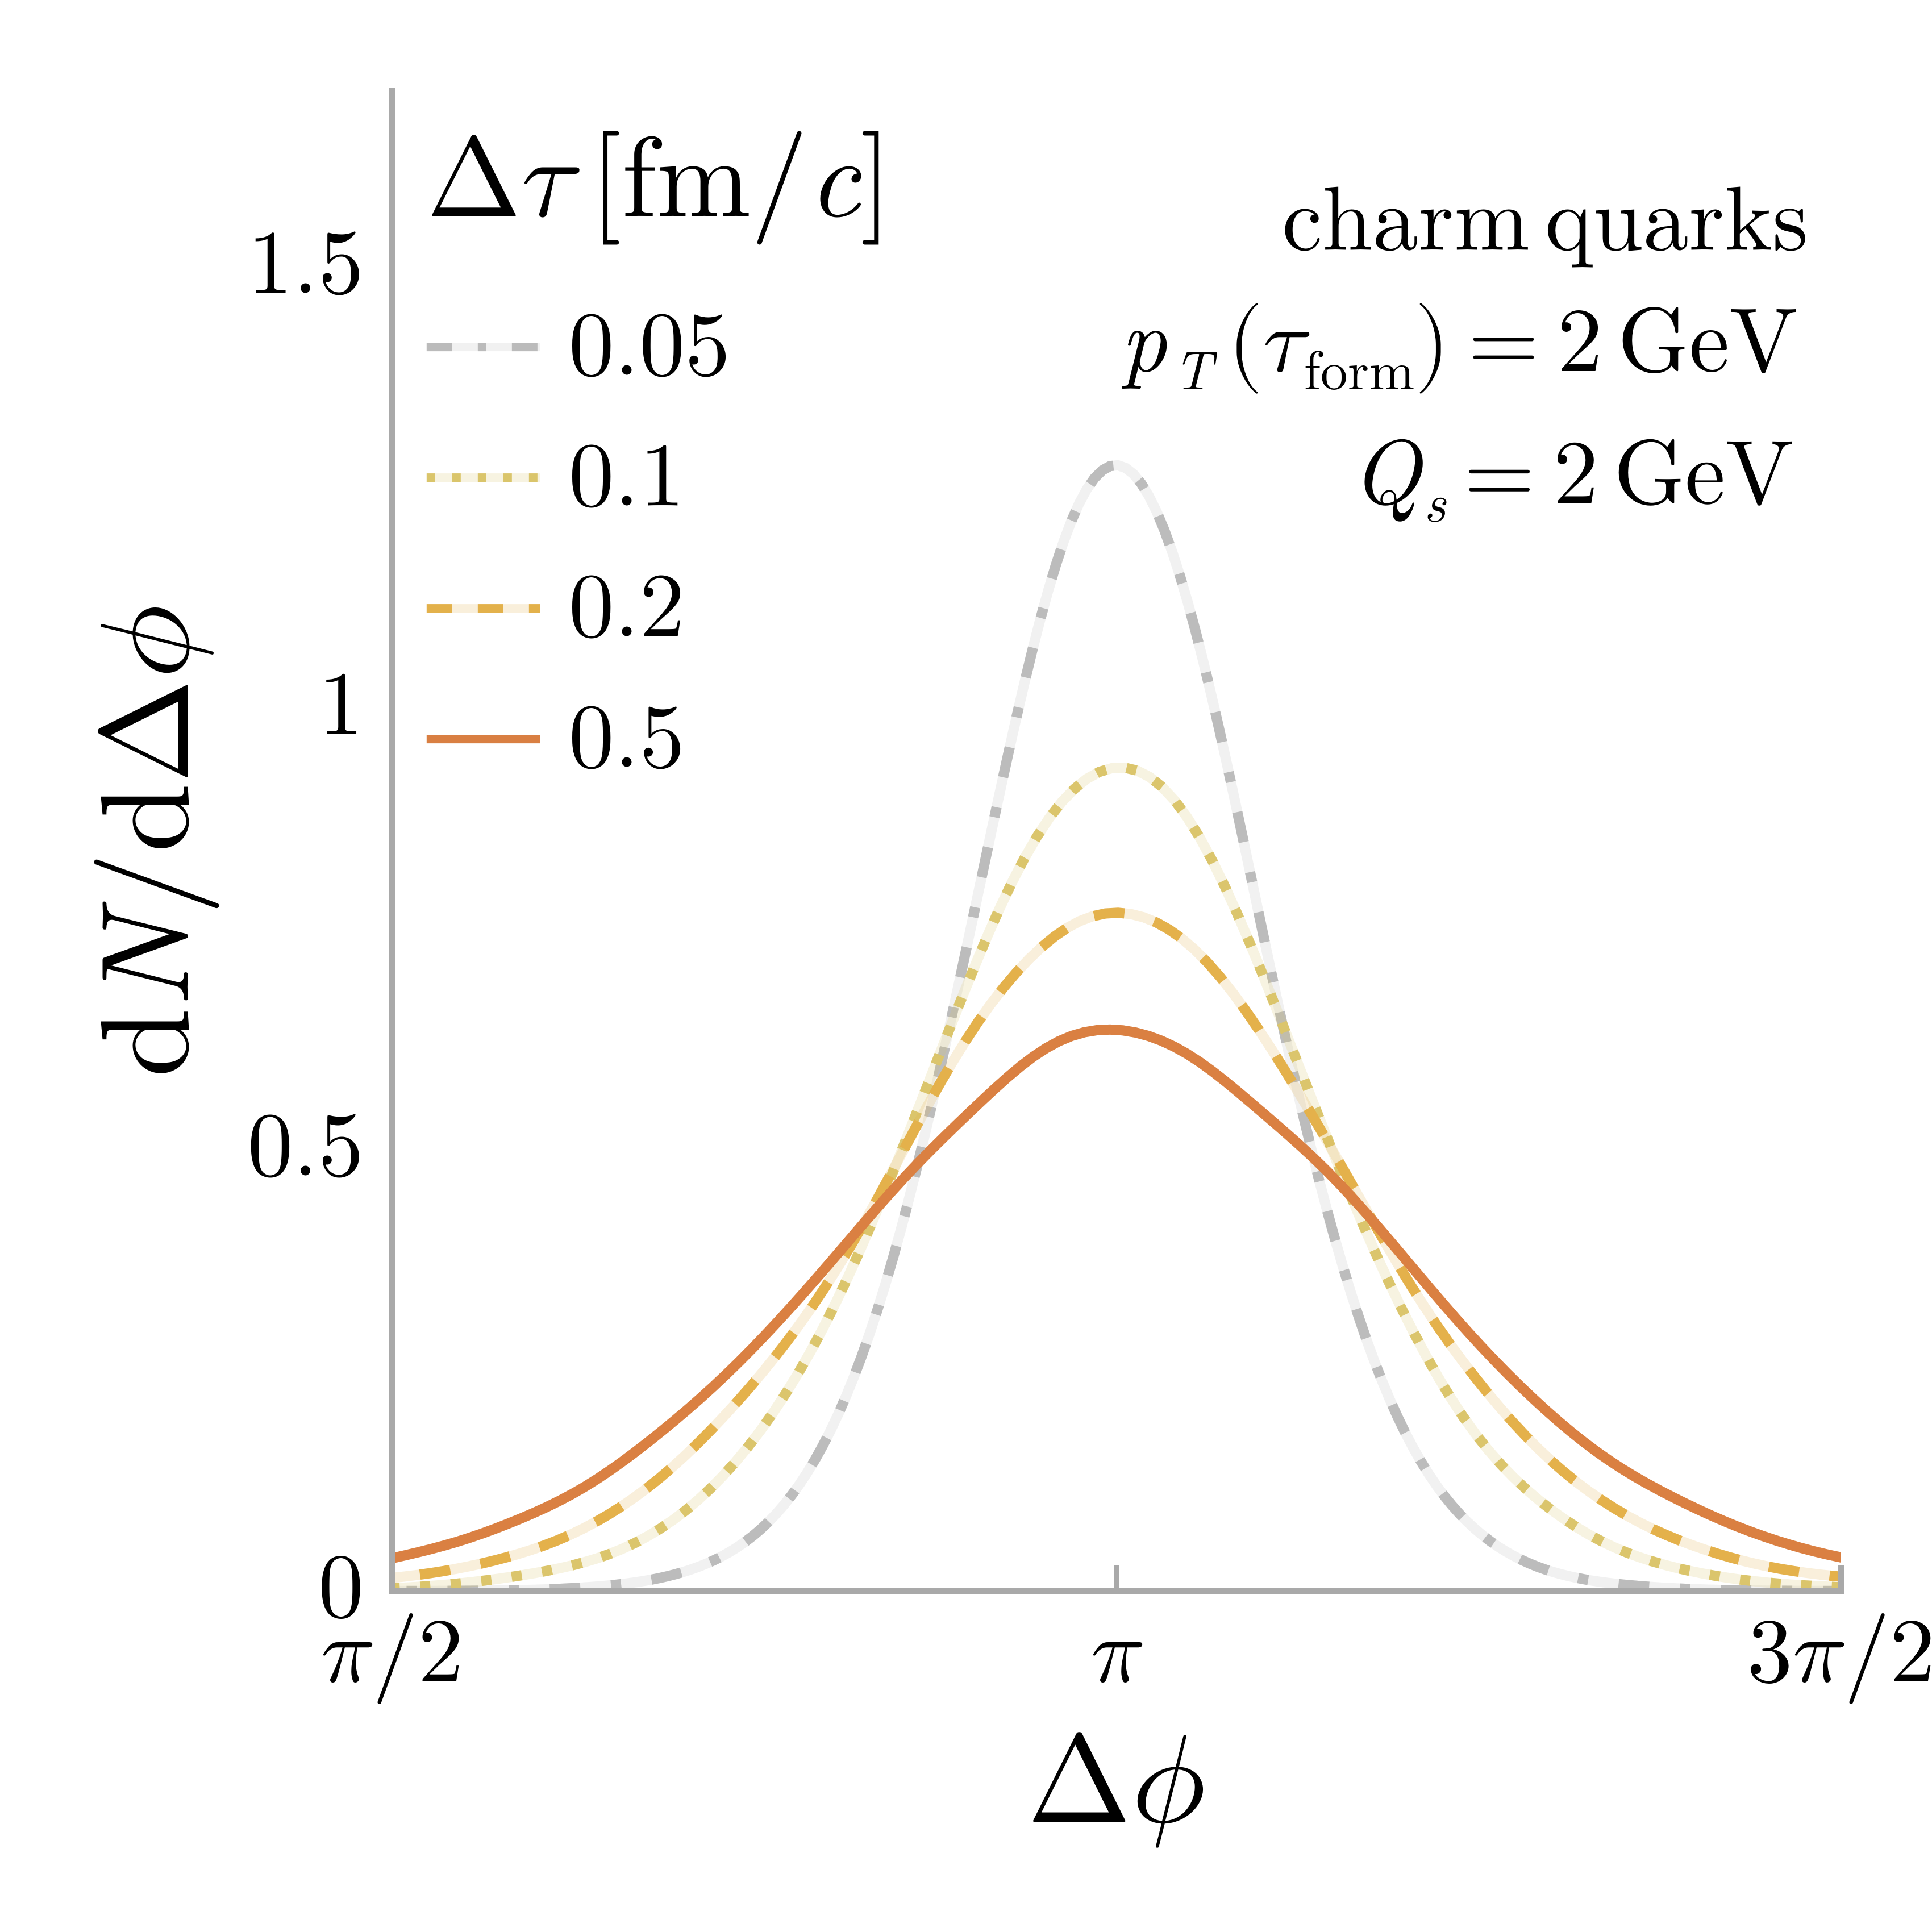
\includegraphics[width=0.8\columnwidth]{images/final_dNdphi_tau_dep_charm_v2.png}
                \end{figure}
            \end{center}
            \column{.02\textwidth}
        \end{columns}    

    \end{center}
    % \vspace{-10pt}
    % \blfootnote{\scriptsize \transparent{0.1}ALICE 3 Letter of Intent \href{https://arxiv.org/abs/2211.02491}{{\color{palgold}\texttt{[2211.02491]$^\text{\tiny\faExternalLink}$}}}}
    }

    \begin{center}
        \vspace{-10pt}
        \begin{tikzpicture}[remember picture,overlay]
            \node[align=center] at (0,4) {
                \large \textit{Candidate observable}\\[5pt]
                \huge Heavy quarks $\mathcal{C}(\Delta\phi)$\\[15pt]
                \Large Glasma causes {\color{palgold}azimuthal decorrelation}\\[7pt]
                \Large {\color{palgold}Large effect} compared to LO back-to-back 
            };
        \end{tikzpicture} 
    \end{center}
\end{frame}


%%%%%%%%%%%%%%%%%%%%%%%%%%%%%%%%%%%%%%%%%
%%%%%%%%%%%%%%%%% SLIDE %%%%%%%%%%%%%%%%%
%%%%%%%%%%%%%%%%%%%%%%%%%%%%%%%%%%%%%%%%%

\begin{frame}
    \frametitle{Where does the correlation go?}
    % \framesubtitle{Available models}
    \vspace{-15pt}
    \begin{center}
        \begin{columns}[onlytextwidth,t]
            % \column{.01\textwidth}
           \column{.47\textwidth}
           \begin{center}
                \begin{custombox2}{\normalsize Glasma+Wong approach}{palgold}
                    \small
                    \begin{varwidth}{0.93\textwidth}
                    \begin{itemize}\itemsep0em 
                        \itemsep0em
                        \footnotesize
                        \setbeamertemplate{itemize item}{\raisebox{0.2em}{\scalebox{0.7}{${\color{palgold}\blacktriangleright}$}}} 
                        \item Decorrelation due to initial {\bfseries\color{palgold}glasma field}
                        \item Small $p_T$ pairs {\bfseries\color{palgold}decorrelate immediately} 
                    \end{itemize}
                    \end{varwidth}
                \end{custombox2}
            \end{center}
            \vspace{-15pt}
           \begin{figure}
                \centering
                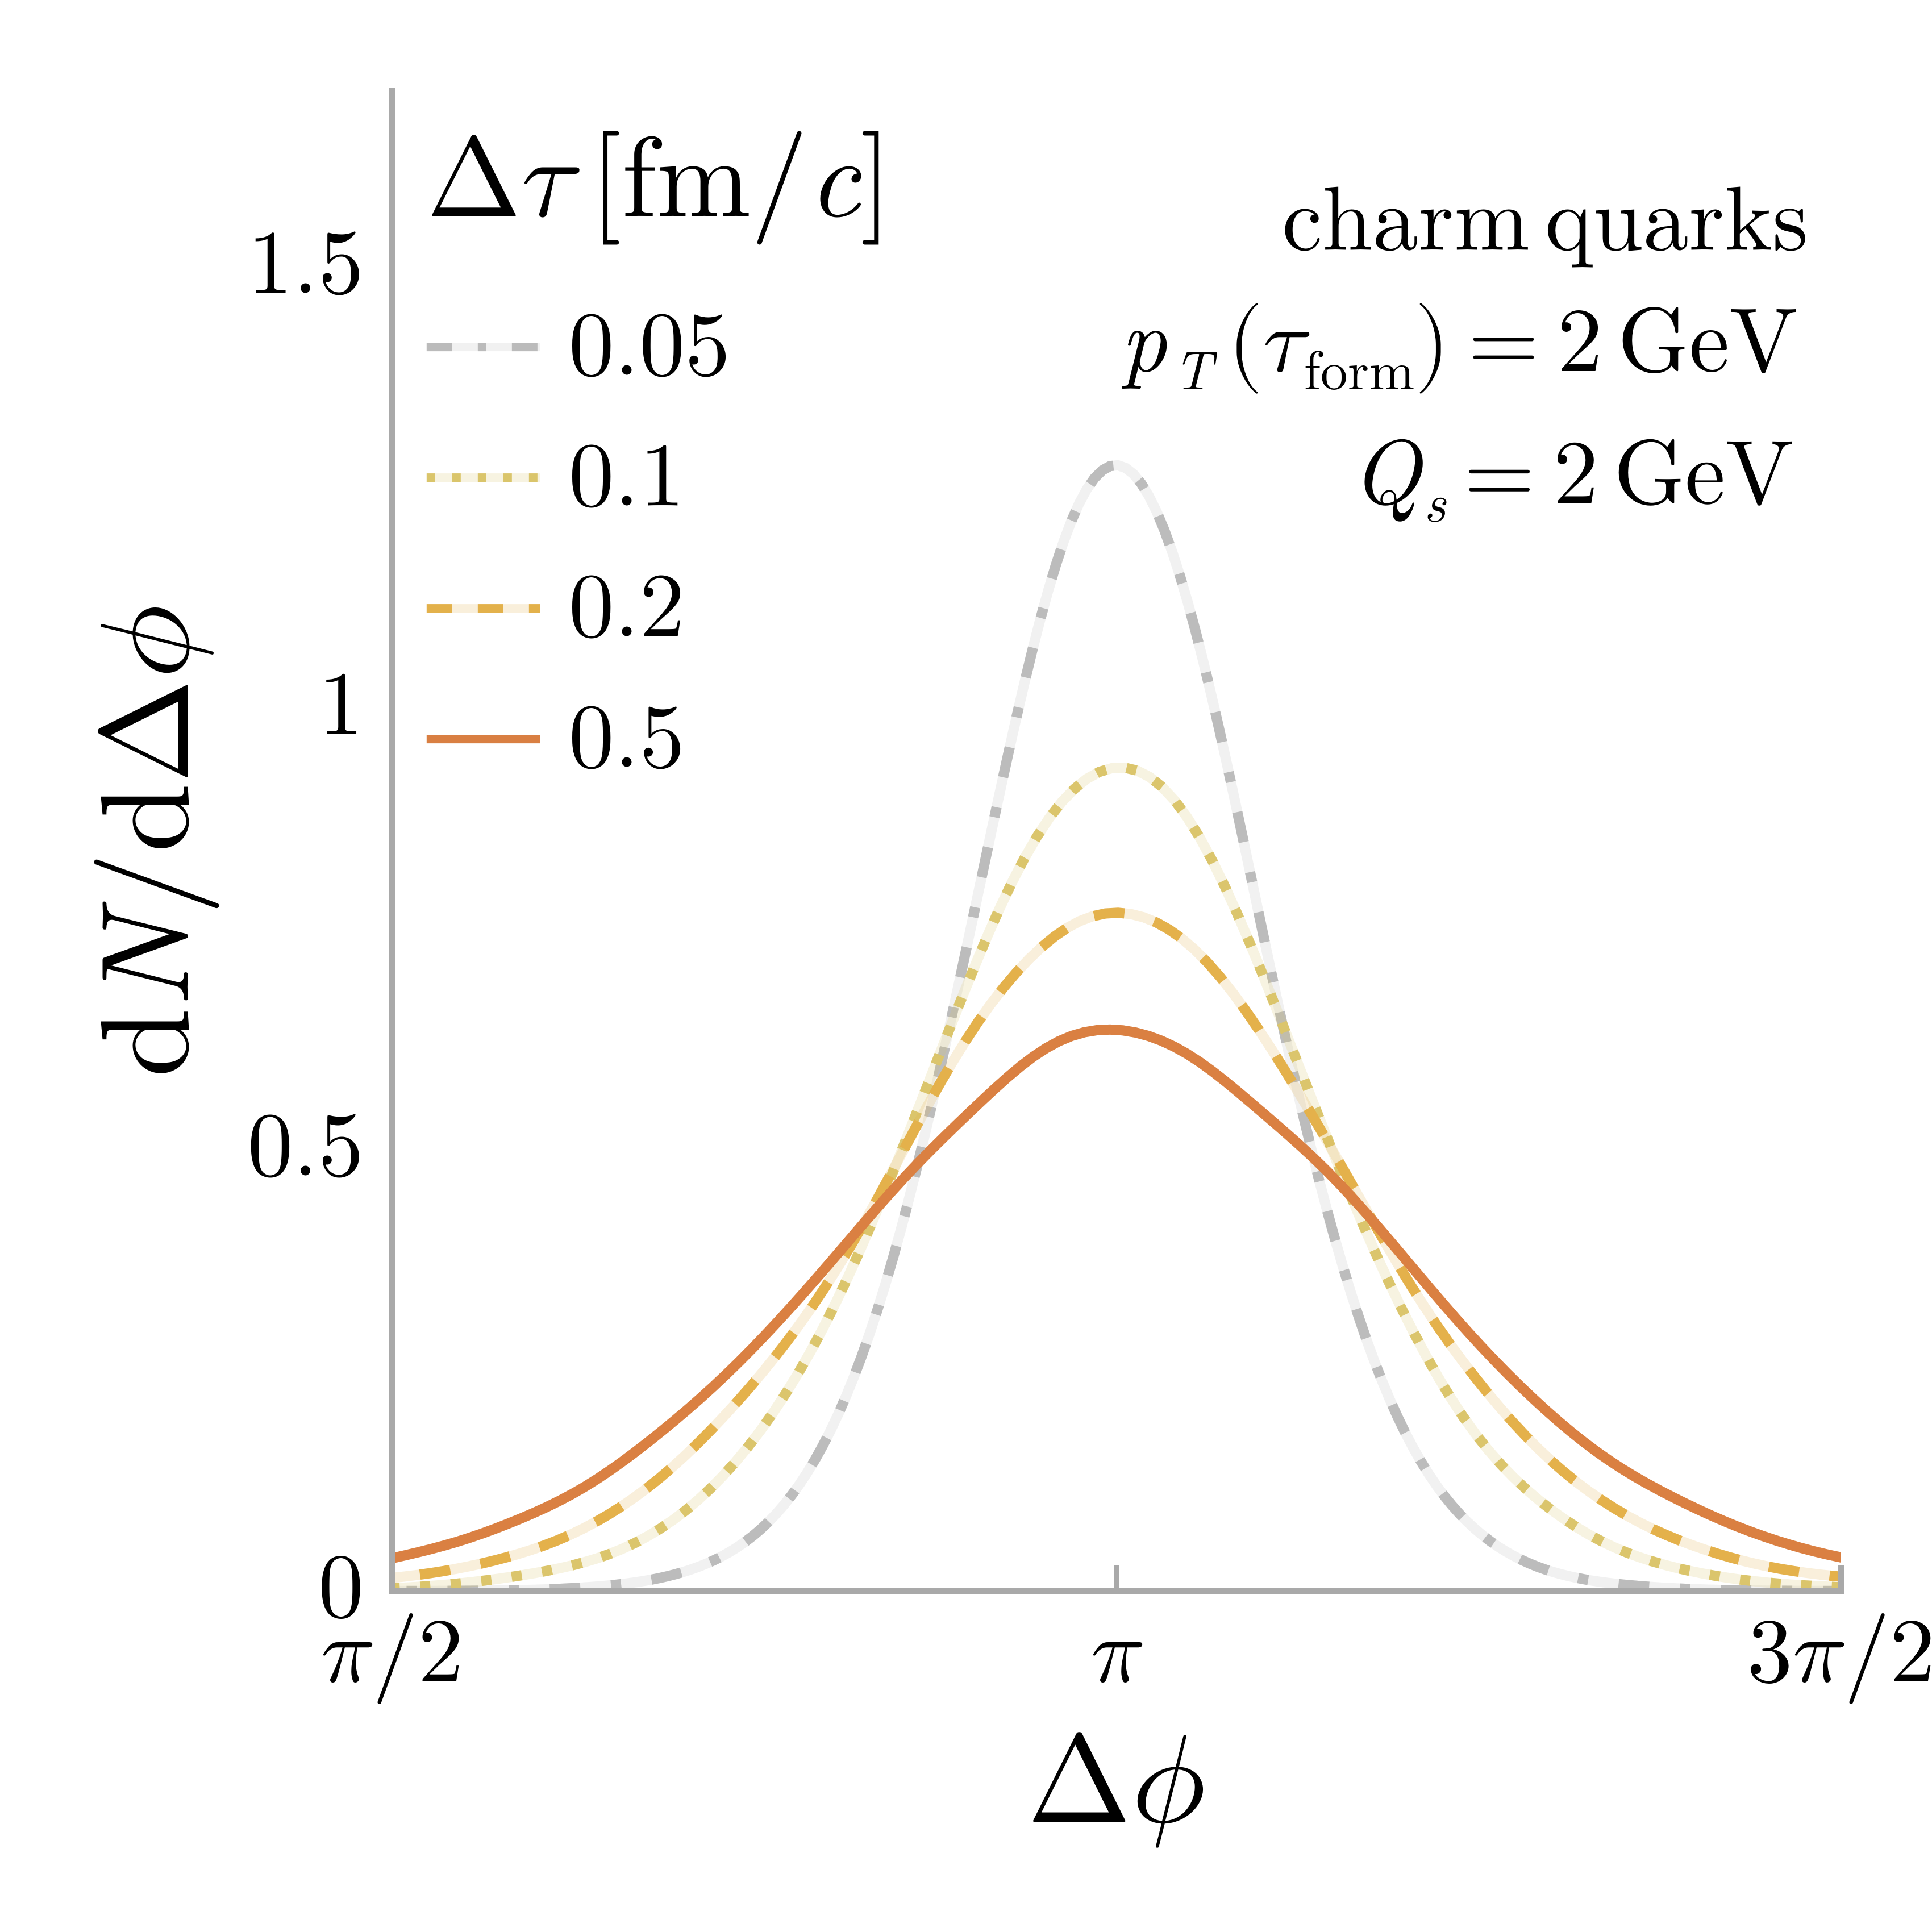
\includegraphics[width=0.7\columnwidth]{images/final_dNdphi_tau_dep_charm_v2.png}
            \end{figure}
            \column{.01\textwidth}
            \column{.49\textwidth}
            \begin{center}
                \begin{custombox2}{\normalsize MC@sHQ+EPOS model}{Orange}
                    \small
                    \begin{varwidth}{1.06\textwidth}
                    \begin{itemize}\itemsep0em 
                        \itemsep0em
                        \footnotesize
                        \setbeamertemplate{itemize item}{\raisebox{0.2em}{\scalebox{0.7}{${\color{Orange}\blacktriangleright}$}}} 
                        \item Decorrelation due to {\bfseries\color{Orange}transport in medium}
                        \item Collisional + radiative energy loss effects
                        \item Small $p_T$ pairs {\bfseries\color{Orange}decorrelate throughout evolution}
                    \end{itemize}
                    \end{varwidth}
                \end{custombox2}
            \end{center}
            \vspace{-10pt}
            % \vspace{-7pt}
            \begin{figure}
                \centering
                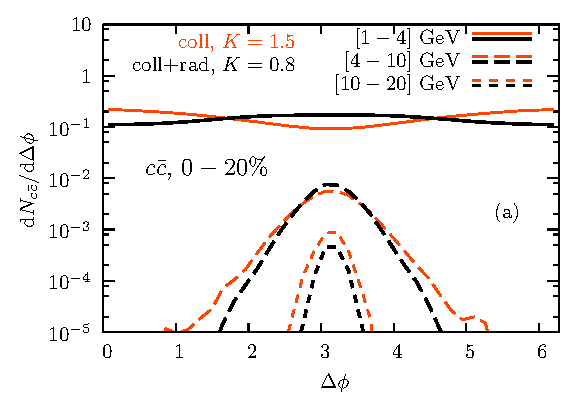
\includegraphics[width=0.83\columnwidth]{images/deltaphi_cccor_centrala.eps}
            \end{figure}
            \column{.02\textwidth}
        \end{columns}    
    \end{center}
    \vspace{-15pt}
    \blfootnote{\scriptsize Nahrgang, Aichelin, Gossiaux, Werner \href{https://arxiv.org/abs/1305.3823}{{\color{Orange}\texttt{[1305.3823]$^\text{\tiny\faExternalLink}$}}}}
\end{frame}

%%%%%%%%%%%%%%%%%%%%%%%%%%%%%%%%%%%%%%%%%
%%%%%%%%%%%%%%%%% SLIDE %%%%%%%%%%%%%%%%%
%%%%%%%%%%%%%%%%%%%%%%%%%%%%%%%%%%%%%%%%%

\begin{frame}[noframenumbering]
    \frametitle{Where does the correlation go?}
    % \framesubtitle{Available models}
    {\transparent{0.1}\vspace{-15pt}
    \begin{center}
        \begin{columns}[onlytextwidth,t]
            % \column{.01\textwidth}
           \column{.47\textwidth}
           \begin{center}
                \begin{custombox2transp}{\normalsize \transparent{0.1}Glasma+Wong approach}{palgold}
                    \small
                    \begin{varwidth}{0.93\textwidth}
                    \begin{itemize}\itemsep0em 
                        \itemsep0em
                        \footnotesize
                        \setbeamertemplate{itemize item}{\raisebox{0.2em}{\scalebox{0.7}{${\color{palgold}\blacktriangleright}$}}} 
                        \item \transparent{0.1}Decorrelation due to initial {\bfseries\color{palgold}glasma field}
                        \item \transparent{0.1}Small $p_T$ pairs {\bfseries\color{palgold}decorrelate immediately} 
                    \end{itemize}
                    \end{varwidth}
                \end{custombox2transp}
            \end{center}
            \vspace{-15pt}
           \begin{figure}
                \centering
                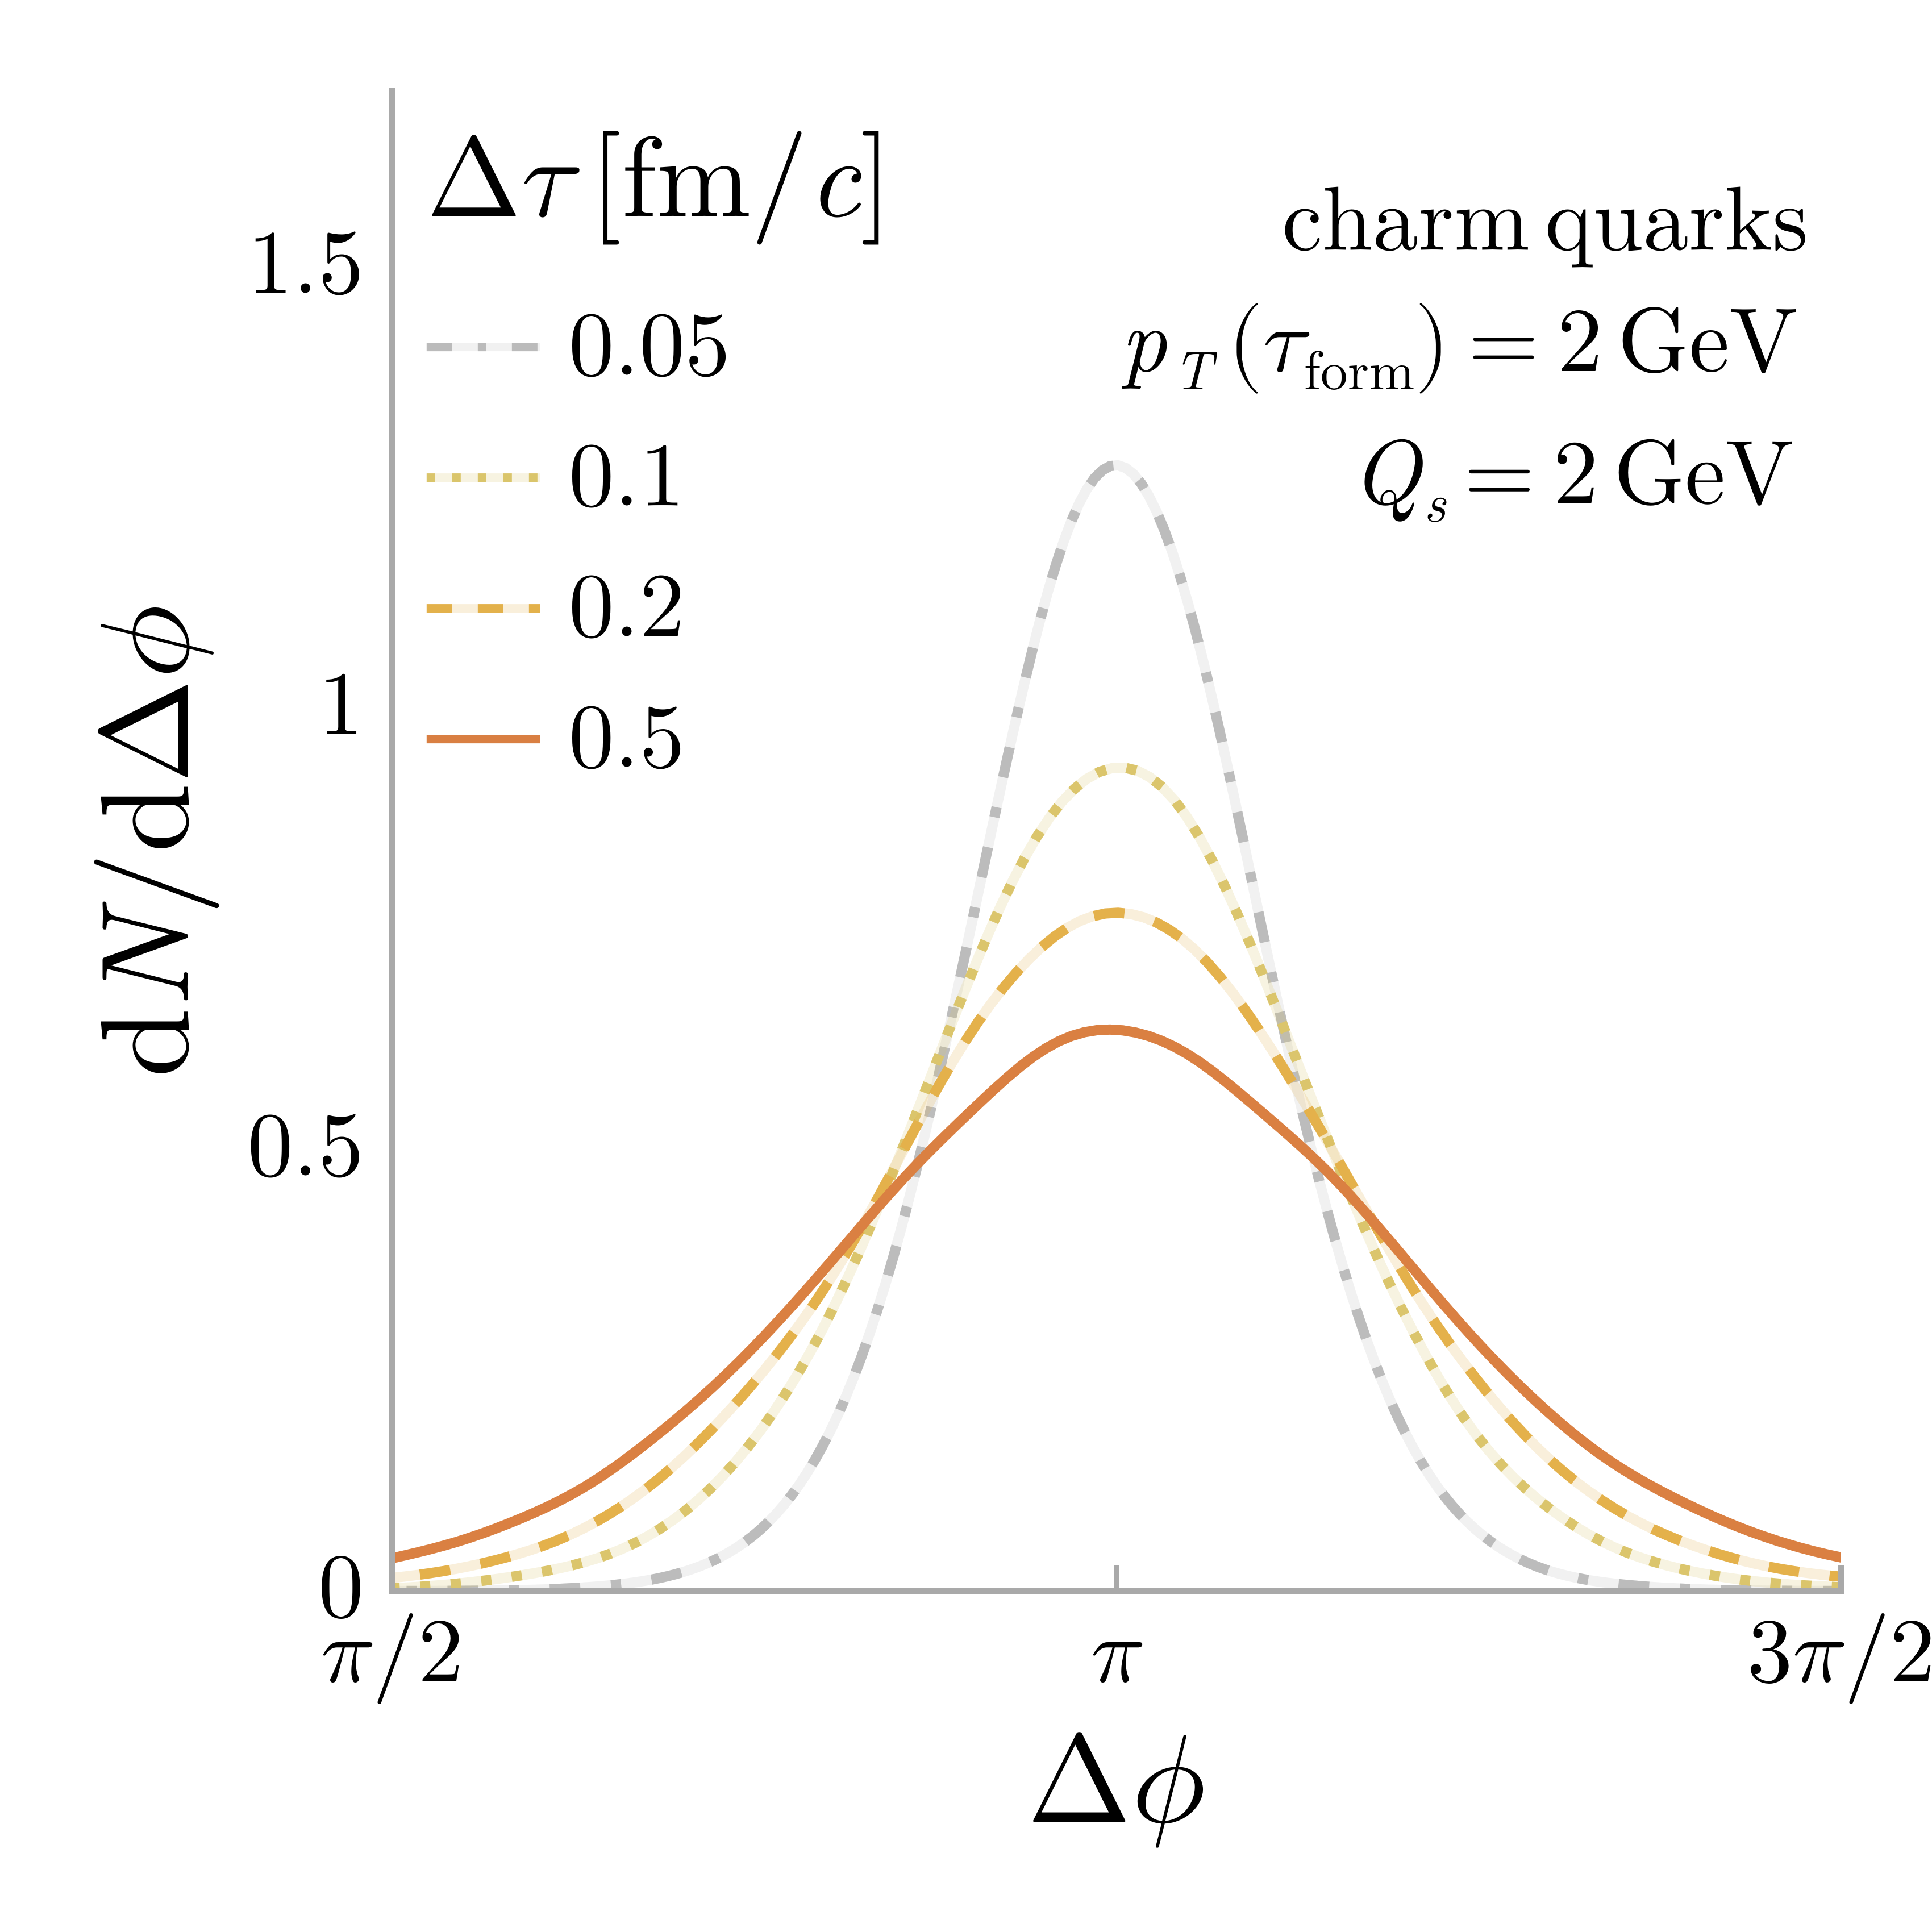
\includegraphics[width=0.7\columnwidth]{images/final_dNdphi_tau_dep_charm_v2.png}
            \end{figure}
            \column{.01\textwidth}
            \column{.49\textwidth}
            \begin{center}
                \begin{custombox2transp}{\normalsize \transparent{0.1}MC@sHQ+EPOS model}{Orange}
                    \small
                    \begin{varwidth}{1.06\textwidth}
                    \begin{itemize}\itemsep0em 
                        \itemsep0em
                        \footnotesize
                        \setbeamertemplate{itemize item}{\raisebox{0.2em}{\scalebox{0.7}{${\color{Orange}\blacktriangleright}$}}} 
                        \item \transparent{0.1}Decorrelation due to {\bfseries\color{Orange}transport in medium}
                        \item \transparent{0.1}Collisional + radiative energy loss effects
                        \item \transparent{0.1}Small $p_T$ pairs {\bfseries\color{Orange}decorrelate throughout evolution}
                    \end{itemize}
                    \end{varwidth}
                \end{custombox2transp}
            \end{center}
            \vspace{-10pt}
            % \vspace{-7pt}
            \begin{figure}
                \centering
                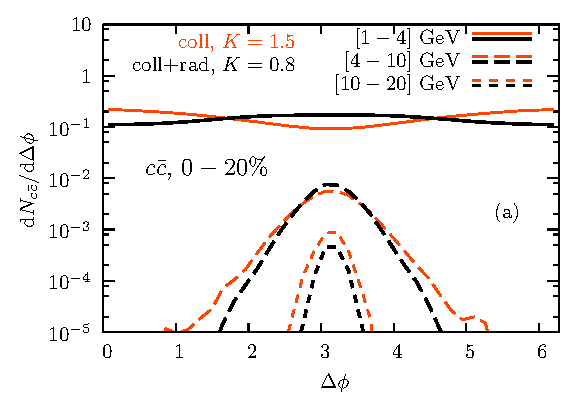
\includegraphics[width=0.83\columnwidth]{images/deltaphi_cccor_centrala.eps}
            \end{figure}
            \column{.02\textwidth}
        \end{columns}    
    \end{center}}

    \begin{center}
        \vspace{-10pt}
        \begin{tikzpicture}[remember picture,overlay]
            \node[align=center] at (0,4) {
                    \begin{custombox2}{\large This study}{palteal}
                        \small
                        \begin{varwidth}{0.58\textwidth}
                        \begin{itemize}\itemsep0em 
                            \itemsep0em
                            % \footnotesize
                            \setbeamertemplate{itemize item}{\raisebox{0.2em}{\scalebox{0.7}{${\color{palteal}\blacktriangleright}$}}} 
                            \item Strong glasma fields quickly deccoralate $Q\overline{Q}$ pairs
                            \item {\bfseries\color{palteal}Model predictions} for $D\overline{D}$ angular correlations will\\
                                benefit from {\bfseries\color{palteal}including the glasma stage}
                        \end{itemize}
                        \end{varwidth}
                    \end{custombox2}
            };
        \end{tikzpicture} 
    \end{center}
    % \vspace{-15pt}
    % \blfootnote{\scriptsize Nahrgang, Aichelin, Gossiaux, Werner \href{https://arxiv.org/abs/1305.3823}{{\color{Orange}\texttt{[1305.3823]$^\text{\tiny\faExternalLink}$}}}}
\end{frame}

%%%%%%%%%%%%%%%%%%%%%%%%%%%%%%%%%%%%%%%%
%%%%%%%%%%%%%%% SECTION %%%%%%%%%%%%%%%%
%%%%%%%%%%%%%%%%%%%%%%%%%%%%%%%%%%%%%%%%

\section{Summary}

%%%%%%%%%%%%%%%%%%%%%%%%%%%%%%%%%%%%%%%%%%%%
%%%%%%%%%%%%%%%%%% SLIDE  %%%%%%%%%%%%%%%%%%
%%%%%%%%%%%%%%%%%%%%%%%%%%%%%%%%%%%%%%%%%%%%

\begin{frame}
    \frametitle{Summary}
    \begin{center}
        \begin{custombox2}{Framework}{palteal}
            \small
            \begin{varwidth}{0.51\textwidth}
            \begin{itemize}\itemsep0em 
                \itemsep0em
                % \footnotesize
                \setbeamertemplate{itemize item}{\raisebox{0.2em}{\scalebox{0.7}{${\color{palteal}\blacktriangleright}$}}} 
                \item Classical transport of heavy quarks in glasma
                % \item \textbf{Anisotropic} momentum broadening
                \item {\color{palteal}\textbf{Large}} transport coefficient {\color{palteal}$\boldsymbol{\kappa}$}
            \end{itemize}
            \end{varwidth}
        \end{custombox2}

        % \vspace{2pt}

        \begin{custombox2}{Main results}{palgold}
            \small
            \begin{varwidth}{0.68\textwidth}
            \begin{itemize}\itemsep0em 
                \itemsep0em
                % \footnotesize
                \setbeamertemplate{itemize item}{\raisebox{0.2em}{\scalebox{0.7}{${\color{palgold}\blacktriangleright}$}}} 
                \item Impact of glasma on $R_{AA}$ weaker than \textbf{\color{palgold}nPDF} effect
                \item Large \textbf{\color{palgold}azimuthal decorrelation} of $Q\overline{Q}$ pairs in glasma \\
                Relevant in model predictions for \textbf{\color{palgold}$\boldsymbol{D\overline{D}}$ measurements} in $AA$
            \end{itemize}
            \end{varwidth}
        \end{custombox2}

        % \vspace{2pt}

        \begin{custombox2}{Improvements}{palviolet}
            \small
            \begin{varwidth}{0.55\textwidth}
            \begin{itemize}\itemsep0em 
                \itemsep0em
                % \footnotesize
                \setbeamertemplate{itemize item}{\raisebox{0.2em}{\scalebox{0.7}{${\color{palviolet}\blacktriangleright}$}}} 
                \item \textbf{\color{palviolet}Energy loss} mechanism in glasma
                \item Couple glasma to effective kinetic theory (\textbf{\color{palviolet}EKT})
            \end{itemize}
            \end{varwidth}
        \end{custombox2}
    \end{center}
\end{frame}

\begin{frame}[plain,noframenumbering]{}
    \vspace{20pt}
    \huge\centering Thank you!
\end{frame}

\begin{frame}[plain,noframenumbering]{}
    \huge\centering Back-up
\end{frame}

\appendix

%%%%%%%%%%%%%%%%%%%%%%%%%%%%%%%%%%%%%%%%%
%%%%%%%%%%%%%%%%% SLIDE %%%%%%%%%%%%%%%%%
%%%%%%%%%%%%%%%%%%%%%%%%%%%%%%%%%%%%%%%%%

\begin{frame}
    \frametitle{Heavy-ion collisions}
    \framesubtitle{Stages at weak coupling}

    \begin{center}
        \begin{tikzpicture}
            \node[anchor=south west,inner sep=0] at (0,0) {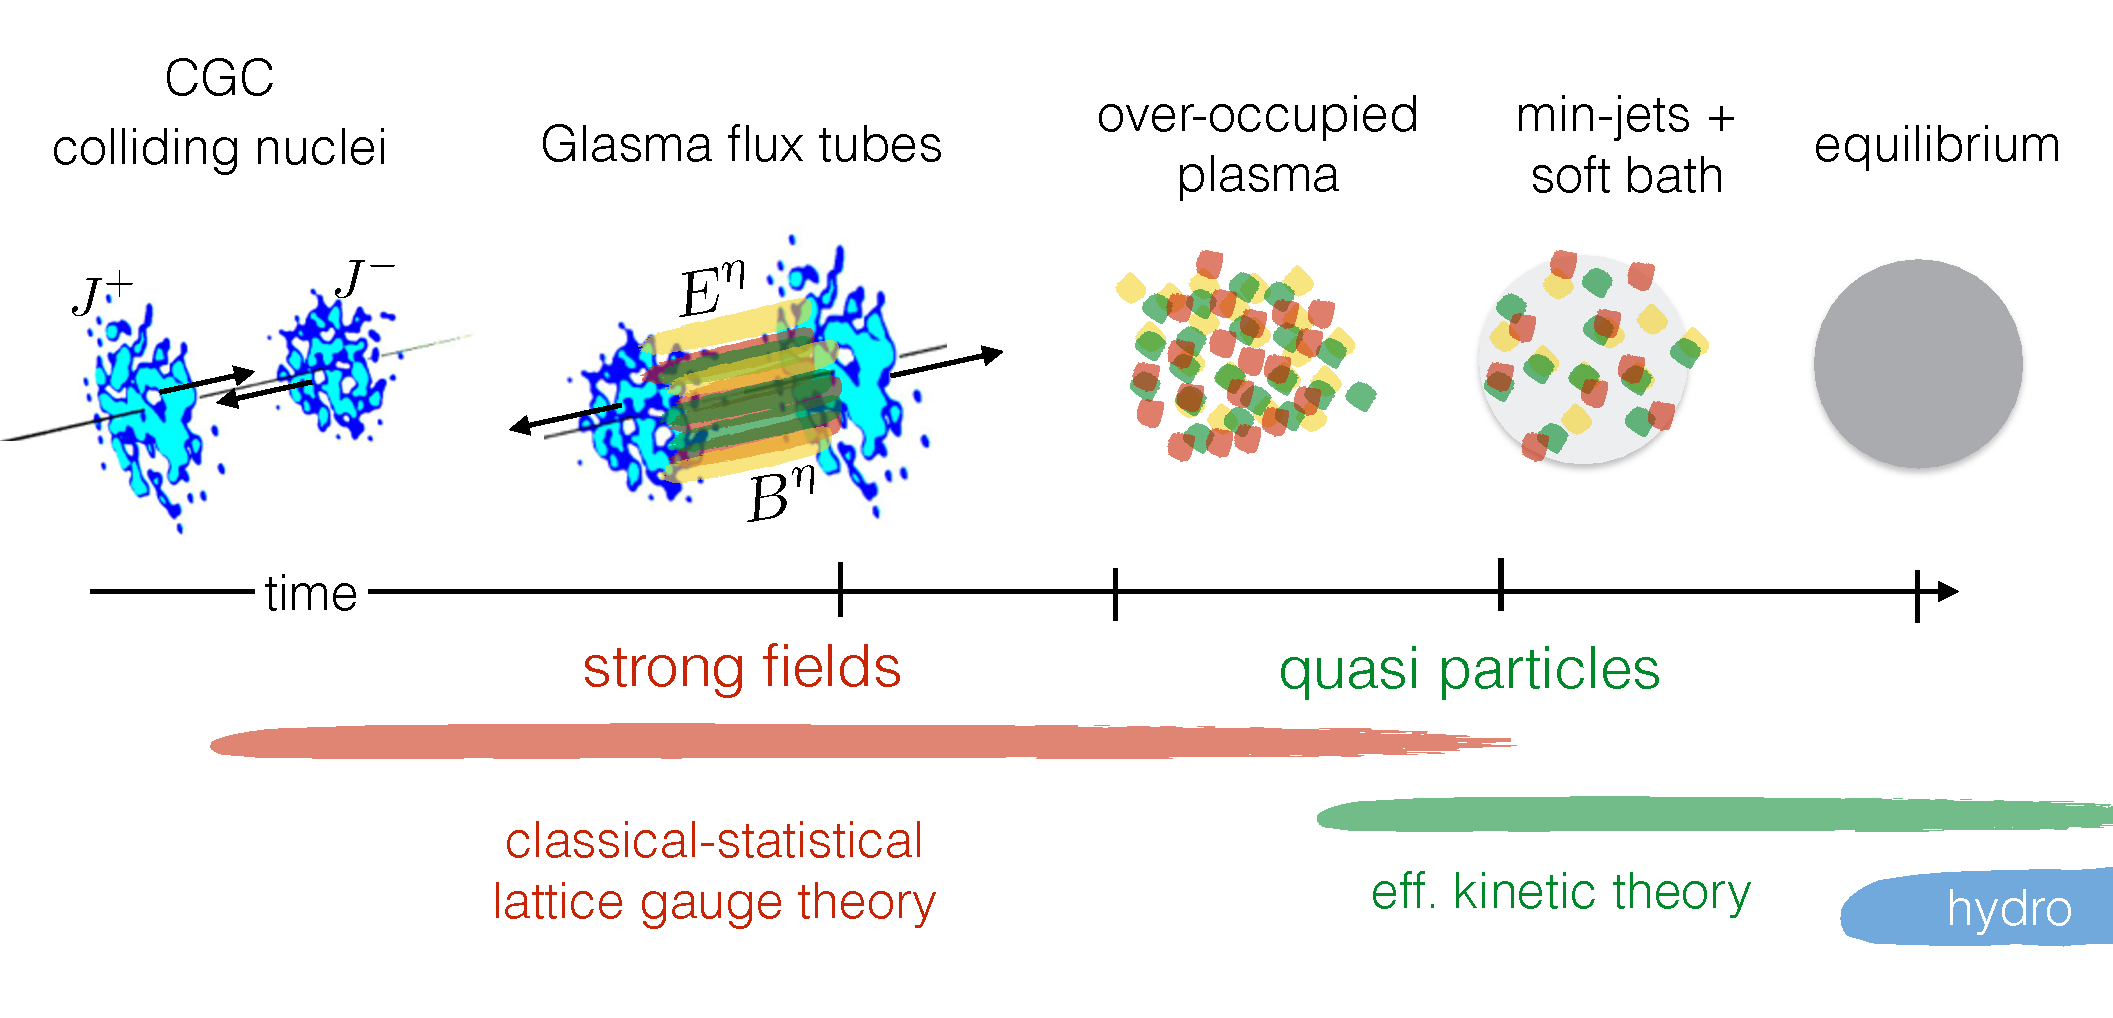
\includegraphics[width=0.8\textwidth]{images/SchlichtingIS2016-pages-cropped.pdf}};
        \end{tikzpicture}
    \end{center}
        
    \blfootnote{\scriptsize Schlichting - \textit{Equilibration at weak coupling} \href{https://indico.cern.ch/event/469857/contributions/1978347/attachments/1277798/1896654/SchlichtingIS2016.pdf}{{\color{palgold}\texttt{[Initial Stages 16]$^\text{\tiny\faExternalLink}$}}}}
\end{frame}


%%%%%%%%%%%%%%%%%%%%%%%%%%%%%%%%%%%%%%%%%
%%%%%%%%%%%%%%%%% SLIDE %%%%%%%%%%%%%%%%%
%%%%%%%%%%%%%%%%%%%%%%%%%%%%%%%%%%%%%%%%%

\setbeamertemplate{itemize item}{\raisebox{0.2em}{\scalebox{0.7}{${\color{palgold}\blacktriangleright}$}}} 

\begin{frame}[noframenumbering]
    \frametitle{Heavy-ion collisions}
    \framesubtitle{The very early stage}
    
    \begin{center}
        \begin{tikzpicture}[]
            \node[anchor=south west,inner sep=0] at (0,0) {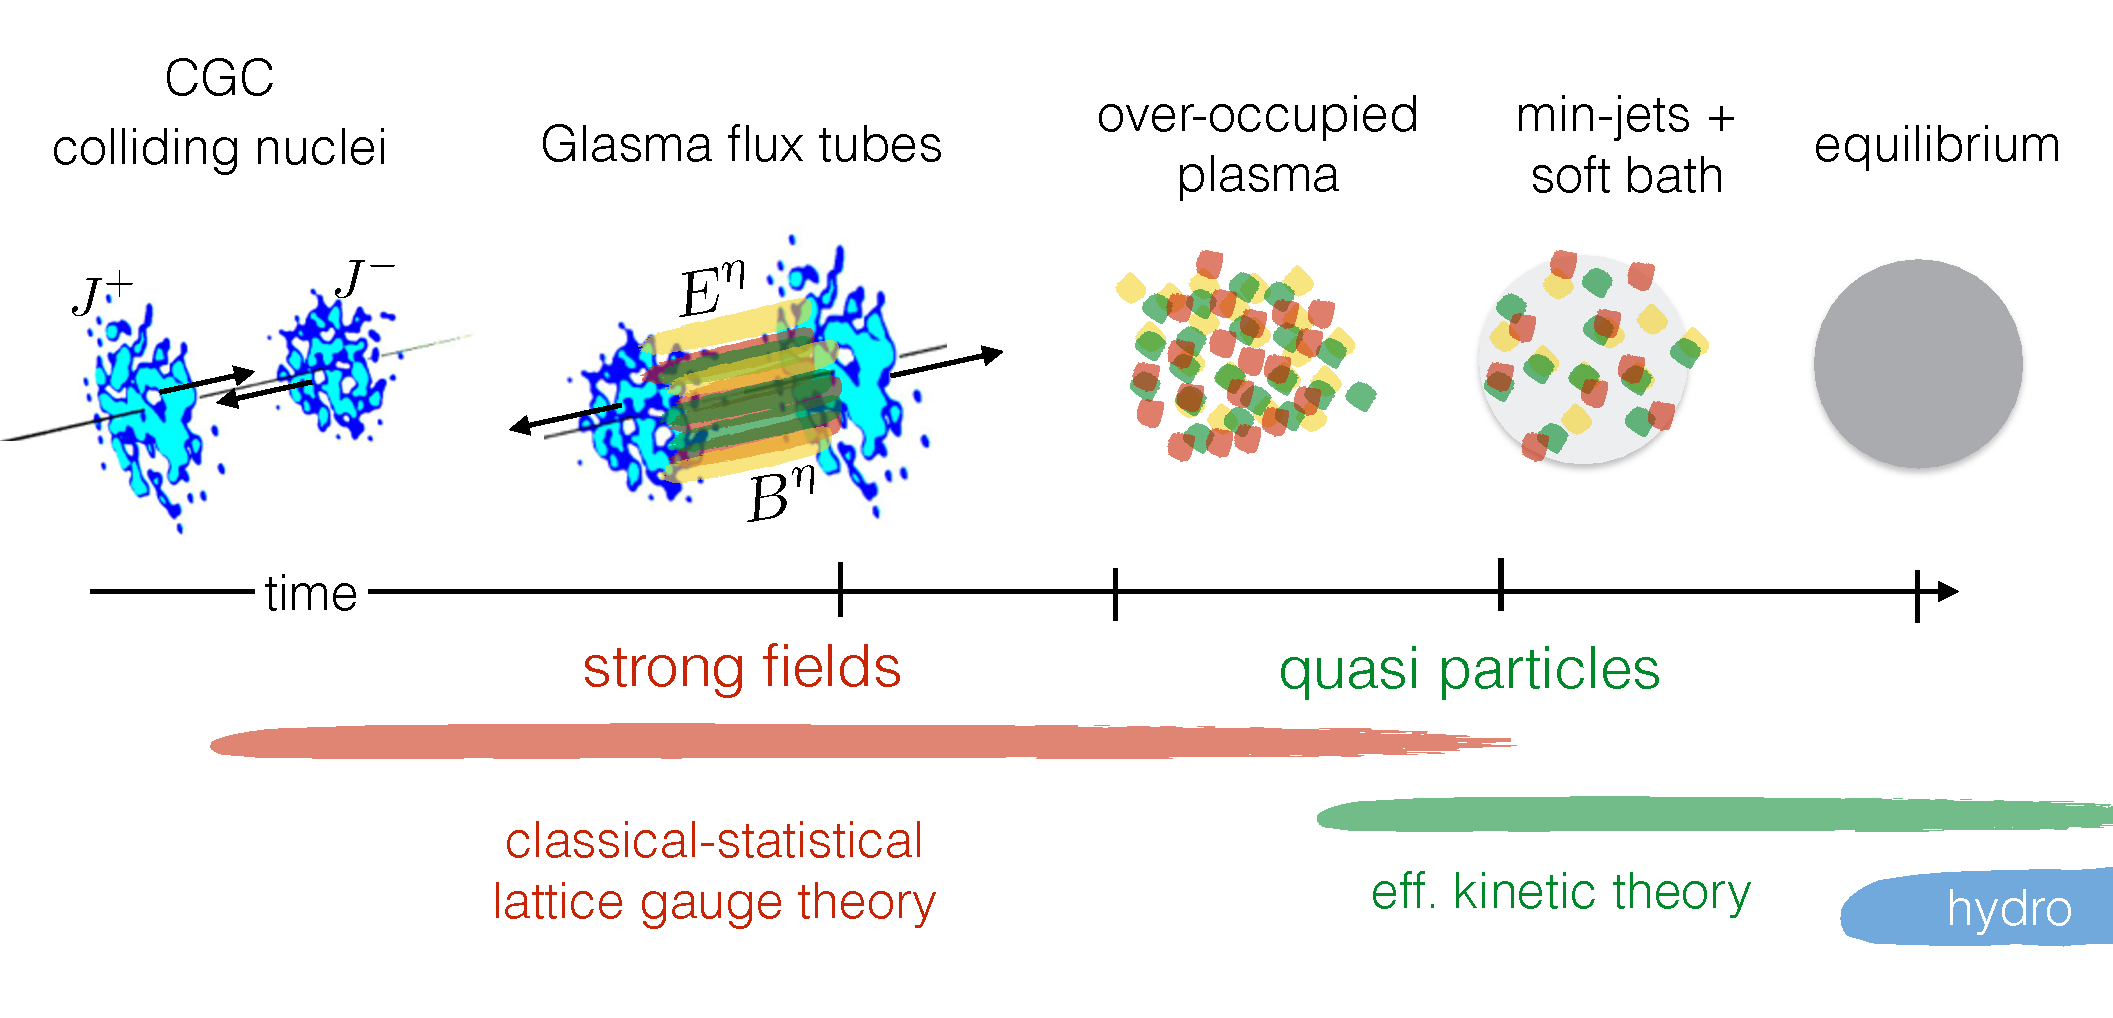
\includegraphics[width=0.8\textwidth]{images/SchlichtingIS2016-pages-cropped.pdf}};
            \draw<1>[white, fill=white, fill opacity=0.9] (6.3,0) rectangle (\textheight+4.6cm,5.5) node[pos=0.5, anchor=center, xshift=0.03\linewidth,text width=6.2cm,align=center] {{\Large\color{palgold}\bfseries Glasma initial stage}\\[10pt]\begin{itemize}\itemsep0em 
                % \footnotesize
                % \item {\color{normal}Framework}: {\bfseries color glass condensate}
                % \item {\color{normal}Regime}: {\bfseries weakly coupled} $\alpha_s\ll 1$
                % \item {\color{normal}Degree of freedom}: {\bfseries gluon fields} $\rightarrow$ occupation $\sim 1/\alpha_s\gg 1$ $\Rightarrow$ {\bfseries classical}
                % \item {\color{normal}Technique}: real-time classical {\bfseries lattice gauge theory}
                % \item {\color{normal}Property}: {\bfseries out-of-equilibrium}
                \item {\bfseries Color glass condensate}
                \item Weakly coupled $\alpha_s\ll 1$
                \item {\bfseries Gluon fields} with occupation number $\sim 1/\alpha_s\gg 1$ $\Rightarrow$ {\bfseries classical}
                \item Real-time {\bfseries lattice gauge theory}
                \item {\bfseries Out-of-equilibrium} medium
                % \item Non-perturbative dynamics
            \end{itemize}
            };
            \draw<1>[palgold,thick,fill=palgold,fill opacity=0.1,rounded corners=3pt] (-0.1,0.3) rectangle (\textheight-1.45cm,5.75);
        \end{tikzpicture}
    \end{center}
        
    \blfootnote{\scriptsize Lappi \href{https://arxiv.org/abs/hep-ph/0606207}{{\color{palgold}\texttt{[hep-ph/0606207]}$^\text{\tiny\faExternalLink}$}}, Gelis \href{https://arxiv.org/abs/1211.3327}{{\color{palgold}\texttt{[1211.3327]}$^\text{\tiny\faExternalLink}$}}}
\end{frame}

%%%%%%%%%%%%%%%%%%%%%%%%%%%%%%%%%%%%%%%%%
%%%%%%%%%%%%%%%%% SLIDE %%%%%%%%%%%%%%%%%
%%%%%%%%%%%%%%%%%%%%%%%%%%%%%%%%%%%%%%%%%

\setbeamertemplate{itemize item}{\raisebox{0.2em}{\scalebox{0.7}{${\color{normal}\blacktriangleright}$}}} 

\begin{frame}
    \frametitle{Color glass condensate}
    \framesubtitle{Effective field theory of QCD at high energies}
    \vspace{-10pt}
    \begin{columns}[onlytextwidth,t]
       \column{.033\textwidth}
       \column{.45\textwidth}

            \begin{itemize}\itemsep0em 
                \footnotesize\color{lightgray}
                \setbeamertemplate{itemize item}{\raisebox{0.2em}{\scalebox{0.6}{${\color{lightgray}\blacktriangleright}$}}}
                \item High-energy nucleus $\rightarrow$ mostly {\color{palviolet}soft gluons}
            \end{itemize}

            \vspace{5pt}
            \hspace{10pt}
            \begin{tikzpicture}[]
                \node[anchor=south west,inner sep=0] at (0,0) {\includegraphics[width=0.7\textwidth]{images/CFNS_talk_Salazar-3_crop_edit_final_v2.png}};
                \draw<1>[palviolet,line width=1pt,fill=palviolet,fill opacity=0.1,rounded corners=3pt] (2.2, 0) rectangle (4.8, 4.9);
            \end{tikzpicture}
        \column{.033\textwidth}
        \column{.45\textwidth}

            \vspace{-5pt}
           
            \begin{custombox2}{Color glass condensate}{lightgray}
                \small
                \begin{varwidth}{0.9\textwidth}
                \begin{itemize}\itemsep0em 
                    \setbeamertemplate{itemize item}{\raisebox{0.2em}{\scalebox{0.7}{${\color{palviolet}\blacktriangleright}$}}} 
                    \item Soft partons $\rightarrow$ {\color{palviolet}\bfseries gauge fields $\boldsymbol{A^\mu}$}
                    \setbeamertemplate{itemize item}{\raisebox{0.2em}{\scalebox{0.7}{${\color{palteal}\blacktriangleright}$}}} 
                    \item Hard partons $\rightarrow$ {\color{palteal}\bfseries color current $\boldsymbol{J^\mu}$}
                \end{itemize}
                \end{varwidth}
            \end{custombox2}

            \begin{itemize}\itemsep0em 
                \footnotesize\color{lightgray}
                \setbeamertemplate{itemize item}{\raisebox{0.2em}{\scalebox{0.6}{${\color{lightgray}\blacktriangleright}$}}}
                \item Classical {\color{palviolet}gluon fields} $\rightarrow$ produced\\ by color {\color{pallightblue}nucleus current}
            \end{itemize}
            \begin{itemize}\itemsep0em 
                \item Classical Yang-Mills equations
            \end{itemize}
            \vspace{25pt}
            \renewcommand{\eqnhighlightheight}{\vphantom{\mathcal{D}_\mu}\mathstrut}\begin{equation*}
                \hspace{0pt}\eqnmark[normal]{dmu}{\mathscr{D}_\mu}\hspace{-3pt}\eqnmark[normal]{fmunu}{F^{\mu\nu}}\hspace{-3pt}={\color{palteal}\boldsymbol{J^\nu}}{\color{lightgray}\rightarrow\text{model input }\,{\color{palteal}J^\nu}} 
                \end{equation*}
                \annotate[yshift=-0.7em]{below, right}{dmu}{\scriptsize $\partial_\mu-\mathrm{i}g{\color{palviolet}\boldsymbol{A_\mu}}$}
                \annotate[yshift=1.2em]{above}{fmunu}{\scriptsize $\partial_\mu{\color{palviolet}\boldsymbol{A_\nu}}-\partial_\nu{\color{palviolet}\boldsymbol{A_\mu}}-\mathrm{i}g[{\color{palviolet}\boldsymbol{A_\mu}},{\color{palviolet}\boldsymbol{A_\nu}}]$}
              
        \column{.033\textwidth}
    \end{columns}
    \blfootnote{\scriptsize Gelis, Iancu, Jalilian-Marian, Venugopalan \href{https://arxiv.org/abs/1002.0333}{{\color{palgold}\texttt{[1002.0333]}$^\text{\tiny\faExternalLink}$}}}
\end{frame}

%%%%%%%%%%%%%%%%%%%%%%%%%%%%%%%%%%%%%%%%%
%%%%%%%%%%%%%%%%% SLIDE %%%%%%%%%%%%%%%%%
%%%%%%%%%%%%%%%%%%%%%%%%%%%%%%%%%%%%%%%%%

\begin{frame}
    \frametitle{Color glass condensate}
    \framesubtitle{MV model for large nuclei}
    \vspace{-10pt}
    \begin{columns}[onlytextwidth,t]
        \column{.033\textwidth}
        \column{.4\textwidth}

        \begin{itemize}\itemsep0em 
            \footnotesize\color{lightgray}
            \setbeamertemplate{itemize item}{\raisebox{0.2em}{\scalebox{0.6}{${\color{lightgray}\blacktriangleright}$}}}
            \item Color charge distribution in a nucleus \\ at high energy $\rightarrow$ thin {\color{palviolet}color sheet}
        \end{itemize}

        \begin{figure}
            \centering
            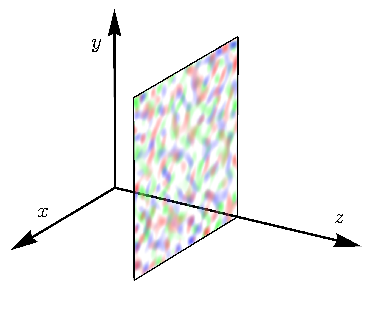
\includegraphics[width=0.9\textwidth]{images/sheets1.pdf}
        \end{figure}
       \column{.033\textwidth}
       \column{.5\textwidth}
       \vspace{-5pt}
        \begin{custombox2}{McLerran Venugopalan model}{lightgray}
            \small
            \begin{varwidth}{0.94\textwidth}
            \begin{itemize}\itemsep0em 
                \setbeamertemplate{itemize item}{\raisebox{0.2em}{\scalebox{0.7}{${\color{palgold}\blacktriangleright}$}}} 
                \item {\color{palgold}\bfseries Color charge} $\color{palgold}\boldsymbol{\rho}$ $\rightarrow$ Gaussian probability
            \end{itemize}
            \end{varwidth}
        \end{custombox2}

        \begin{itemize}\itemsep0em 
            \footnotesize\color{lightgray}
            \setbeamertemplate{itemize item}{\raisebox{0.2em}{\scalebox{0.6}{${\color{lightgray}\blacktriangleright}$}}}
            \item {\color{palteal}Color current} of nucleus $\rightarrow$ generated\\ by {\color{palgold} color charge} density
        \end{itemize}
        \begin{itemize}\itemsep0em 
            \setbeamertemplate{itemize item}{\raisebox{0.2em}{\scalebox{0.7}{${\color{palgold}\blacktriangleright}$}}}
            \item {\bfseries\color{palgold} MV model} for color charges ${\color{palgold}\boldsymbol{\rho}}$
        \end{itemize}
        \vspace{5pt}
        \renewcommand{\eqnhighlightheight}{\vphantom{\mathcal{D}_\mu}\mathstrut}\begin{equation*}
            \big\langle{\color{palgold}\boldsymbol{\rho}}(\vec{x}_\perp){\color{palgold}\boldsymbol{\rho}}(\vec{y}_\perp)\big\rangle\propto\hspace{-3pt}\eqnmark[normal]{g2mu}{{\color{palviolet}\boldsymbol{g^2\mu}}}\hspace{-3pt}^2\delta^{(2)}(\vec{x}_\perp-\vec{y}_\perp)
            \end{equation*}
            \annotate[yshift=-0.7em]{below, right}{g2mu}{\scriptsize ${\color{palviolet}\boldsymbol{g^2\mu}}\propto{\color{palviolet}\boldsymbol{Q_s}}$}
            \vspace{5pt}
            \begin{itemize}\itemsep0em 
                \setbeamertemplate{itemize item}{\raisebox{0.2em}{\scalebox{0.7}{${\color{palviolet}\blacktriangleright}$}}}
                \item {\color{palviolet}\bfseries Saturation momentum $\boldsymbol{Q_s}$} \\{\scriptsize\color{lightgray} $Q_s\approx 2\,\mathrm{GeV}$ at LHC central collisions}
            \end{itemize}    
              
        \column{.033\textwidth}
    \end{columns}
    \blfootnote{\scriptsize McLerran, Venugopalan \href{https://arxiv.org/abs/hep-ph/9309289}{{\color{palgold}\texttt{[hep-ph/9309289]}$^\text{\tiny\faExternalLink}$}}, Müller \href{https://arxiv.org/abs/1904.04267}{{\color{palviolet}\texttt{[1904.04267]}$^\text{\tiny\faExternalLink}$}}}
\end{frame}

%%%%%%%%%%%%%%%%%%%%%%%%%%%%%%%%%%%%%%%%%
%%%%%%%%%%%%%%%%% SLIDE %%%%%%%%%%%%%%%%%
%%%%%%%%%%%%%%%%%%%%%%%%%%%%%%%%%%%%%%%%%

\begin{frame}
    \frametitle{Collision of two nuclei}
    \framesubtitle{How to construct the glasma fields}
    \vspace{-10pt}
    \begin{columns}[onlytextwidth,t]
        \column{.033\textwidth}
        \column{.4\textwidth}

        \begin{itemize}\itemsep0em 
            \item Light-cone diagram of collision\\
            {\scriptsize\color{lightgray} Light-cone coordinates $x^\pm=t\pm z$}
        \end{itemize}
        \begin{tikzpicture}[]
            \node[anchor=south west,inner sep=0] at (0,0) {\includegraphics[width=\textwidth]{images/spacetb.eps}};
            \node[isosceles triangle,
                isosceles triangle apex angle=90,
                draw=palviolet,opacity=0.05,
                fill=palviolet,fill opacity=0.1,
                minimum size =2cm] (T90)at (1.8,2.2){};
            \node[isosceles triangle,
                isosceles triangle apex angle=90,
                draw=palviolet,opacity=0.05,
                fill=palviolet,fill opacity=0.1,
                rotate=180,
                minimum size =2cm] (T90)at (4.25,2.2){};
            \node[isosceles triangle,
                isosceles triangle apex angle=90,
                draw=palgold,opacity=0.05,line width=1pt,
                fill=palgold,fill opacity=0.1,
                rotate=270,
                minimum size =2cm] (T90)at (3.03,3.43){};
        \end{tikzpicture}

       \column{.033\textwidth}
       \column{.5\textwidth}
        \begin{custombox2}{{\normalsize CGC fields} {\tiny (regions 1, 2)}}{palviolet}
            \small
            \begin{varwidth}{0.92\textwidth}
            \begin{itemize}\itemsep0em 
                \setbeamertemplate{itemize item}{\raisebox{0.2em}{\scalebox{0.7}{${\color{palviolet}\blacktriangleright}$}}} 
                \footnotesize
                \item Analytical {\color{red}pure gauge} fields before collision
                \item Transverse ${\color{red}A_i}\propto V^\dagger\partial_i V$,  $V$ Wilson line
            \end{itemize}
            \end{varwidth}
        \end{custombox2}

        \begin{custombox2}{{\normalsize Initial condition} {\tiny (along light-cone)}}{normal}
            \small
            \begin{varwidth}{0.92\textwidth}
            \begin{itemize}\itemsep0em 
                \setbeamertemplate{itemize item}{\raisebox{0.2em}{\scalebox{0.7}{${\color{normal}\blacktriangleright}$}}} 
                \footnotesize
                \item Match CGC fields on the light cone
                \item Impose boost-invariance $A_\mu=\mathrm{indep}({\color{ForestGreen}\eta})$\\
                {\tiny\color{lightgray} Milne coordinates {\color{Blue}$\tau=\sqrt{x^+x^-}$} and {\color{ForestGreen}$\eta=\mathrm{ln}(x^+/x^-)$}}
            \end{itemize}
            \end{varwidth}
        \end{custombox2}

        \begin{custombox2}{{\normalsize Glasma fields} {\tiny (region 3)}}{palgold}
            \small
            \begin{varwidth}{0.92\textwidth}
            \begin{itemize}\itemsep0em 
                \setbeamertemplate{itemize item}{\raisebox{0.2em}{\scalebox{0.7}{${\color{palgold}\blacktriangleright}$}}} 
                \footnotesize
                \item Numerically solve CYM equations
                \item Code \href{https://gitlab.com/openpixi/curraun}{\color{palgold}\texttt{gitlab.com/openpixi/curraun}$^\text{\tiny\faGitlab}$}
            \end{itemize}
            \end{varwidth}
        \end{custombox2}
        \column{.033\textwidth}
    \end{columns}
    \blfootnote{\scriptsize Lappi \href{https://arxiv.org/abs/hep-ph/0602189}{{\color{palgold}\texttt{[hep-ph/0602189]}$^\text{\tiny\faExternalLink}$}}}
\end{frame}

% %%%%%%%%%%%%%%%%%%%%%%%%%%%%%%%%%%%%%%%%%
% %%%%%%%%%%%%%% SUBSECTION %%%%%%%%%%%%%%%
% %%%%%%%%%%%%%%%%%%%%%%%%%%%%%%%%%%%%%%%%%

% \subsection{Transport coefficients}

% %%%%%%%%%%%%%%%%%%%%%%%%%%%%%%%%%%%%%%%%%
% %%%%%%%%%%%%%%%%% SLIDE %%%%%%%%%%%%%%%%%
% %%%%%%%%%%%%%%%%%%%%%%%%%%%%%%%%%%%%%%%%%

\begin{frame}
    \frametitle{Transport coefficient $\kappa$}
    % \framesubtitle{Momentum broadening in glasma}
    \vspace{-10pt}
    \begin{columns}[onlytextwidth,t]
        \column{.033\textwidth}
        \column{.5\textwidth}

        \begin{figure}
            \centering
            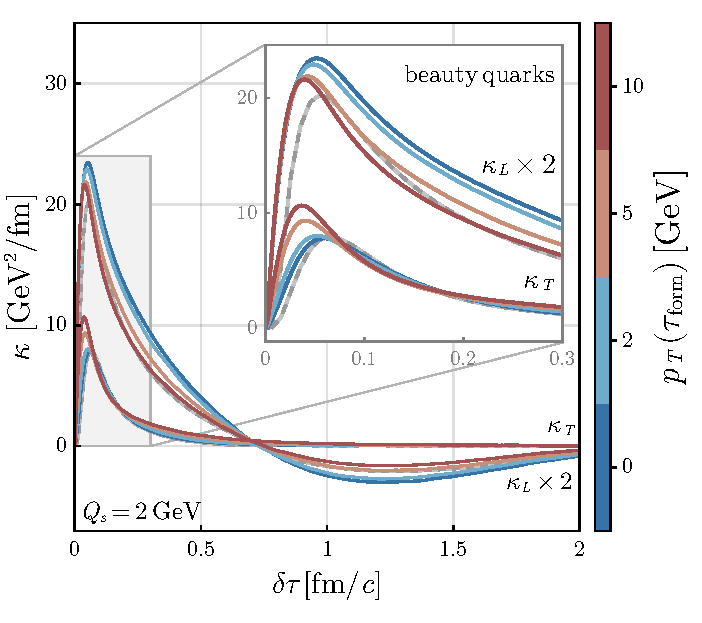
\includegraphics[width=0.9\textwidth]{images/hp23_mom_broad_kappa_anis_wong_vs_kappa-cropped.pdf}
        \end{figure}
       \column{.033\textwidth}
       \column{.4\textwidth}
        \begin{custombox2}{Classical transport}{lightgray}
            \small
            \begin{varwidth}{0.95\textwidth}
            \begin{itemize}\itemsep0em 
                \setbeamertemplate{itemize item}{\raisebox{0.2em}{\scalebox{0.7}{${\color{MidnightBlue}\blacktriangleright}$}}} 
                \item {\color{MidnightBlue}\bfseries Momentum broadening}\\ ${\color{MidnightBlue}\boldsymbol{\delta p^2_i}}(\tau)=p^2_i(\tau)-p^2_i(\tau_\mathrm{form})$
                \setbeamertemplate{itemize item}{\raisebox{0.2em}{\scalebox{0.7}{${\color{Maroon}\blacktriangleright}$}}} 
                \item {\color{Maroon}\bfseries Transport coefficient}\\ ${\color{Maroon}\boldsymbol{\kappa_i}}(\tau)=\dfrac{\mathrm{d}}{\mathrm{d}\tau}\langle{\color{MidnightBlue}\boldsymbol{\delta p^2_i}}(\tau)\rangle$ 
                \\[5pt]
                {\scriptsize\color{lightgray} Formation time $\tau_\mathrm{form}=1/2m$\\[1pt]
                Relative time $\delta\tau=\tau-\tau_\mathrm{form}$\\[-2pt]
                Longitudinal $i=L$, transverse $i=T$}
            \end{itemize}
            \end{varwidth}
        \end{custombox2}

        \begin{itemize}\itemsep0em 
            \footnotesize
            \setbeamertemplate{itemize item}{\raisebox{0.2em}{\scalebox{0.7}{${\color{lightgray}\blacktriangleright}$}}}
            {\color{lightgray}\item {\bfseries Anisotropic} $\kappa_L\neq\kappa_T$
            \item Rapid increase in $\kappa$ at early times 
            \item Negative $\kappa_L$ at late times}
            \setbeamertemplate{itemize item}{\raisebox{0.2em}{\scalebox{0.7}{${\color{palgold}\blacktriangleright}$}}} 
            \item {\bfseries\color{palgold}Large $\boldsymbol{\kappa}$ peak in glasma}
            \setbeamertemplate{itemize item}{\raisebox{0.2em}{\scalebox{0.7}{${\color{palviolet}\blacktriangleright}$}}}
            \item {\bfseries\color{palviolet}Approximate agreement with $\boldsymbol{\kappa}$ during EKT} {\color{lightgray}but not quantitative yet}
        \end{itemize}    
              
        \column{.033\textwidth}
    \end{columns}
    \vspace{-10pt}
    \blfootnote{\scriptsize Avramescu, Băran, Greco, Ipp, Müller, Ruggieri  \href{https://arxiv.org/abs/2307.07999}{{\color{palgold}\texttt{[2307.07999]}$^\text{\tiny\faExternalLink}$}}\\
    \hspace{16.5pt}Boguslavski, Kurkela, Lappi, Lindenbauer, Peuron \href{https://arxiv.org/abs/2303.12520}{{\color{palviolet}\texttt{[2303.12520]}$^\text{\tiny\faExternalLink}$}}
    }
\end{frame}

% %%%%%%%%%%%%%%%%%%%%%%%%%%%%%%%%%%%%%%%%%
% %%%%%%%%%%%%%%%%% SLIDE %%%%%%%%%%%%%%%%%
% %%%%%%%%%%%%%%%%%%%%%%%%%%%%%%%%%%%%%%%%%

\begin{frame}[noframenumbering]
    \frametitle{Transport coefficient $\kappa$}
    % \framesubtitle{Momentum broadening in glasma}
    % \vspace{-10pt}
    \begin{columns}[onlytextwidth,t]
        \column{.033\textwidth}
        \column{.5\textwidth}

        \begin{figure}
            \centering
            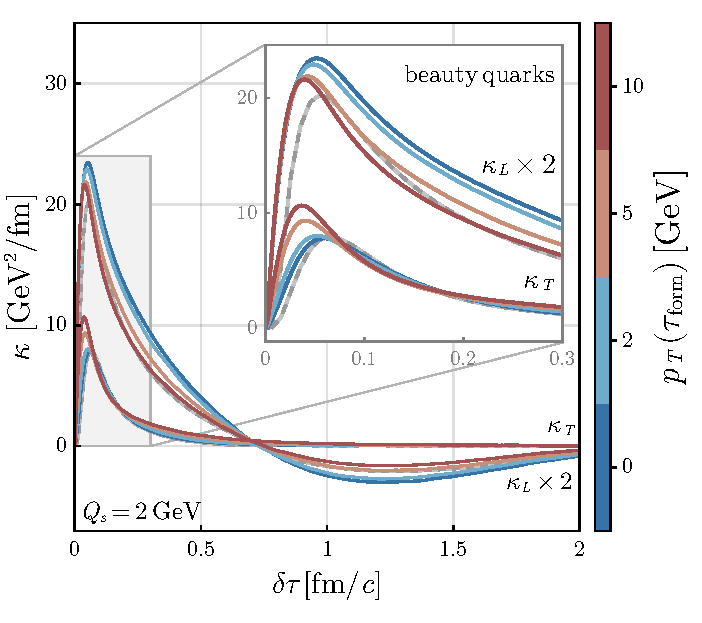
\includegraphics[width=0.9\textwidth]{images/hp23_mom_broad_kappa_anis_wong_vs_kappa-cropped.pdf}
        \end{figure}
       \column{.033\textwidth}
       \column{.4\textwidth}
       \begin{custombox2}{Classical transport}{lightgray}
        \small
        \begin{varwidth}{0.95\textwidth}
        \begin{itemize}\itemsep0em 
            \setbeamertemplate{itemize item}{\raisebox{0.2em}{\scalebox{0.7}{${\color{MidnightBlue}\blacktriangleright}$}}} 
            \item {\color{MidnightBlue}\bfseries Momentum broadening}\\ ${\color{MidnightBlue}\boldsymbol{\delta p^2_i}}(\tau)=p^2_i(\tau)-p^2_i(\tau_\mathrm{form})$
            \setbeamertemplate{itemize item}{\raisebox{0.2em}{\scalebox{0.7}{${\color{Maroon}\blacktriangleright}$}}} 
            \item {\color{Maroon}\bfseries Transport coefficient}\\ ${\color{Maroon}\boldsymbol{\kappa_i}}(\tau)=\dfrac{\mathrm{d}}{\mathrm{d}\tau}\langle{\color{MidnightBlue}\boldsymbol{\delta p^2_i}}(\tau)\rangle$ 
            \\[5pt]
            {\scriptsize\color{lightgray} Formation time $\tau_\mathrm{form}=1/2m$\\[1pt]
            Relative time $\delta\tau=\tau-\tau_\mathrm{form}$\\[-2pt]
            Longitudinal $i=L$, transverse $i=T$}
        \end{itemize}
        \end{varwidth}
    \end{custombox2}

        \begin{custombox2}{Limitation}{palgold}
            \small
            \begin{varwidth}{0.77\textwidth}
            \begin{itemize}\itemsep0em 
                \setbeamertemplate{itemize item}{\raisebox{0.2em}{\scalebox{0.7}{${\color{palgold}\blacktriangleright}$}}} 
                \item Transport coefficients $\neq$ {\color{palgold}\bfseries measurable} quantities
            \end{itemize}
            \end{varwidth}
        \end{custombox2} 
              
        \column{.033\textwidth}
    \end{columns}
    \blfootnote{\scriptsize Avramescu, Băran, Greco, Ipp, Müller, Ruggieri  \href{https://arxiv.org/abs/2307.07999}{{\color{palgold}\texttt{[2307.07999]}$^\text{\tiny\faExternalLink}$}}}
\end{frame}

%%%%%%%%%%%%%%%%%%%%%%%%%%%%%%%%%%%%%%%%%
%%%%%%%%%%%%%%%%% SLIDE %%%%%%%%%%%%%%%%%
%%%%%%%%%%%%%%%%%%%%%%%%%%%%%%%%%%%%%%%%%

\begin{frame}
    \frametitle{Nuclear modification factor}
    \framesubtitle{Extraction of $R_{AA}$ in glasma}
    \vspace{-10pt}
    \begin{columns}[onlytextwidth,t]
        \column{.033\textwidth}
        \column{.43\textwidth}
       \begin{center}
        \begin{custombox2}{$\boldsymbol{R_{AA}}$ in glasma}{lightgray}
            \small
            \begin{varwidth}{1.05\textwidth}
            \begin{itemize}\itemsep0em 
                \itemsep0em
                \setbeamertemplate{itemize item}{\raisebox{0.2em}{\scalebox{0.7}{${\color{lightgray}\blacktriangleright}$}}} 
                \item Ratio of ${\color{raapink}\boldsymbol{AA}}$ to ${\color{raablue}\boldsymbol{pp}}$ normalized spectra
            \end{itemize}
            \end{varwidth}
        \end{custombox2}

        \begin{itemize}\itemsep0em 
            \itemsep0em
            \footnotesize\color{lightgray}
            \setbeamertemplate{itemize item}{\raisebox{0.2em}{\scalebox{0.7}{${\color{lightgray}\blacktriangleright}$}}} 
            \item ${\color{raapink}\boldsymbol{AA}}$ evolved in {\color{raapink}\bfseries glasma}, ${\color{raablue}\boldsymbol{pp}}$ from {\color{raablue}\bfseries FONLL} 
            \item Glasma spectrum initialized with FONLL
        \end{itemize}
        \vspace{5pt}

        \renewcommand{\eqnhighlightheight}{\vphantom{\mathcal{D}_\mu}\mathstrut}
        \begin{equation*}
            \hspace{0pt}
            R_{AA}(\tau)=\dfrac{1}{A^2}\dfrac{{\color{palteal}\sigma}^{\textcolor{normal}{AA}}_{\mathrm{\textcolor{palteal}{tot}}}}{\eqnmark[palteal]{sigma}{{\color{palteal}\sigma}^{\textcolor{normal}{pp}}_{\mathrm{\textcolor{palteal}{tot}}}}}\dfrac{\eqnmark[raapink]{gl}{\mathrm{d}N/\mathrm{d}p_T}(\tau)}{\eqnmark[raablue]{fonll}{\mathrm{d}N^{pp}/\mathrm{d}p_T}}
        \end{equation*}
        \annotate[yshift=-0.5em]{below, left}{sigma}{\tiny normalization}
        \annotate[yshift=1.2em]{above, left}{gl}{\tiny glasma}
        \annotate[yshift=-0.5em]{below, left}{fonll}{\tiny FONLL}

       \end{center}
       \column{.033\textwidth}
       \column{.47\textwidth}
        \begin{center}
            \begin{custombox2}{\small$\boldsymbol{R_{AA}}$ in glasma explained}{palteal}
                \small
                \begin{varwidth}{\textwidth}
                \begin{itemize}\itemsep0em 
                    \itemsep0em
                    \scriptsize
                    \setbeamertemplate{itemize item}{\raisebox{0.2em}{\scalebox{0.7}{${\color{palteal}\blacktriangleright}$}}} 
                    \item Small $p_T$ particles only migrate to larger $p_T$
                    \item Depletion at small $p_T$, enhancement at large $p_T$
                \end{itemize}
                \end{varwidth}
            \end{custombox2}
            \vspace{-15pt}
            \begin{figure}
                \centering
                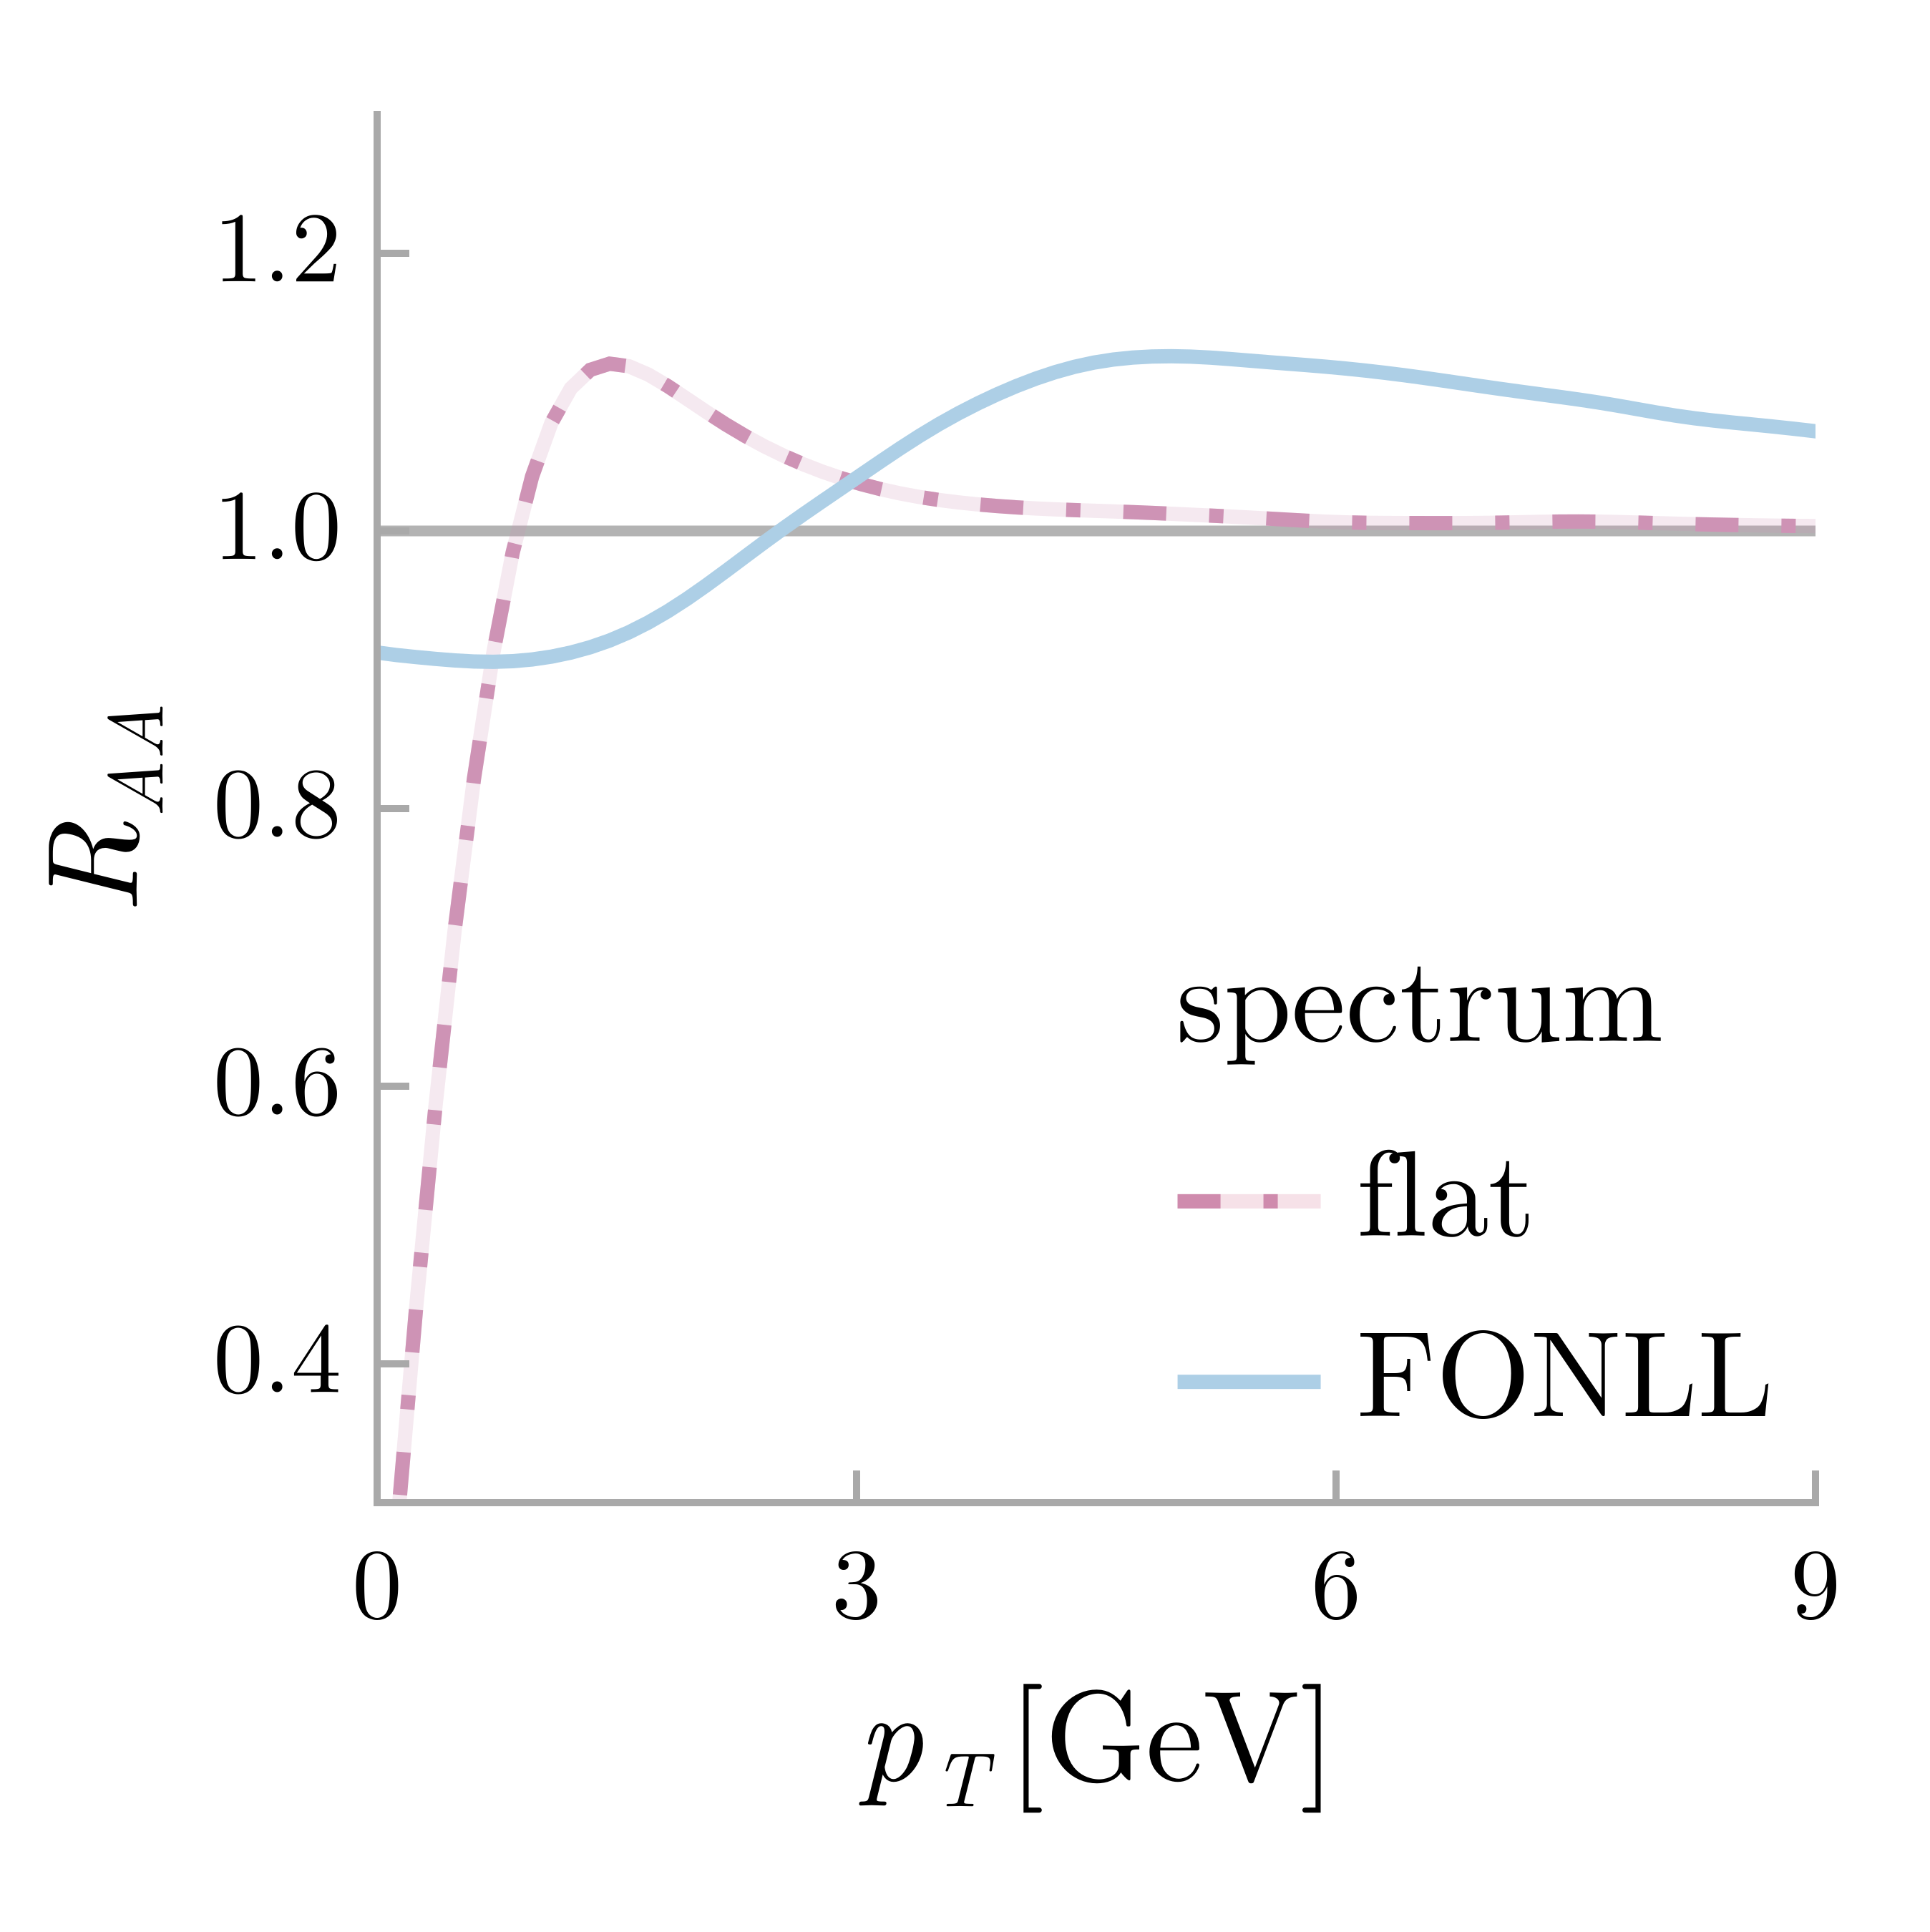
\includegraphics[width=0.7\textwidth]{images/final_sketch_raa_gl_fonll_v4_crop_2.png}
            \end{figure}
        \end{center}
       
        \column{.033\textwidth}
    \end{columns}
\end{frame}


%%%%%%%%%%%%%%%%%%%%%%%%%%%%%%%%%%%%%%%%%
%%%%%%%%%%%%%%%%% SLIDE %%%%%%%%%%%%%%%%%
%%%%%%%%%%%%%%%%%%%%%%%%%%%%%%%%%%%%%%%%%

\begin{frame}
    \frametitle{$R_{AA}$ in glasma}
    % \framesubtitle{Temporal evolution, energy dependence}
    \vspace{-15pt}
    \begin{center}
        \begin{columns}[onlytextwidth,t]
            \column{.02\textwidth}
           \column{.47\textwidth}
           \begin{center}
                \begin{custombox2}{\normalsize Time $\boldsymbol{\tau}$ evolution}{palteal}
                    \small
                    \begin{varwidth}{0.88\textwidth}
                    \begin{itemize}\itemsep0em 
                        \itemsep0em
                        \footnotesize
                        \setbeamertemplate{itemize item}{\raisebox{0.2em}{\scalebox{0.7}{${\color{palteal}\blacktriangleright}$}}} 
                        \item More enhancement in $R_{AA}$ at later $\tau$
                    \end{itemize}
                    \end{varwidth}
                \end{custombox2}
            \end{center}
            \vspace{-10pt}
           \begin{figure}
                \centering
                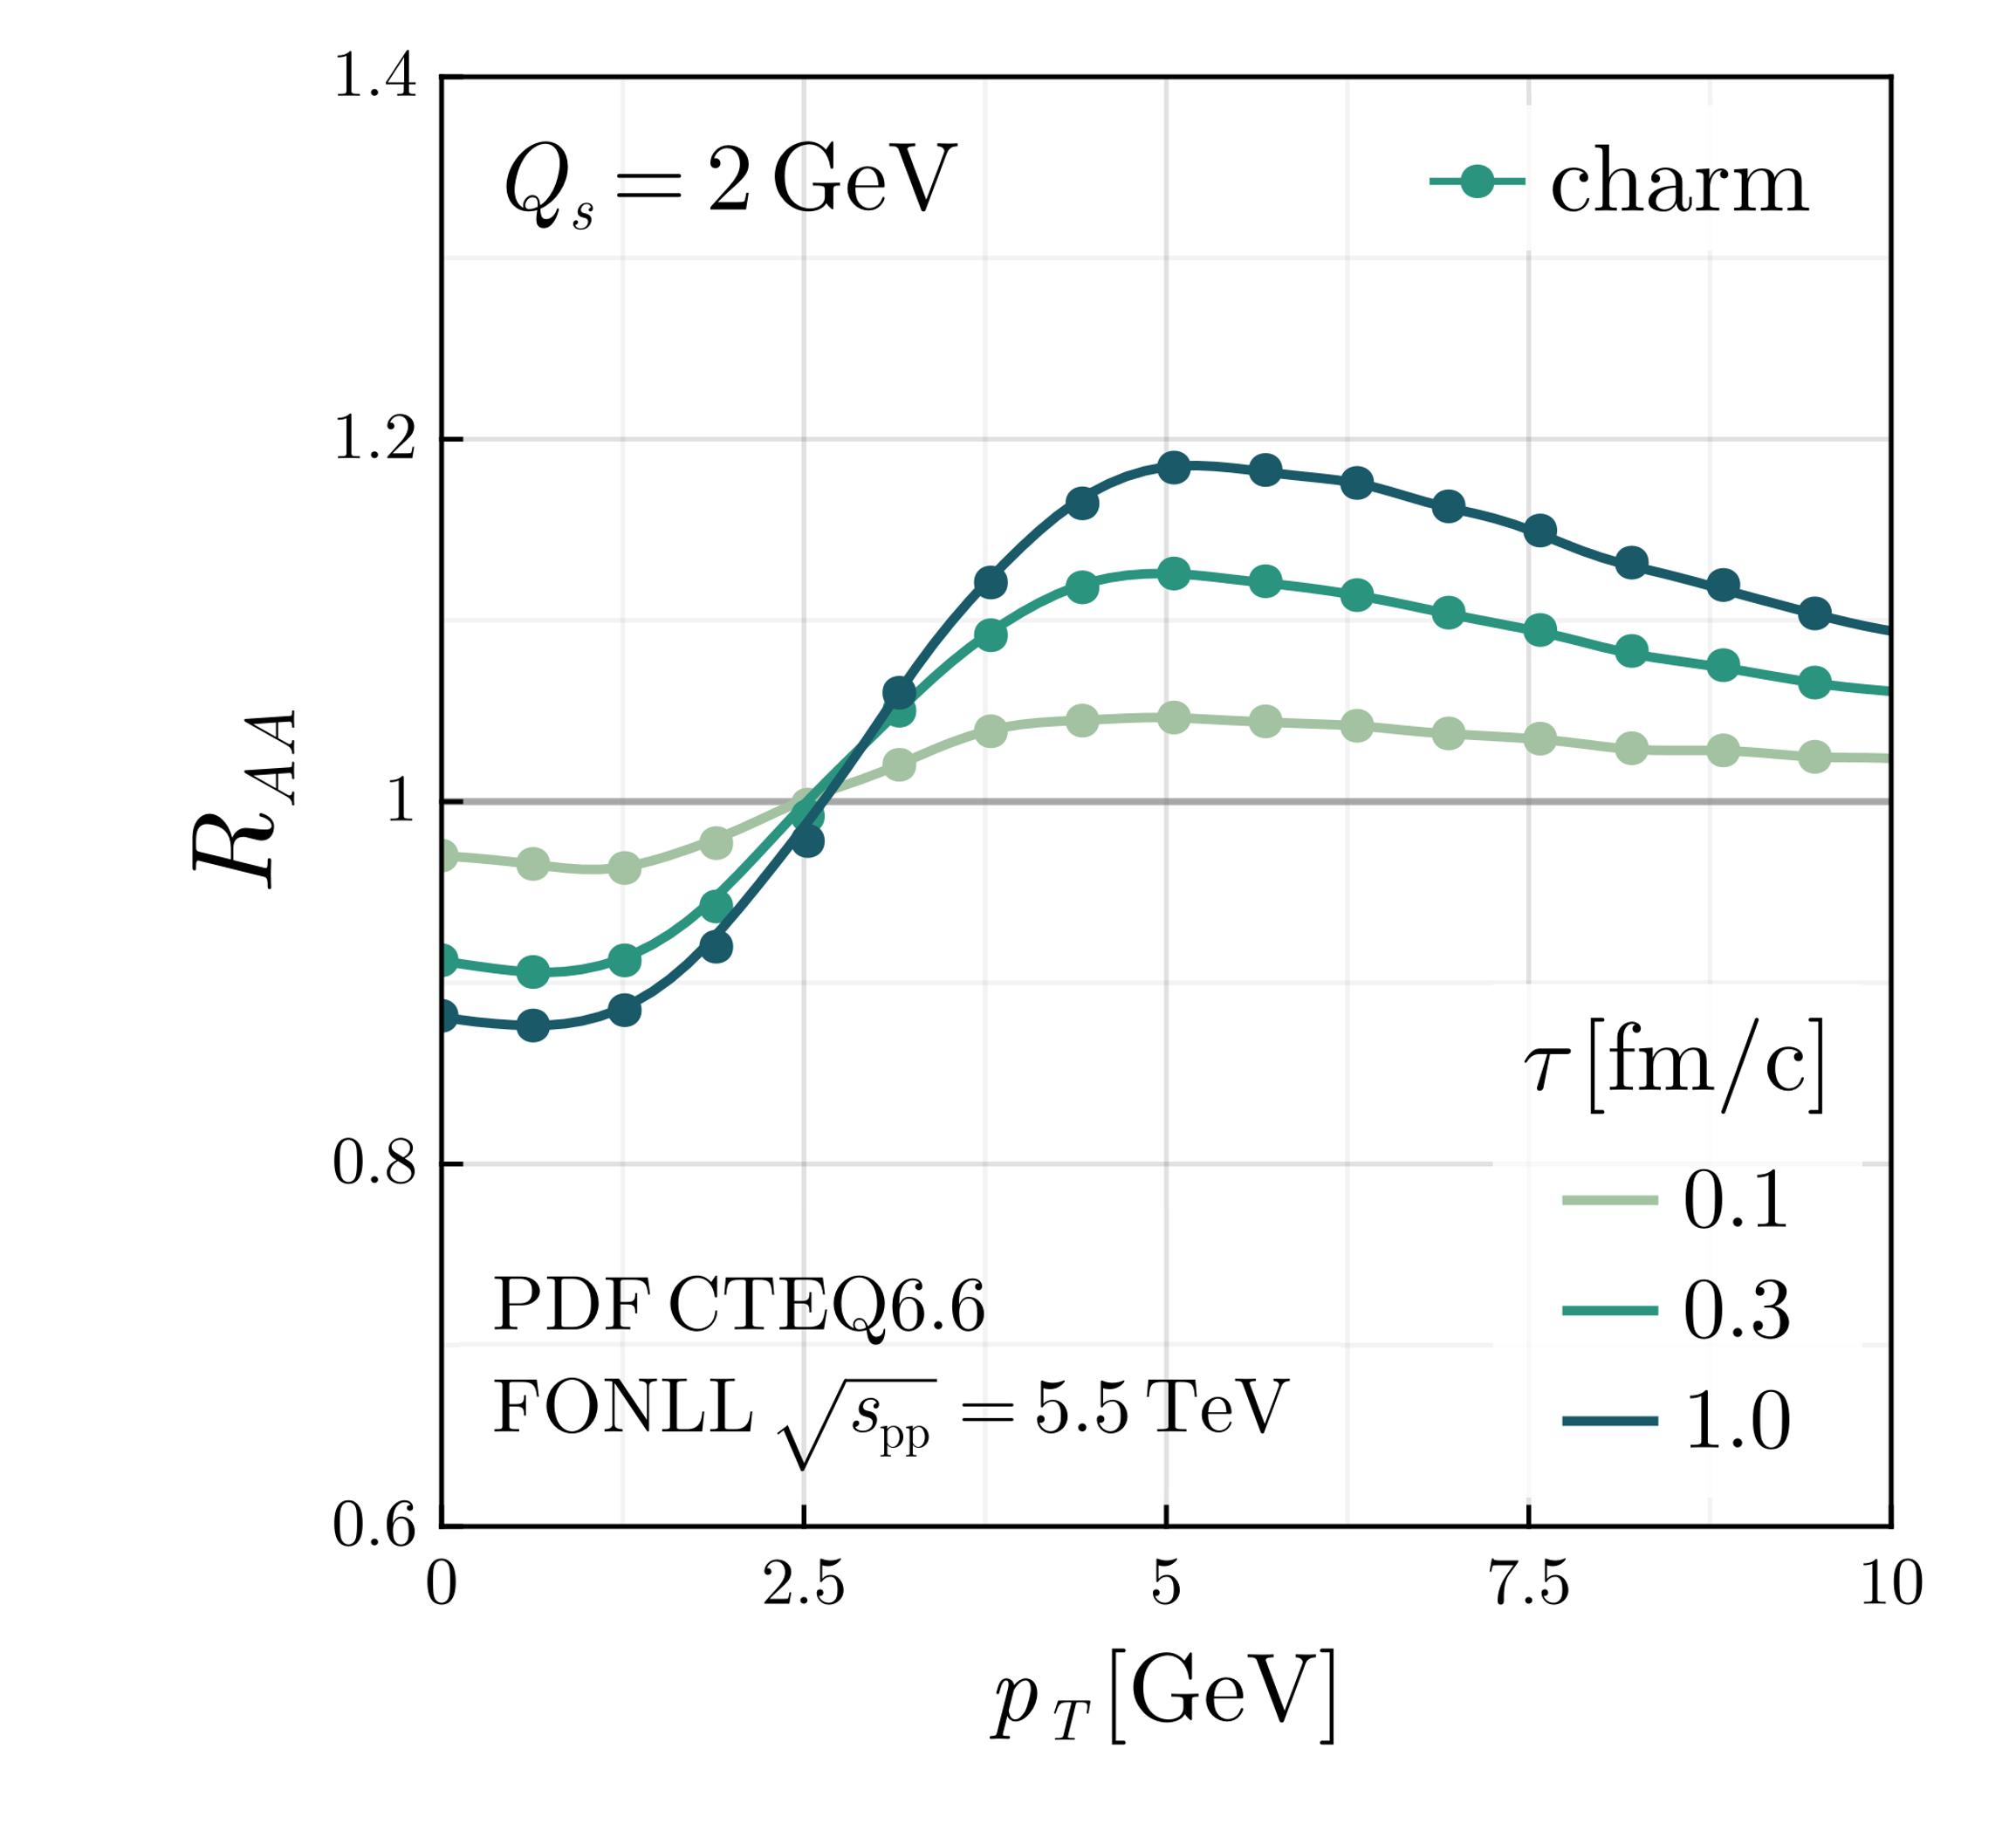
\includegraphics[width=0.9\columnwidth]{images/clean_raa_tau_dep_quarks_charmQs_2.0_fonll_energy_5500_pdf_cteq.png}
            \end{figure}
            \column{.02\textwidth}
            \column{.47\textwidth}
            \begin{center}
                \begin{custombox2}{\normalsize Effect of energy scales}{raapink}
                    \small
                    \begin{varwidth}{0.97\textwidth}
                    \begin{itemize}\itemsep0em 
                        \itemsep0em
                        \footnotesize
                        \setbeamertemplate{itemize item}{\raisebox{0.2em}{\scalebox{0.7}{${\color{raapink}\blacktriangleright}$}}} 
                        \item Weak dependence on $\sqrt{s_\mathrm{pp}}$ and glasma $Q_s$
                    \end{itemize}
                    \end{varwidth}
                \end{custombox2}
            \end{center}
            \vspace{-10pt}
            \vspace{-7pt}
            \begin{figure}
                \centering
                \includegraphics[width=0.83\columnwidth]{images/clean_raa_tau_dep_charm_quark_Qs_fonll_energy_dep_qsenergymap_v3.png}
            \end{figure}
            \column{.02\textwidth}
        \end{columns}    
    \end{center}
\end{frame}


%%%%%%%%%%%%%%%%%%%%%%%%%%%%%%%%%%%%%%%%%
%%%%%%%%%%%%%%%%% SLIDE %%%%%%%%%%%%%%%%%
%%%%%%%%%%%%%%%%%%%%%%%%%%%%%%%%%%%%%%%%%

\begin{frame}
    \frametitle{Azimuthal decorrelation}
    % \framesubtitle{Effect of heavy quark $p_T$ and glasma $Q_s$}
    \vspace{-15pt}
    \begin{center}
        \begin{columns}[onlytextwidth,t]
            \column{.02\textwidth}
           \column{.47\textwidth}
           \begin{center}
                \begin{custombox2}{\normalsize Effect of heavy quark $\boldsymbol{p_T}$}{palteal}
                    \small
                    \begin{varwidth}{0.92\textwidth}
                    \begin{itemize}\itemsep0em 
                        \itemsep0em
                        \footnotesize
                        \setbeamertemplate{itemize item}{\raisebox{0.2em}{\scalebox{0.7}{${\color{palteal}\blacktriangleright}$}}} 
                        \item Small $p_T$ pairs immediately decorrelate  
                    \end{itemize}
                    \end{varwidth}
                \end{custombox2}
            \end{center}
            \vspace{-10pt}
           \begin{figure}
                \centering
                \includegraphics[width=0.95\columnwidth]{images/sigma_dphideta_tau_charm_beauty_pT_dep_final_azimuth.png}
            \end{figure}
            \column{.02\textwidth}
            \column{.47\textwidth}
            \begin{center}
                \begin{custombox2}{\normalsize Effect of glasma $\boldsymbol{Q_s}$}{palblue}
                    \small
                    \begin{varwidth}{0.95\textwidth}
                    \begin{itemize}\itemsep0em 
                        \itemsep0em
                        \footnotesize
                        \setbeamertemplate{itemize item}{\raisebox{0.2em}{\scalebox{0.7}{${\color{palblue}\blacktriangleright}$}}} 
                        \item Large $Q_s$ glasma decorrelates pairs faster
                    \end{itemize}
                    \end{varwidth}
                \end{custombox2}
            \end{center}
            \vspace{-10pt}
            % \vspace{-7pt}
            \begin{figure}
                \centering
                \includegraphics[width=0.95\columnwidth]{images/sigma_dphideta_tau_charm_beauty_Qs_dep_scaled_final_azimuth.png}
            \end{figure}
            \column{.02\textwidth}
        \end{columns}    
    \end{center}
\end{frame}


\end{document}